% this is a comment
%
% This class defines the type of text; instead of 'article' one could also use
% 'report', 'book' or 'letter'
%
\documentclass[epsf]{article}

%this is necessary to include the eps-figure
\usepackage{epsfig}
\usepackage{latexsym}
\usepackage{geometry}\geometry{a4paper, left=3.5cm, width=15.5cm, top=2.5cm, bottom=2.5cm}
\usepackage{amsmath}

\newcommand{\gw}{gravitational wave }
\newcommand{\gws}{gravitational waves }

%
% You have to define explicitely the beginning of the document;
% also the end of the document has to be defined (see below ``\end{document}'')
%
\begin{document}


%
% Here you define the title, give date and author
%
\begin{titlepage}

\vspace*{3cm}


\centerline{\huge \bf PhD Thesis Trial}
\vspace*{1cm}


\Large

\vspace*{2cm}

\centerline{08 February 2010}

\vspace*{10cm}

\begin{tabbing}
\hspace*{0.5cm} \= {\bf Valeriu Predoi}\\
\>\\
\>Department of Physics and Astronomy\\
\>Cardiff University\\
\>The Parade\\
\>CF24 1AA Cardiff\\
\>United Kingdom
\end{tabbing}


\vspace*{1cm}



{\bf Supervisor}: Dr. Stephen Fairhurst



\end{titlepage}
\newpage

\tableofcontents

\newpage

\section{Introduction}

The elusive nature of gravitational waves (GW), first predicted by Albert Einstein almost a century ago, is ,nowadays, closer than ever to be unveiled - science has never been this ready for a gravitational waves detection and hopes are very high for the occurence such an event in the next few years. I joined the gravitational waves´ Cardiff search group last September, embarking on my first year of PhD, under the supervision of Dr. Stephen Fairhurst. Initially, my attention was focused on actually understanding the theory behind gravitational waves, as it is laid down as part of General Relatvity. I have come to grips with the most basic derivations and gradually tried to understand the linearized theory of GW, in the same time starting to read about data analysis techniques and the involved detectors. All my knowledge on this side is presented in the second, third and fourth chapters of this report, following the Introduction.

From the very beginning of my PhD, the focus has been geared towards an effort of understanding gravitational waves and electromagnetic phenomenae produced by binary inspiralling compact objects. Coincidenct detection of these two apparently independent physical manifestations of the inspiralling process, if materialized, will improve both the detection sensitivity itself and the parameter estimation. The first step I took to actually work on real GW data was by analyzing the short hard GRB070429B. Short GRBs are extragalactic strong flashes of $\gamma$ radiation easily detectable on Earth having progenitors believed to be mergers of two inspiralling compact objects (either two neutron stars or a neutron star and a black hole). The analysis started in October 2008 and continued until March 2009 due to constant upgrades of the code used for the analysis. The analysis results are presented in detail in Section Five. 

Understanding gravitational waves means firstly understanding the sources and a greater diversity of putative sources translates into greater chances of a GW detection. Following my supervisor´s suggestion, I started researching the possibility of having coincident GW-radio transients searches. The primary motivation was that transient radio skies are poorly explored and there is an abundency of theoretical literature predicting radio signals emitted before or after the merger of two compact objects in the form of transients, detectable on Earth with the new generation of radio arrays. The secondary reason for me to start such a project was that it simply sounded very exciting! The first step I took was to search and find as many scientific articles as possible predicting a prompt radio emission as a consequence of a binary merger. The selected reading is presented in Section Six.

Apart from starting to look at a new class of sources, the last two months worth of effort has been put towards testing a new coherent analysis pipeline - the nested sampling algorithm. Testing it means analyzing parts of real GW data collected from the GRB070429B and comparing the results with the inspiral pipeline output. A coherent analysis has the advantage of simultaneously using data from as many GW detectors as one has available and is also a very powerful parameter estimator. The test run results I have collected up to now are presented in Section Seven.     

\section{Gravitational Waves Theory}

\subsection{Introducing Gravitational Waves}

Gravitational waves are waves in the space-time fabric and are a direct consequence of Albert Einstein´s General Theory of Relativity. First introduced in 1916, gravitational waves had to wait for about six decades to have their physical existence confirmed in an indirect way (see the famous binary pulsar PSR1913+16, described below) and are still awaiting a direct detection. 

Gravitational waves resemble electromagnetic waves in several aspects \cite{leo}. They propagate at the light speed $c$, have two independent transverse polarisation states (the $+$ and $\times$ polarizations, see {\ Linearized Theory} section) and their action on masses is similar to electromagneic waves action on charges. Gravitational waves carry away energy, angular momentum and linear momentum from the radiating source. 

Unlike electromagnetic waves, which are mainly dipolar radiation, gravitational waves are mainly quadrupolar radion, the leading term in generation being a time-varying mass quadrupole. There are no mass monopoles or dipoles involved in the radiation process and the contibution of octupoles and higher order terms will be neglected in the calculations that follow.

The gravitational wave field is dimensionless, and its strength is qualitatively characterized by a single quantity called 
the gravitational wave amplitude or strain $h$. The amplitude falls off during propagation from a localized source, in proportion to
the inverse power of the traveled distance $D$ according to $h \sim 1/D$. The difficulty of direct detection of
gravitational waves can be seen from the fact that the expected amplitude (or strain in a GW detector) $h$ on Earth from
close-by astronomical sources is exceedingly small, of the order of or smaller than $10^{-21}$ \cite{leo}. Hence, the only way to prove the existence of gravitational waves is to measure this amplitude $h$ in the form of a strain applied by the wave on a series of test masses (see the {\it Detectors} section below).

According to different gravitational wave progenitors and different observational and analysis techniques, there are several types of GW sources. Here is a brief list of sources \cite{abbott2006,abbott2007,leo,LIGOIFO}:
 

\begin{itemize}
 \item{{\bf Coalescing binaries of compact stars - the Chirp Signals}} The chirp signal will be produced by two compact objects orbiting each other around the common center of mass (two neutron stars, two black holes or a black hole and a neutron star). The binary system will lose energy and angular momentum due to emission of gravitational waves, gradually decreasing the separation between the components and increasing the orbital frequency. This process is very lengthy (order of $\sim$Gyr, \cite{abbott2006,abbott2007}) but the very last orbits before merger can be completed in very short times (fractions of seconds) and it is then when the bulk of gravitational waves energy is released. The signal detectable on Earth will be a {\it chirp wave}. It will resemble a chirp in that the frequency and amplitude will increase as the two objects coalesce. This signal will be characterized by the masses radial separation and eccentricity of the two orbiting bodies. The search for gravitational waves from such objects is performed in a {\it modelled} way by analytically or numerically constructing the inspiral waveforms and matching the observational data with them.
 \item{{\bf Burst Signals}} Burst (or transient) events are responsible for the release of a great amount of gravitational energy over a short period of time. It is believed that this type of signal will result from a short hard gamma ray burst, the non-axial collapse of a super nova or even from a star crossing the event horizon of a black hole. These types of sources are treated as {\it unmodelled} in the burst search and the search is performed over any highly energetic gravitational wave event, no matter its specific progenitor, thus having the opportunity of discovering new burst sources.
 \item{{\bf Stochastic Background Radiation}} Similar to the cosmic microwave background and the unprobed cosmic neutrino background there exists a cosmic gravitational wave background. As an echo of the Big Bang itself and a superposition of the radiation from all the cosmic past and prsent sources, it goes all the way back to the end of Plank time and therefore may be one of the best indicators of the early universe. Unfortunatelly, the wave amplitudes are still ambiguous and a detection is still hindered by theoretical confusion.
 \item{{\bf Periodic Signals}} Periodic gravitational wave sources emit continuous, almost monochromatic waves, for very long intervals of time. Nonasymmetric motion of neutron stars (e.g. a spherical neutron star with a large mountain \cite{abbott2006,abbott2007}) can be tracked over many cycles to produce a periodic signal of such gravitational waves. Through these observations, the gradual slowing of a pulsar (neutron star having a strong magnetic field) spin can be monitored. The waves can be used to monitor existing pulsars and do search of the sky to find unknown pulsars. The continuous wave sensitivity search is improved as the time of observation increases \cite{ian}.   
\end{itemize}

As stated above, there is no direct observation of gravitational waves as of yet, but there is a series of indirect proofs of their existence. The most solid experimental argument was brought by the discovery of the pulsar PSR1913+16, observed by Russell Hulse and Joseph Taylor of Princeton University in 1974 \cite{hulsetaylor}. Both physicists have been awarded the Nobel Prize for Physics in 1993 for this discovery. PSR1913+16 is a binary pulsar (with relatively low eccentricity) and the separation between components has decreased over a span of 36 years in exact accordance with Einstein´s relativity theory. According to this, the binary components lose energy and angular momentum due to emitting gravitational waves. Figure \ref{fig:hulsepulsar} is a diagram showing how exact is the relativistically predicted decrease (continuous line) compared to the actual data points. 

\begin{figure}[ht]
\centering
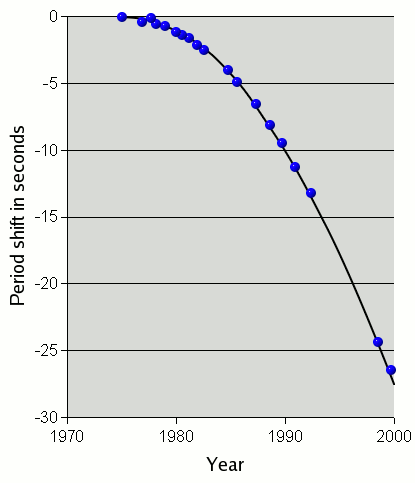
\includegraphics[scale=0.50]{PSR.png}
\caption{The periastron period shift plotted against time, for the Hulse-Taylor PSR1913+16 binary pulsar. The companion arrives earlier at the periastron due to the decrease in separation, hence showing a decrease of the orbital period. Image reproduced from \cite{wikiPSR}}
\label{fig:hulsepulsar}
\end{figure}
  

For the rest of this report, I will concentrate on the first type of source, the coalescing compact binaries, due to the fact that all my work and analysis has been done and will pursue as part of the Compact Binaries Collaboration (CBC), that aims at detecting gravitational waves from this very type of source.



\subsection{Linearized theory of Gravitational Waves produced by a binary system of coalescing compact stars}

Gravitational waves can be naivley seen as {\it ripples} in the
 space-time fabric created by a strong gravitational field source. 
As the first assumptions we consider placing the observer far away from that putative source and 
considering that the gravitational field at the observer is weak but not static,
and that there are no restrictions on the motion of particles in the vicinity of
 the observer. In the absence of gravitational interaction, space-time is flat and
is characterised by the Minkowski flat metric, $\eta_{\mu\nu}={\rm diag}(-1,1,1,1)$. A weak 
gravitational field can be considered as a small 'perturbation' on the
flat Minkowski metric \cite{schutz,maggiore,chaky},

\begin{equation}
\boxed{g_{\mu\nu} = \eta_{\mu\nu} + h_{\mu\nu}, ~~~|h_{\mu\nu}| \ll 1}
\end{equation}

The condition $||h_{\mu\nu}|| \ll 1$ shows that the the analysis is done in a weak gravitational field. Here $||h_{\mu\nu}||$ is defined as the magnitude of a typical non-zero component of $h_{\mu\nu}$. In linearized gravity, the smallness of the perturbation means that
we only keep terms which are linear in $h_{\mu\nu}$, higher order terms are discarded. As
a consequence, indices are raised and lowered using the flat metric $\eta_{\mu\nu}$ . The metric
perturbation $h_{\mu\nu}$ transforms as a tensor under Lorentz transformations. We can therefore write,

\begin{equation}
g^{\mu\nu} = \eta^{\mu\nu} - h^{\mu\nu}
\end{equation}

Under a background Lorentz transformation \cite{schutz}, the perturbation 
transforms as a second-rank tensor:

\begin{equation}
h_{\alpha\beta} = \Lambda_{\alpha}^{~~\mu} \Lambda_{\beta}^{~~\nu} ~h_{\mu\nu}
\end{equation}

The equations obeyed by the perturbation, $h_{\mu\nu}$, are obtained by
writing the Einstein's equations to first order. To the first order, the 
Christoffel symbol is (\cite{schutz,maggiore}),

\begin{equation}
\Gamma^{\lambda}_{~~\mu\nu} = \frac{1}{2} \eta^{\lambda\rho}[\partial_{\mu}
h_{\rho\nu} + \partial_{\nu}h_{\mu\rho} - \partial_{\rho}h_{\mu\nu}] + 
{\cal{O}}(h^2)
\end{equation} 

Therefore, the Riemann curvature tensor will reduce to

\begin{equation}
R_{\mu\nu\rho\sigma} = \eta_{\mu\lambda}\partial_{\rho}\Gamma^{\lambda}_{~\nu\sigma} - \eta_{\mu\lambda}\partial_{\sigma}\Gamma^{\lambda}_{~\nu\rho}
\end{equation}

The Ricci tensor is obtained to the first order as follows:

\begin{equation}
R_{\mu\nu} \approx R^{(1)}_{\mu\nu} = \frac{1}{2}\left[\partial_{\lambda}\partial_{\nu}h^{\lambda}_{~\mu} + \partial_{\lambda}\partial_{\mu}h^{\lambda}_{~nu} - \partial_{\mu}\partial_{\nu}h - \Box h_{\mu\nu}\right]
\end{equation}

where, $\Box = \eta^{\lambda\rho}\partial_{\lambda}\partial_{\rho}$ is 
the D'Alembertian in flat space-time. Contracting with $\eta^{\mu\nu}$,
the Ricci scalar is obtained as follows:

\begin{equation}
R = \partial_{\lambda}\partial_{\mu} h^{\lambda\mu} - \Box h
\end{equation}

The Einstein tensor, $G_{\mu\nu}$, in the limit of weak gravitaty is  (\cite{schutz,maggiore})

\begin{equation}
G_{\mu\nu} = R_{\mu\nu} - \frac{1}{2} \eta_{\mu\nu} R = \frac{1}{2}[\partial_{\lambda}\partial_{\nu}h^{\lambda}_{\mu} + \partial_{\lambda}\partial_{\mu}h^{\lambda}_{~\nu} - \eta_{\mu\nu}\partial_{\mu}\partial_{\nu}h^{\mu\nu} + \eta_{\mu\nu}\Box h - \Box h_{\mu\nu}]
\end{equation}

The Einstein equations read:

\begin{equation}
\boxed{G_{\mu\nu} = R_{\mu\nu} - \frac{1}{2} \eta_{\mu\nu} R = \frac {8 \pi G}{c^4} T_{\mu\nu}}
\label{eqn:einsteinequation}
\end{equation} 

For simplicity one can choose $c=1$. The decomposition (1) of $g_{\mu\nu}$ 
in the weak gravitational field approximation allows for a choice of coordinate systems, not specifying the 
any priviliged system. When one has a system that is invariant
under a gauge transformation, one can fix the gauge and work in a chosen 
coordinate system. One such coordinate system is the Lorentz gauge coordinate system [REF]. 
The gauge condition is called {\it Lorentz gauge}:

\begin{equation}
g^{\mu\nu}\Gamma^{\lambda}_{~~\mu\nu} = 0 
\end{equation}

In the weak field limit, this condition reduces to 

\begin{equation}
\partial_{\lambda} h^{\lambda}_{~~\mu} = \frac{1}{2}\partial_{\mu} h
\end{equation}

In this chosen gauge, the linearized Einstein equations simplify to:

\begin{equation}
\Box h_{\mu\nu} - \frac{1}{2} \eta_{\mu\nu}\Box h = - 16 \pi G T_{\mu\nu}
\end{equation}

The trace-reversed perturbation, $\bar{h}_{\mu\nu}$, is defined as follows (\cite{schutz,maggiore,chaky}):

\begin{equation}
\bar{h}_{\mu\nu} = h_{\mu\nu} - \frac{1}{2}\eta_{\mu\nu} h
\end{equation}

The Lorentz gauge condition further reduces to:

\begin{equation}
\partial_{\mu} \bar{h}^{\mu}_{~\lambda} = 0
\end{equation}

The Einstein equations are then (\cite{schutz,maggiore}):

\begin{equation}
\Box \bar{h}_{\mu\nu} = - 16 \pi G T_{\mu\nu}
\end{equation}

The above equation is written in the presence of matter and energy. If written in vacuum, 
where the stress-energy tensor will vanish, we obtain the familiar plane waves equation:

\begin{equation}
\Box \bar{h}_{\mu\nu} = 0
\end{equation}

The vacuum equations for $\bar{h}_{\mu\nu}$ are similar to the wave 
equations in electrodynamics or acoustics. 
These second order partial differential equations will have plane-wave solutions of the type (\cite{schutz,maggiore,chaky,ian}):

\begin{equation}
\bar{h}_{\mu\nu} = B_{\mu\nu} {\rm exp}(i k_{\alpha}x^{\alpha})
\end{equation}

where, $B_{\mu\nu}$ is a constant, symmetric second rank tensor and $k_{\alpha}$
is a constant four-vector known as the {\it plane wave vector}. The waves are propagating 
with a group velocity $c=1$ and the dispersion relation will be:

\begin{equation}
\omega^2 = |{\bf k}|^2
\end{equation}

Using the Lorentz gauge condition 
(14), one obtains as follows:

\begin{equation}
k_{\alpha} B^{\alpha\beta} = 0 
\end{equation}

This imposes a restriction on $B^{\alpha\beta}$ : it is orthogonal 
({\it transverse}) to $k_{\alpha}$. 
It can be easily proved that any coordinate transformation of the form

\begin{equation}
x^{\alpha^{\prime}} = x^{\alpha} + \xi^{\alpha}(x^{\beta})
\end{equation}

will leave the plane wave equation

\begin{equation}
\Box x^{\mu} = 0
\end{equation}

satisfied as long as

\begin{equation}
\Box \xi^{\alpha} = 0
\end{equation}

One can therefore choose a solution (\cite{chaky})

\begin{equation}
\xi_{\alpha} = C_{\alpha} {\rm exp}(i k_{\beta} x^{\beta})
\end{equation}

to the wave equation for any $\xi_{\alpha}$. $C_{\alpha}$ are constant 
coefficients. If

\begin{equation}
B^{\mu}_{\mu} = 0 ~~~~({\rm \it traceless})
\end{equation}

and

\begin{equation}
B_{\mu\nu} V^{\beta} = 0
\end{equation}

where, $V^{\beta}$ is some fixed four-velocity, that is, any constant 
time dependent unit vector one wishes to choose. The equations

\begin{equation}
\boxed{k_{\alpha} B^{\alpha\beta} = 0 \hspace{1cm}
B^{\mu}_{\mu} = 0 \hspace{1cm}
B_{\mu\nu} V^{\beta} = 0}
\end{equation}

 are called the the {\it transverse traceless} (TT) gauge 
conditions (\cite{schutz,maggiore,ian,chaky}). The trace condition $B^{\mu}_{\mu} = 0$ implies that

\begin{equation}
\bar{h}^{TT}_{\alpha\beta} = h^{TT}_{\alpha\beta}
\end{equation}

Consider now a background Lorentz transformation in
which the vector $V^{\alpha}$ is the time basis vector $V^{\alpha} = 
\delta^{\alpha}_{~0}$. Then the third TT equation implies that $B_{\mu 0} = 0$ for all
$\mu$ (\cite{maggiore,chaky}). 

Consider now a priviliged orientation of the coordinate axes so that the wave is travelling 
along the $z$-direction, $k^{\mu} \rightarrow (\omega, 0, 0, \omega)$. 
Then with the TT equations it implies that $B_{\alpha z} = 0$ for all
$\alpha$. Thus, $B^{TT}_{\alpha\beta}$ in matrix form is 

\begin{equation}
B^{TT}_{\alpha\beta} = \left( \begin{array}{cccc}
              0 & 0 & 0 & 0 \\
              0 & B_{xx} & B_{xy} & 0 \\
              0 & B_{xy} & -B_{xx} & 0 \\
              0 & 0 & 0 & 0 \end{array} \right)
\end{equation}

The $xx$ and $xy$ components of the amplitude tensor are also called the polarizations and labelled as $xx \equiv +$ and $xy \equiv \times$ as in the following (\cite{schutz,maggiore,chaky,ian}):

\begin{equation}
\boxed{B^{TT}_{\alpha\beta} = \left( \begin{array}{cccc}
              0 & 0 & 0 & 0 \\
              0 & B_+ & B_{\times} & 0 \\
              0 & B_{\times} & -B_{+} & 0 \\
              0 & 0 & 0 & 0 \end{array} \right)}
\label{eqn:polarizations}
\end{equation}
 
To obtain the solution of the linearised wave equations, the Green's function method will be used (\cite{schutz,maggiore,chaky}).
The Green's function, $G(r_1 - r_2)$, of the D'Alembertian 
operator $\Box$, is the solution of the wave equation in the presence of 
a delta function source:

\begin{equation}
\Box~G(r_1 - r_2) = \delta^{(3)}(r_1 - r_2)
\end{equation}

where $\delta^{(3)}$ is the three-dimensional Dirac delta function (stepped over time) (\cite{schutz,maggiore,chaky}). The 
general solution to the linearized Einstein's equations can be 
written using the Green's function as


\begin{equation}
\bar{h}_{\mu\nu}(t, {\bf r_1}) = 4G\int d^3 {\bf r}_2~\frac{1}{|{\bf r}_1 - {\bf r}_2|}
T_{\mu\nu}(t - |{\bf r}_1 - {\bf r}_2|, {\bf r}_2) 
\end{equation}

The quantity

\begin{equation}
t_{\rm r} = t - |{\bf r}_1 - {\bf r}_2|
\end{equation}

is called the {\it retarded time} with ${\bf D}= {\bf r}_1- {\bf r}_2$. From the expression for $\bar{h}_
{\mu\nu}$, it is easy to observe that the perturbation in the gravitational field at 
$(t, {\bf r}_1)$ is a sum of the influences from the energy and momentum 
sources at the point $(t_{\rm r}, {\bf r}_2)$.

One can now considers the gravitational radiation
emitted by an isolated far away source consisting of very slowly moving 
particles (the spatial dimensions of the source are neglected compared 
to the distance between the source and the observer) (\cite{maggiore,chaky}). The Fourier 
transform of the perturbation $\bar{h}_{\mu\nu}$ is 

\begin{equation}
{\tilde{\bar{h}}}_{\mu\nu} (\omega, {\bf r}_1) = \frac{1}{\sqrt{2\pi}}\int {\rm d}t~{\rm exp}
(i\omega t)~\bar{h}_{\mu\nu}(t, {\bf r}_1)
\end{equation}

Using the expression for $\bar{h}_{\mu\nu} (t, {\bf r}_1)$, one obtains

\begin{equation}
{\tilde{\bar{h}}}_{\mu\nu} = 4G\int {\rm d}^3 {\bf r}_2 ~{\rm exp}(i\omega |{\bf r}_1 - 
{\bf r}_2|)~\frac{\tilde{T}_{\mu\nu}(\omega, {\bf r}_2)}{|{\bf r}_1 - {\bf r}_2|}
\end{equation}

Under the assumption that the spatial extent of the source is much smaller
compared to the distance between the source and the observer (\cite{maggiore,chaky,ian}), one can replace
the term ${\rm exp}(i\omega |{\bf r}_1 - {\bf r}_2|)/|{\bf r}_1 - {\bf r}_2|$ 
in by ${\rm exp}(i\omega{\rm D})/{\rm D}$. Therefore,

\begin{equation}
\tilde{\bar{h}}_{\mu\nu}(\omega, {\bf r}_1) = 4G~\frac{{\rm exp}(i\omega
{\rm D})}{{\rm D}}~\int {\rm d}^3 {\bf r}_2~\tilde{T}_{\mu\nu}(\omega, {\bf r}_2)
\end{equation}

The Lorentz gauge condition in Fourier space is 

\begin{equation}
\partial_{\mu}\bar{h}^{~\mu\nu}(t, {\bf r}_1) = \partial_{\mu}\int {\rm d}\omega~
{\tilde{\bar{h}}}^{~\mu\nu}~{\rm exp}(-i\omega t) = 0
\end{equation}

Separating out the space and time components, using Gauss' theorem (\cite{maggiore,chaky}): 

\begin{equation}
\int {\rm d}^3 {\bf r}_2~\tilde{T}^{ij}(\omega, {\bf r}_2) = - \int {\rm d}^3 {\bf r}_2~r_2^{i} \left(\partial_k \tilde{T}^{kj}\right)
\end{equation}	

and considering the Fourier space version of the conservation of energy equation for 
$T^{\mu\nu}$, that is, $\partial_{\mu} T^{\mu\nu}(t, {\bf r}_1) = 0$ and finally introducing the {\it quadrupole moment tensor} (\cite{schutz,maggiore,chaky,ian}) of the energy-density of the source as

\begin{equation}
\tilde{Q}_{ij}(\omega) = \int {\rm d}^3 {\bf r}_2~r^{i}r^{j}~\tilde{T}^{00}(\omega, {\bf r}_2)
\end{equation}

With respect of the newly defined quadrupole moment tensor, we have

\begin{equation}
\int {\rm d}^3 {\bf r}_2~\tilde{T}^{ij}(\omega, {\bf r}_2) = - \frac{\omega^2}{2}~
\tilde{Q}_{ij}(\omega)
\end{equation}

Hence, the solution reads

\begin{equation}
\tilde{\bar{h}}_{ij}(\omega, {\bf r}_1) = 4G~\frac{{\rm exp}(i\omega{\rm D})}
{{\rm D}}\left(-~\frac{\omega^2}{2}\tilde{Q}_{ij}(\omega)\right)
\end{equation}

and making further simplifications,

\begin{equation}
\tilde{\bar{h}}_{ij}(\omega, {\bf r}_1) = -2~\frac{G\omega^2}{{\rm D}}
~{\rm exp}(i\omega{\rm D})~\tilde{Q}_{ij}(\omega)
\end{equation}

The final expression of the metric perturbation is obtained after a last Fourier transform (\cite{chaky}):

\begin{equation}
\bar{h}_{ij}(t, {\bf r}_1) = \frac{2G}{{\rm D}}~\frac{{\rm d}^2}{{\rm d}t^2}~Q_{ij}(t_{{\rm r}})
\end{equation}

where, $t_{{\rm r}} = t - |{\bf r}_1 - {\bf r}_2|=t - D$ is the retarded time. To write this expression in SI units:

\begin{equation}
\boxed{\bar{h}_{ij}(t, {\bf r}_1) = \frac{2G}{c^4{\rm D}}~\frac{{\rm d}^2}{{\rm d}t^2}~Q_{ij}(t - \frac {|{\bf r}_1 - {\bf r}_2|}{c})}
\label{eqn:inertia}
\end{equation}

To get a more general solution, we need to remove the $z$ propagation condition. To obtain the new expression for 
$\bar{h}_{ij}(t, {\bf r}_1)$ we need to apply a rotation ${\rm \bf R}={\rm \bf R}(\theta, \phi)$ matrix with the new
quadrupole moment defined as (\cite{maggiore,ian})

\begin{equation}
Q_{ij}^r = {\rm \bf R}^T(\theta, \phi)~Q_{ij}~{\rm \bf R}(\theta, \phi)
\end{equation}

While higher order multipole moments of the mass distribution can contribute to the radiation, for most systems the quadrupole will dominate. Further, the mass monopole and dipole moment will not contribute any gravitational waves. Thus, such events as a spherically symmetric gravitational collapse and axially symmetric rotation do not emit any gravitational radiation (\cite{maggiore,cre}) . On the other hand, a rotating dumbell is an excellent emitter of gravitational waves, making binary systems potentially amongst the brightest emitters of waves in the Universe.

Two compact stars (binary neutron stars, neutron star-black hole or binary black holes) orbit each other in a 
close orbit and due to the very strong gravitational field produced by this high-mass system, gravitational waves are emitted. By emitting gravitational waves, the system loses energy and angular momentum hence the separation between the objects lessens with every orbit. The closer the stars get to each other, more orbital energy is converted into gravitational waves, hence, the stronger the gravitational waves are. This system can be easily modelled analytically, in a Newtonian approximation, as described below. 

Let´s consider such a system of two inspiralling compact objects, orbiting each other around the common 
center of mass (CM). The components have masses $m_1$ and $m_2$, orbiting with an angular velocity $\Omega=\Omega(t)$ and the orbit is considered plane circular and obeying the classical keplerian laws for celestial bodies. The system can be considered in quasi-equilibrium  at the time $t$ much smaller than the coalescence time if (\cite{maggiore})

\begin{equation}
\frac {{\rm d} \Omega(t)}{{\rm d}t} \ll \Omega^2(t)
\end{equation}
where $\Omega=\Omega(t)$ is the orbital frequency.

The separation $r=r(t)$ between the stars will decrease gradually and reach null value at merger. In plane, carthesian coordinates, the system is described by the position coordinates with respect to CM:

\begin{equation}
x_1(t) = r \cos (\Omega t+ \phi_0) \hspace{10mm}
x_2(t) = r \sin (\Omega t+ \phi_0) \hspace{10mm}
x_3(t)=0
\end{equation}

In the center of mass of the system the moment of inertia (the second mass moment) is (\cite{maggiore,ian})

\begin{equation}
Q^{ij} = \mu~x^i(t)~x^j(t)
\end{equation}

where $\mu=m_1m_2/(m_1+m_2)$ is the reduced mass. Taking the time derrivatives and applying equations \ref{eqn:polarizations} and \ref{eqn:inertia} we calculate $h_{ij}=(h_+, h_{\times})$ for the system. It is convenient to introduce the {\it chirp} {\it mass} as follows:

\begin{equation}
 M_c= \frac{{(m_1m_2)}^{3/5}}{{(m_1+m_2)}^{1/5}}
\label{eqn:chirpmass}
\end{equation}


A solution of equation (43) in a geocentric reference frame would read (\cite{maggiore}):

\begin{equation}
\boxed{h_+(t) = \frac{4}{D} ~\left({\frac{GM_c}{c^2}}\right)^{5/3}~\left[{\frac{\pi f_{gw}(t)}{c}}\right]^{2/3}~ \frac{1+\cos^2 \theta}{2}~ \cos(2 \pi f_{gw}t_{ret}+2 \phi)}
\label{eqn:hplus}
\end{equation}

\begin{equation}
\boxed{h_{\times}(t) = \frac{4}{D} ~\left({\frac{GM_c}{c^2}}\right)^{5/3}~\left[{\frac{\pi f_{gw}(t)}{c}}\right]^{2/3}~ \cos \theta~\sin (2 \pi f_{gw}t_{ret}+2 \phi)}
\label{eqn:hcross}
\end{equation}

where $f_{gw}=\omega_{gw}/2 \pi=2\Omega/2 \pi$ is the frequency of the gravitational wave (double the orbital frequency) and $t_{ret} \equiv t-D/c$ is the retarded time. The waveforms consist of a time-varying amplitude and a time-varying phase for the two polarizations:

\begin{equation}
A_+ (t) = \frac{4}{D} ~\left({\frac{GM_c}{c^2}}\right)^{5/3}~\left[{\frac{\pi f_{gw}(t)}{c}}\right]^{2/3}~ \frac{1+\cos^2 \theta}{2} 
\end{equation}

\begin{equation}
\Phi_+(t) = \Phi_{\times}(t) = 2 \pi f_{gw}(t)t_{ret}(t)+2 \phi
\end{equation}

\begin{equation}
A_{\times} = \frac{4}{D} ~\left({\frac{GM_c}{c^2}}\right)^{5/3}~\left[{\frac{\pi f_{gw}(t)}{c}}\right]^{2/3}~ \cos \theta
\end{equation}

The gravitational waves emmission causes the loss of orbital energy hence the orbits become shorter with time, the orbital frequency increasing. The gravitational wave will chirp reaching its maximum amplitude and frequency at the merger of the two stars. Considering th equilibrium between the loss of orbital energy and the gain in gravitational energy one can write down the energy conservation law (\cite{maggiore})

\begin{equation}
P_{gw} = \frac {{\rm d}E_{gw}}{{\rm d}t} =  \frac {32}{5}~ \frac {c^5}{G}~\frac{{(GM_c \omega_{gw}(t))}^{10/3}}{2^{10/3}~c^{10}}
\end{equation}

and

\begin{equation}
P_{orbit} = \frac {{\rm d}E_{orbit}}{{\rm d}t} = - \frac {{\rm d}}{{\rm d}t}~ \frac{G^{2/3}M_c^{5/3}\omega_{gw}^{2/3}(t)}{{32}^{1/3}}
\end{equation}

Placing $P_{gw} = P_{orbit}$ we can solve for $\omega_{gw}=\omega_{gw}(t)$ and obtain, after a series of calculations (\cite{maggiore,ian}):

\begin{equation}
\boxed{\omega_{gw}(\tau) = \frac {1}{4}~\left({\frac {\tau}{5}}\right)^{-3/8}~ \left({\frac{GM_c}{c^3}}\right)^{-5/8}}
\end{equation}

where $\tau \equiv t-t_{coal}$ is the time to coalescence. The shape of the wave is pictured in Figure ~\ref{fig:chirp}(\cite{ligoweb}) and represents the newtonian approximation in linear orders of $v/c$ for the inspiral phase, in other words in weak gravity.  

\begin{figure}[ht]
\centering
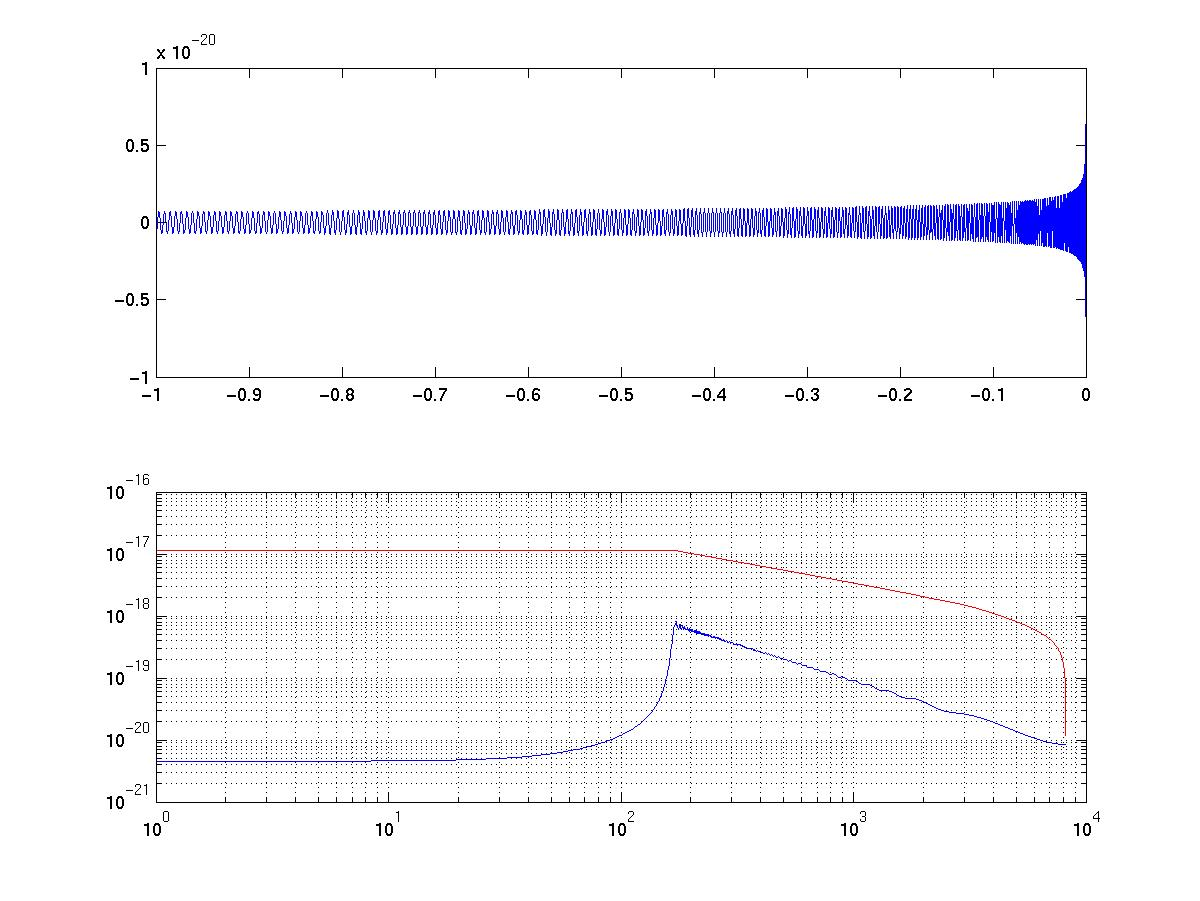
\includegraphics[scale=0.25]{chirpfreq.jpg}
\caption{Chirp gravitational wave from a typical coalescence of two inspiralling compact stars: the figure on top shows the time dependency of either $h_+$ or $h_{\times}$ and the figure on the bottom shows the time dependency of the GW frequency (blue curve) and its integral (red curve). The figure is reproduced from \cite{ligoweb}}
\label{fig:chirp}
\end{figure}

\section{Detectors of Gravitational Waves}

There is variety in the types of gravitational waves detectors in use nowadays. The most widely used and altogether the largest type of detector uses laser light intereferometry as functional principle. A simplified schematic of a Michelson laser interferometry GW detector is pictured in Figure ~\ref{fig:detector}.

\begin{figure}[ht]
\centering
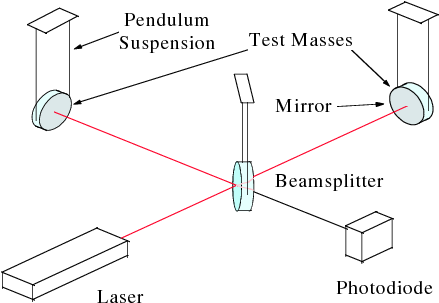
\includegraphics[scale=0.30]{detector.png}
\caption{Schematics of a Michelson interferometer. Image reproduced from \cite{ligoweb,ian}}
\label{fig:detector}
\end{figure}

It consists of two arms oriented at a 90 degree angle with laser beams running along the length of the arms. The laser light is emitted at the centre of the “L” shape and split using a beam splitter, the light then travels along each of the arms, is reflected by mirrors at the end of each arm, passes back down along the arms and is recombined
at the initial starting point. The principle is that as the path length for the light to travel down the arms
varies, the laser light being recombined will have a variable phase difference and thus by
observing the interference pattern we can measure the change in path length between
the two arms. 

Consider now an $O$-shaped string of test masses subject to the passage of a gravitational wave $h(t)=(h_+, h_{\times})$. The effect of the $+$ polarization is shown in Figure ~\ref{fig:massesplus} and the effect of the $\times$ polarization is shown in Figure ~\ref{fig:massescross} [REF].
The gravitational wave, when passing through the interferometer, will alter the lengths of the light arms (paths) just as the particles separation is altered in Figure ~\ref{fig:massesplus} and Figure ~\ref{fig:massescross}. By changing the lengths of the light paths one can get an interference pattern at the recombination point. 

\begin{figure}[ht]
\begin{minipage}[b]{0.5\linewidth}
\centering
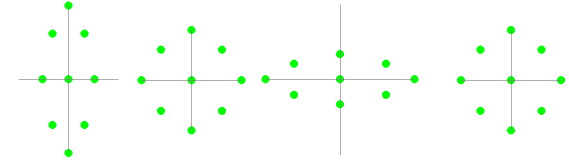
\includegraphics[scale=0.35]{plus.png}
\caption{Effect of passage of $+$ polarization. Image reproduced from \cite{ian}}
\label{fig:massesplus}
\end{minipage}
\hspace{0.5cm}
\begin{minipage}[b]{0.5\linewidth}
\centering
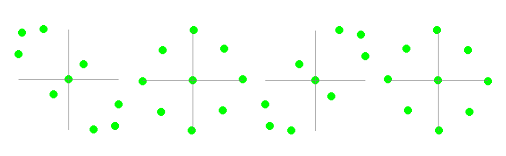
\includegraphics[scale=0.35]{cross.png}
\caption{Effect of passage of $\times$ polarization. Image reproduced from \cite{ian}}
\label{fig:massescross}
\end{minipage}
\end{figure}

\paragraph{LIGO}(\cite{ligoweb,LIGOIFO,LLOweb,LHOweb,abbott2006,abbott2007,ian,cre}) The Laser Interferometry Gravitational Observatory (LIGO) is the largest interferometer in use as of today. LIGO operates two gravitational wave observatories in unison: the LIGO Livingston Observatory in Livingston, Louisiana and the LIGO Hanford Observatory, located near Richland, Washington. These sites are separated by 3,002 kilometers [REF]. Since gravitational waves are expected to travel at the speed of light, this distance corresponds to a difference in gravitational wave arrival times of up to ten milliseconds. Each observatory supports an L-shaped ultra high vacuum tubes system, measuring 4 kilometers on each side. The primary interferometer at each site consists of mirrors suspended at each of the corners of the L; it is known as a special Michelson interferometer in that it recycles the power. A pre-stabilized laser emits a beam of up to 35 W that passes through a beam splitter at the vertex of the L. There, the beam splits into two paths, one for each arm of the L; each arm contains special cavities that store the beams and increase the effective path length by multiple reflections.

When a gravitational wave passes through the interferometer, the space-time in the local area is altered. Depending on the source of the wave and its polarization, this results in an effective change in the length of one or both of the L cavities. This length change will bring the cavity very slightly out of resonance, and will cause the in the cavity to slightly change its phase compared to the incoming light.

After an equivalent of approximately 75 trips up and down the 4 km length to the far mirrors and reverse, the two separate beams leave the arms and recombine at the beam splitter. The beams returning from two arms are kept out of phase so that when the arms are both in resonance (as when there is no gravitational wave passing through), their light waves subtract, and no light should arrive at the photodiode. When a gravitational wave passes through the interferometer, the distances along the arms of the interferometer are shortened and lengthened, causing the beams to become slightly less out of phase, so that some light arrives at the photodiode, indicating a signal. The $h = \delta l/l$ is actually measured in this way, with $\delta l/l$ the relative variation in length of the detector arms due to the passage of the gravitational wave and $h$ the amplitude of the GW. A detector with an arm length of 4 km responds to a gravitational wave with an amplitude of $10^{-21}$ due to an actual variation in length of about $\delta l=4 \times 10^{-18}$ m-this is actually the order of magnitude of the size of an atom.

In the case of a ground-based laser interferometer like LIGO, in the time-domain, $h=h(t)$ can be written as a linear combination of its two polarizations $h_{\times}$ and $h_+$ given in equations Equation ~\ref{eqn:hplus} and Equation ~\ref{eqn:hcross} (\cite{ligoweb,LIGOIFO,LLOweb,LHOweb,abbott2006,abbott2007,maggiore}):

\begin{equation}
 h(t)=F_{\times}h_{\times}+F_+h_+
\end{equation}

where  $F_{\times}$ and $F_+$ are the so-called antenna factors that are functions of $(\theta, \phi)$, the position angles on the sky, of the binary. These two functions appear in the waveform due to purely geometrical reasons: they are introduced when rotating the reference system of the wave onto the refenece system of the detector. They are known for each binary system analyzed and their RMS tells us how the binary is oriented with regards to the detector. Ideally we would expect an RMS equal to 1 for a perfect overhead orientation ($F_+$=1 and $F_ \times$=0). Their expressions in terms of $\theta$ and $\phi$ are given below (\cite{abbott2006,abbott2007,maggiore}):

\begin{equation}
F_+(\theta, \phi) = \frac{1}{2}(1+\cos^2 \theta)\cos(2 \phi)
\end{equation}

\begin{equation}
F_{\times}(\theta, \phi) = \cos \theta \sin(2 \phi)
\end{equation} 

With such small detected signals, noise plays an important role. The main sources of noise for a typical LIGO-like detector are given in (\cite{ligoweb,LIGOIFO,LLOweb,LHOweb,abbott2006,abbott2007,maggiore}):

\begin{itemize}
 \item
   {\bf Thermal noise} Thermal vibrations of the internal parts of the interferometer
can mask gravitational waves. Interferometers minimise the effect of
noise by measuring only at frequencies far from the resonant frequency,
and making sure all materials have high quality factors, so their resonances are sharp
and energy leakage to measurement frequencies is small. In terms of temperature, interferometers usually
operate at room temperature.
 \item
   {\bf Shot noise} The photons that are used to do interferometry are quantized,
and so they arrive with random phases and hence make random
fluctuations in the interference pattern that can look like a gravitational
wave signal. The more photons one uses, the smoother will be the interference
signal.
  \item
  {\bf Ground vibration} Mechanical vibrations must be screened out. There
are many different ways to do this, but all of them are very sensitive to
frequency, working well down to a lowest effective frequency. The most
ambitious isolation system is being developed for the Virgo detector. The third generation detectors (LISA) will
be space based so this problem is eliminated.
\end{itemize}

A sensitivity curve for a detector, or a noise curve, represents an $n=n(f)$ plot where $n$ is the detector noise and such a set of curves is pictured in Figure ~\ref{fig:ligonoise} for the LIGO observatory (\cite{ligoweb,LIGOIFO,abbott2006,abbott2007}):

\begin{figure}[ht]
\centering
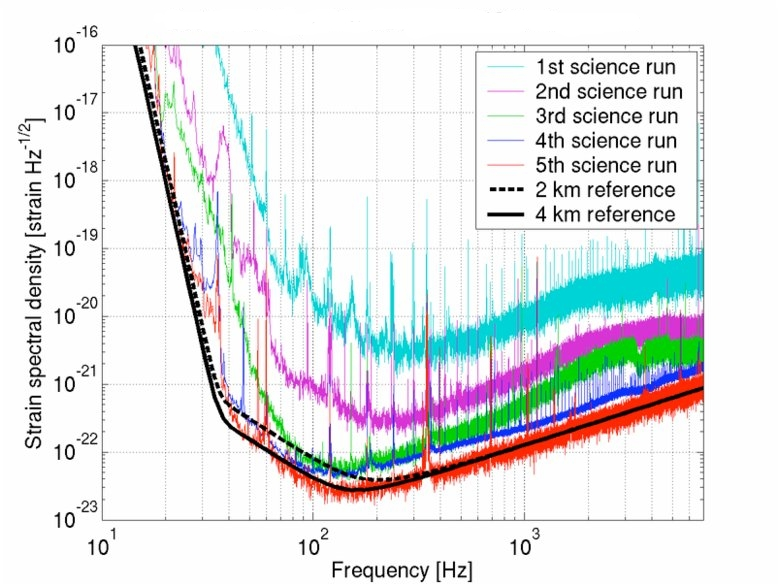
\includegraphics[scale=0.30]{ligonoise.jpg}
\caption{LIGO noise curve for five different science runs (\cite{abbott2006,abbott2007,ligoweb,ian})}
\label{fig:ligonoise}
\end{figure}


\section{Data Analysis Procedures}

\subsection{Matched Filtering}

Firstly we will (re-)introduce the Fourier transform of a function of time $F(t)$ as denoted by
$\tilde F (f)$ and is given by (\cite{allen,maggiore,cre}):

\begin{equation}
{\tilde F}(f) = \int {\rm e}^{- 2 \pi i f t} F(t) dt.
\end{equation}

The inverse Fourier transform will be converseley

\begin{equation}
F(t)= \int {\rm e}^{2 \pi i f t} {\tilde F}(f) df.
\end{equation}

The typical gravitational wave detector output is denoted by

\begin{equation}
s(t) = n(t) + h(t)
\end{equation}

where $n(t)$ is the (real) strain-equivalent noise produced by
fluctuations within the detector due to external and internal mechanical causes, and $h(t)$ is a
 gravitational waveform of astrophysical origin.

The detector´s noise can not be controlled or analytically generated in any way. It is purely a consequence of 
the internal vibrations of the detector´s components (e.g. mirrors) and of the external vibrations due to 
environmental factors (earthquakes, passing trucks etc). There are different data channels in the detectors that monitor noise only and a lot of the spurious effects of internal and external noise are vetoed. Thus, the detector's noise $n(t)$ can only be characterized
statistically by sampling the noise data and building a noise power spectrum. For simplicity of calculations we will assume that the noise is Gaussian and stationery. This is actually close to the real case, minus the accidental peaks (glitches) that escape the veto tests. 
One must introduce tools for determining the expected
properties of quantities measured in the presence of this noise.
One can assume that $n(t)$ is a random time-series drawn from a large
ensemble of such time series, and that $\langle n(t) \rangle $ vanishes, which implies that
$\langle \tilde n(f) \rangle =0$ (white noise). This implies that the
expectation value $\langle n(t) n(t') \rangle$ depends only upon the
time difference $|t-t'|= \tau$ (\cite{allen,maggiore,cre}). It then follows that in frequency space

\begin{equation}
\langle \tilde n(f) \tilde n^*(f') \rangle = \frac{1}{2}~ S_n(f) \delta(f-f'),
\end{equation}

where $\delta(f)$ is the Dirac delta-function in frequency space and the real non-negative even function $S_n(f)$ is the noise power spectral density (PSD).

The search method applied is {\it matched filtering}(\cite{allen,maggiore,cre,abbott2007}): the gravitational waveform is known apriori and expected in the detector´s output, together with noise, hence, equal segments of output data and expected signal are treated as vectors and the degree of overlapping of the two vectors is given by a linear filter, or a hermitian inner product.  
We can consider the detector output $s(t)$ and a signal $h(t)$ that
lasts for a duration of $T$.  If the signal arrives at the detector at time
$t_0$, then the detector output can be written
\begin{equation}
    s(t)=\left\{  
    \begin{array}{lc}
        h(t-t_0)+n(t), ~ ~ ~ ~ ~& t_0<t<t_0+T\\
        n(t), & \mbox{otherwise}
    \end{array}
    \right. 
    \label{eq:h(t)}
\end{equation}
where $n(t)$ is the detector noise. Introducing the filter function $K(t)$ in the time domain, the filtered output signal $S$ will be 

\begin{equation}
S = {\int}_{-{\infty}}^{\infty}\, K(t) \langle s(t) \rangle ~dt = {\int}_{-{\infty}}^{\infty}\, K(t) h(t) ~dt = {\int}_{-{\infty}}^{\infty}\, \tilde K^*(f) \tilde h(f)~df
\end{equation}

and the noise will be

\begin{equation}
N^2 = {\int}_{-{\infty}}^{\infty}\,{\int}_{-{\infty}}^{\infty}\, K(t)K(t+ \tau) \langle n(t)n(t+ \tau) \rangle ~dt ~d \tau = {\int}_{-{\infty}}^{\infty}\, \frac {1}{2} S_n(f) {|\tilde K(f)|}^2~df
\end{equation}

The signal to noise ratio is defined as SNR={\it S/N} and the question arises which is the filter function that maximizes the SNR? By introducing a hermitian inner product between two vecors $A$ and $B$ as in (\cite{allen,maggiore}) 

\begin{equation}
(A|B) = 4 {\rm Re} {\int}_0^{\infty}\, \frac {\tilde A^*(f) \tilde B(f)}{S_n(f)}~df
\end{equation}

we observe that the SNR can be written in a compact way as:

\begin{equation}
S/N = \frac {(s|h)}{\sqrt {(h|h)}}
\end{equation}

and if the filter function is expressed as

\begin{equation}
\tilde K(f) = {\rm const.}~\frac {\tilde h(f)}{S_n(f)}
\end{equation}

the SNR is maximized to 

\begin{equation}
{(S/N)}_{\rm {max}} = \sqrt {(h|h)}
\end{equation}

The waveforms $h(t)$ depend on a series of parameters: $h=h(m_1,m_2,d,s_1,s_2, \iota, \theta, \phi, \Phi_0, t_0,f_{gw}(t))$ where $m_{1,2}$ are the masses of the two binary components, $d$ is the distance from the binary centre of mass, $s_{1,2}$ are the spins of the binary components, $\iota$ is the inclination of the binary with respect to the line of sight, $\theta$ and $\phi$ are the position angles on the sky (right ascension and declination), $\Phi_0$ and $t_0$ are the coalescence phase and time, $f_{gw}(t)$ is the GW frequency as a function of time. Since these parameters are a continuous series, it is not possible to search at every possible parameter value for each of the
binary components. However, if a signal is close enough to a template, the loss of SNR will be small. Thus, by using an appropriate set of
templates, called a \emph{template bank} in mass space, one can cover all masses in the
desired mass interval with some predetermined maximum loss in SNR. The smaller the maximum loss in SNR, the
larger the number of templates needed in the bank [REF]. Typically, searches will
implement a template bank with a maximum SNR loss of 3 percent, which leads to
template banks containing of the order of a few hundred templates (the exact
number depends on the noise spectrum).

\subsection{$\chi^2$ test}(reference for this subsection is \cite{allen,maggiore,cre}) 

When noise is Gaussian and stationery the matched filtering technique gives the best probability to find a signal with a before-known waveform. Most of the times, though, the detector noise contains very energetic peaks (noise glitches) that affect somtimes the template bank by it rendering a high SNR to these glitches. It is necessary to have some other way of distinguishing the majority of glitches from true signals.

The method which has become standard for this is to use a \emph{chi-squared}
(${\chi}^2$) veto test [REF]. When a template exceeds a certain threshold SNR, 
it is then divided into $p$ different frequency bands such
that each band should yield $1/p$ of the total SNR of the data if the high SNR
event was a signal matching the template. The sum of the squares of the
differences between the expected SNR and the actual SNR from each of the $p$
bands, that is the ${\chi}^2$ statistic, is then calculated. The advantage of
using the ${\chi}^2$ veto is that glitches tend to produce large ${\chi}^2$ values, 
and are therefore distinguishable from true gravitational waves
signals. Thus, only those template matches with low enough ${\chi}^2$ values
are considered triggers. 

If the data was a matching signal in Gaussian noise, the ${\chi}^2$ statistic
would be ${\chi}^2$ distributed with $2p-2$ degrees of freedom
[REF].  However, it is much more likely that the template that
produces the highest SNR will not be an exact match for the signal. In this
case, denoting the fractional loss in SNR due to mismatch by ${\mu}$, the
statistic is distributed as a non-central chi-squared, with non-centrality
parameter ${\lambda}\,{\leq}\,2{\varrho}^2{\mu}$.  This simply means that
the ${\chi}^2$ threshold, ${\chi}^*$, depends quadratically on the measured
SNR, ${\varrho}$, as well as linearly on $\mu$.   

\section{Short Hard Gamma Ray Burst GRB070429B analyzed by the inspiral pipeline}

Gamma-ray bursts ({\it GRB}) are the most luminous electromagnetic events occurring in the universe since the Big Bang. They are flashes of gamma rays emanating from seemingly random places in deep space at random times. The duration of a gamma-ray burst is typically a few seconds, but can range from a few milliseconds to several minutes, and the initial burst is usually followed by a longer-lived afterglow emitting at longer wavelengths (X-ray, ultraviolet, optical, infrared, and radio). Gamma-ray bursts are detected by orbiting satellites (e.g. SWIFT, BATSE) about two to three times per week. Most observed GRBs appear to be collimated emissions caused by the collapse of the core of a rapidly rotating, high-mass star into a black hole. A subclass of GRBs (the {\it short} bursts) appear to originate from a different process, the leading theory being the merger of neutron stars orbiting in a binary system and are characterized by a much harder $\gamma$ spectrum and a shorter burst time. Until 2007, only a handful of these events have been localized to a definite galactic host (\cite{nakar}). However, those that have been localized appear to show significant differences from the long-burst population. While at least one short burst has been found in the star-forming central region of a galaxy, several others have been associated with the outer regions and even the outer halo of large elliptical galaxies in which star formation has nearly ceased. All the hosts identified so far have also been at low redshift (\cite{nakar}). Furthermore, despite the relatively nearby distances and detailed follow-up study for these events, no supernova has been associated with any short GRB (\cite{nakar}).


\subsection{Introducing GRB070429B}

GRB070429B was a short hard $\gamma$-ray burst that was observed on April 29, 2007 at 03:09:04 by the Swift/UVOT sattelite. Its duration was 0.500 s and its sky location was RA 328.02 and DEC -38.84.LIGO's operational IFO's at the time of the GRB were Hanford 1 (H1) and Livingston (L1). What is interesting to note is that the antenna factors $F_{\times}$ and $F_+$ for H1 and L1 are 0.99 and 0.93 respectivley giving an $F_{RMS}$ equal to 0.96 which reveals an almost overhead position with respect to H1L1.Both H1 and L1 detectors were running in science mode at the time of the GRB. 
The astronomical and detector data summarizing the characteristics of GRB070429B is presented in Table 1. 

\begin{table}[ht]
 \begin{tabular}{|l|l|l|l|l|l|l|l|l|}
 \hline
 \hline
 GPS & Date & redshift & duration [s] & RA & DEC & H1 & H2 & L1 \\
 \hline
 861851358 & Apr 29 2007 03:09:04 & 0.904 & 0.43 & 328.02 & -38.84 & 0.99 & 0.99 & 0.93 \\
 \hline
 \hline
 \end{tabular} 
 \caption{Astronomical and detector data for GRB070429B}
 \label{Table 1}
\end{table}

 It is interesting to note that initially, in the GRB data record that LIGO is using, there was no redshift associated with this particular GRB. Nevertheless, at a closer look at the GCN circulars written on GRB070429B a possible redshift can be assigned by association with a faint object (galaxy) seen on the night of October 9, 2007, using the Keck telescope. Longslit measurements have been performed and the trace of object was found to be faint and the spectrum was mostly featureless, but a faint line signature was observed centered at 7098 Angstroms. The feature was identified as most likely being the [OII] 3727 doublet. Other line identifications ($H-\alpha$, $H-\beta$, or [OIII]) were disfavored due to the absence of corroborating lines that would be expected over the spectral range (3500-8900 Angstroms) in those cases. Association of this feature with [OII] indicates a redshift for this object of z=0.904 (luminosity distance of about 4 Gpc). Calibrating relative to R-band photometry, the estimate was a preliminary line flux corresponding to an unextincted star formation rate (\cite{nakar}) of 0.7 $M_{\odot}/yr$, comparable to that observed in previous short burst hosts. The host appears to be a red galaxy (\cite{gcn}). 


\subsection{The Data Analysis from GRB070429B}

\paragraph{Analysis overview and results} Analyzing data from a single GRB makes use of the same inspiral pipeline as the used during the LIGO-Virgo science runs. The major benefit of analyzing a single event well localized in time and in the sky (e.g. a single short GRB with a known trigger time and sky position) is that instead of analyzing 18 months worth of data only a short {\it on-source} and {\it off-source} times worth of data are analyzed, hence lowering the chances of missing a possible GW event and increasing the search sensitivity by having a well-defined patch in the sky to look at. The on-source time is centered around the trigger time of the GRB and placed at [-5,+1) with respect to the GPS trigger of the GRB, hence 6s long in duration. This time interval was chosen due to the fact that according to the present merger theories, there might be a delay inbetween the arrival of the GW and the $\gamma$ photons (\cite{nakar}). The off-source time is used to estimate the noise contribution in the detectors and roughly 300 segments each 6s long are analyzed. Each of these segments is called ¨off-source trial¨. A number of simulated signals are injected in the off-source time-domain segments so that the response of the data in the case a signal is present can be tested. The injected signals (injections) are waveforms present in an injections template bank and the longest template is roughly 45s; as a consequence a buffer time of roughly 8 segments long (48s) is discarded on either side of the on-source time so that there is no bias inbetween a possible loud signal in the on-source and a simulation from the off-source. Additional data padding on either sides leads to a minimum analyzed time of $\sim$2190s (\cite{grb}).

The detectors´ output, which is a time-series, will be calibrated first and then software injections will be performed in the time-domain data. The time-series data segments are then converted into frequency-series by doing Fourier transforms and then match-filetered through a bank of theoretical waveforms that replicate a real gravitational wave with frequencies within the detectors' band. The waveforms are mathematically correct to a certain post-Newtonian approximation and they depend on the component masses of the binary system and on the other inspiral-stage parameters explained in the theory section above (inclination, polarization, etc). The match-filtering is done using a waveform template bank that is symmetric in component masses in the interval [1 $M_{\odot}$, 35 $M_{\odot}$). The number of template waveforms depends on the sensitivity of the detector and in the case of GRB070429B which was analyzed with data from H1 and L1, 6000 templaes have been used for H1 and 9000 for L1. The result of match-filtering is a series of triggers with various SNRs for both H1 and L1, as seen in Figures ~\ref{fig:figure1} and ~\ref{fig:figure2}. Figures ~\ref{fig:figure3} and ~\ref{fig:figure4} show the cummulative number of triggers versus SNR in H1 and L1. 

\begin{figure}[ht]
\begin{minipage}[b]{0.5\linewidth}
\centering
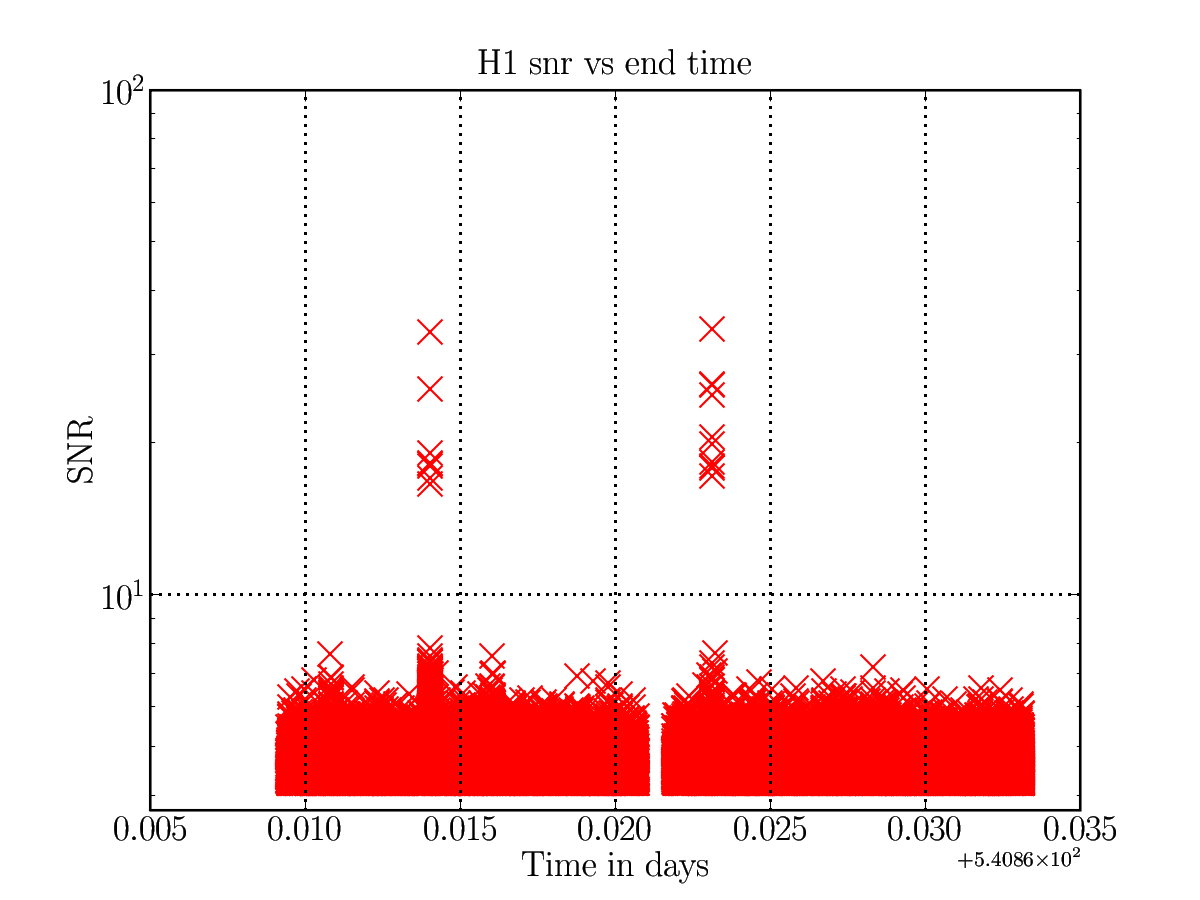
\includegraphics[scale=0.15]{H1_SNR_time.png}
\caption{SNR vs. time in H1}
\label{fig:figure1}
\end{minipage}
\hspace{0.5cm}
\begin{minipage}[b]{0.5\linewidth}
\centering
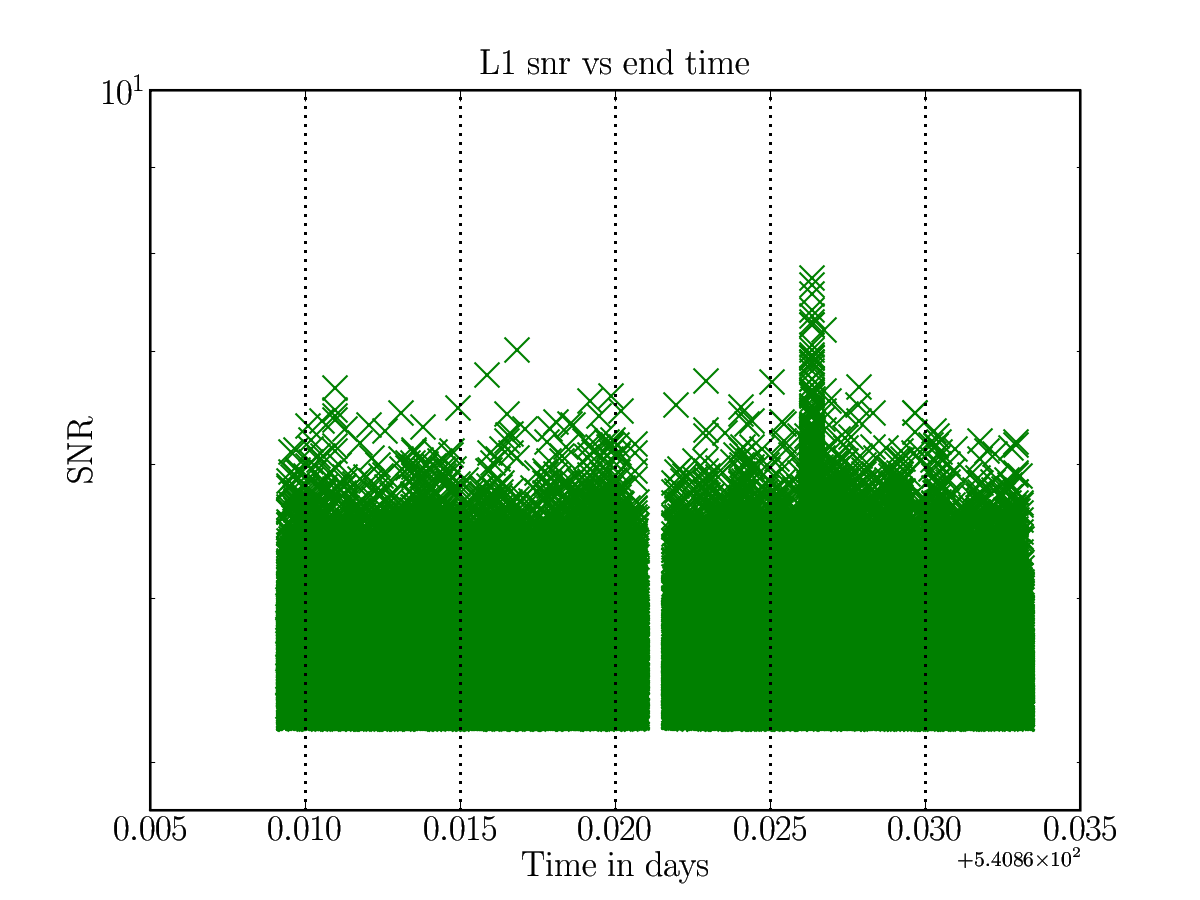
\includegraphics[scale=0.15]{L1_SNR_time.png}
\caption{SNR vs. time in L1}
\label{fig:figure2}
\end{minipage}
\end{figure}

\begin{figure}[ht]
\begin{minipage}[b]{0.5\linewidth}
\centering
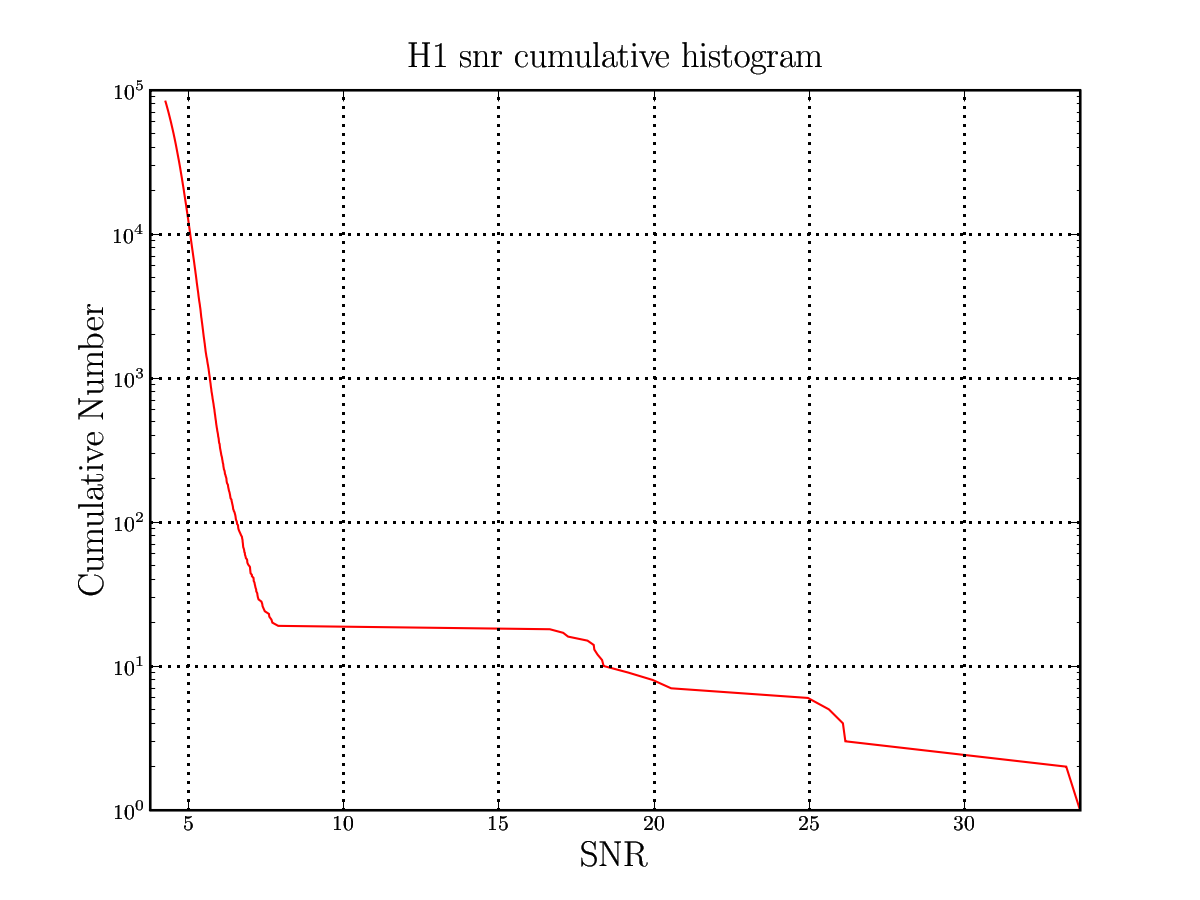
\includegraphics[scale=0.15]{H1_cumno_SNR.png}
\caption{Cummulative number of triggers versus SNR in H1}
\label{fig:figure3}
\end{minipage}
\hspace{0.5cm}
\begin{minipage}[b]{0.5\linewidth}
\centering
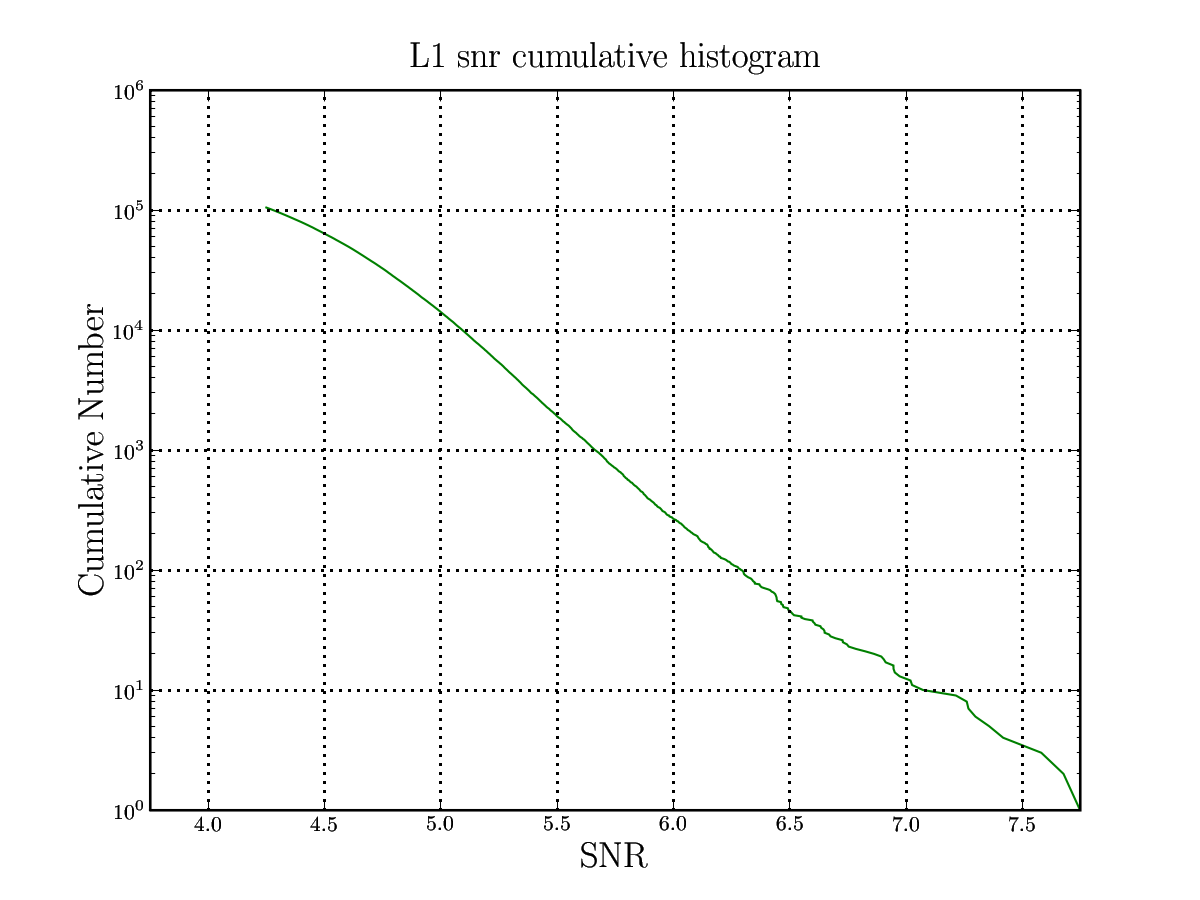
\includegraphics[scale=0.15]{L1_cumno_SNR.png}
\caption{Cummulative number of triggers versus SNR in L1}
\label{fig:figure4}
\end{minipage}
\end{figure}

As seen from the plots above, the data in the H1 detector has a few very loud glitches ($SNR\geq30$,less than 10 glitches) whereas the data in L1 is rather smooth and lacking loud glitches. The glitches in H1 will be subsequently eliminated from the data in the next steps of the analysis. In both Figures ~\ref{fig:figure1} and ~\ref{fig:figure2} the gap inbetween the trigger clusters represents the on-source (the 6 s around the GRB trigger).   

 An SNR threshold cut was applied for the triggers seen in the plots above, that is, triggers are kept only they have SNRs greater than a minimum SNR, set individually for each detector according to the available data for each GRB and that maximizes the sensitivity/computational cost ratio. The threshold SNR was set to 4.25 in the case of H1 and L1 GRB analysis (\cite{grb}). Template masses and trigger times are stored for further investigations. 

Next, coincidence tests are applied on these resulting triggers. The first coincidence test, called Ethinca (detailed in \cite{craig}), searches for triggers with the same masses and trigger times that have to coincide at least in two detectors (in the case of GRB070429B it $is$ only two detectors) and is a powerful noise exclusion tool . The Ethinca (or elliptical thinca) code is a rather new coincidence algorithm for determining if triggers from different detectors are in coincidence. It computes a three dimensional ellipse in the signal space (typically determined by the coordinates coalescence time, $\tau_0$, and $\tau_3$ where $\tau_0$ and $\tau_3$ are two independent functions of component masses that considrebly flatten the parameter metric), with a size determined by the ethinca parameter. If these ellipses overlap, then triggers are considered to be coincident. The degree of coincidence is therefore quantified by the Ethinca parameter, the smaller the Ethinca parameter is, the better a coincidence is confirmed. The threshold Ethinca parameter value above which a coincidence is no longer confirmed was set to 0.8 in the case of the GRB search. Plots of the Ethinca parameter for both H1 and L1 can be seen in Figures ~\ref{fig:figure5} and ~\ref{fig:figure6}; the total number of coincident triggers is listed in the plots'legend with red dots being coincidences from injections and black crosses coincidences from off-source trials.

\begin{figure}[ht]
\begin{minipage}[b]{0.5\linewidth}
\centering
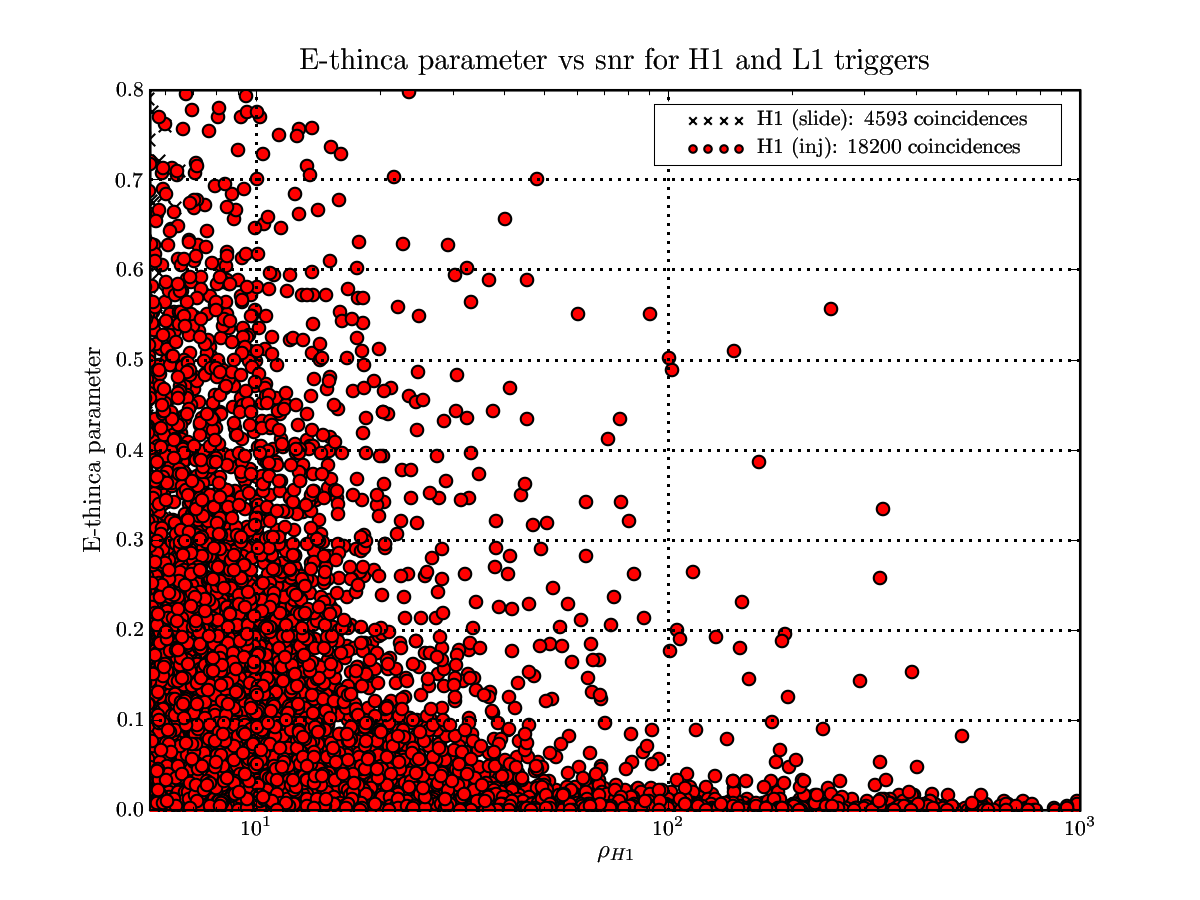
\includegraphics[scale=0.15]{Ethinca_H1.png}
\caption{Ethinca parameter versus SNR in H1 detector}
\label{fig:figure5}
\end{minipage}
\hspace{0.5cm}
\begin{minipage}[b]{0.5\linewidth}
\centering
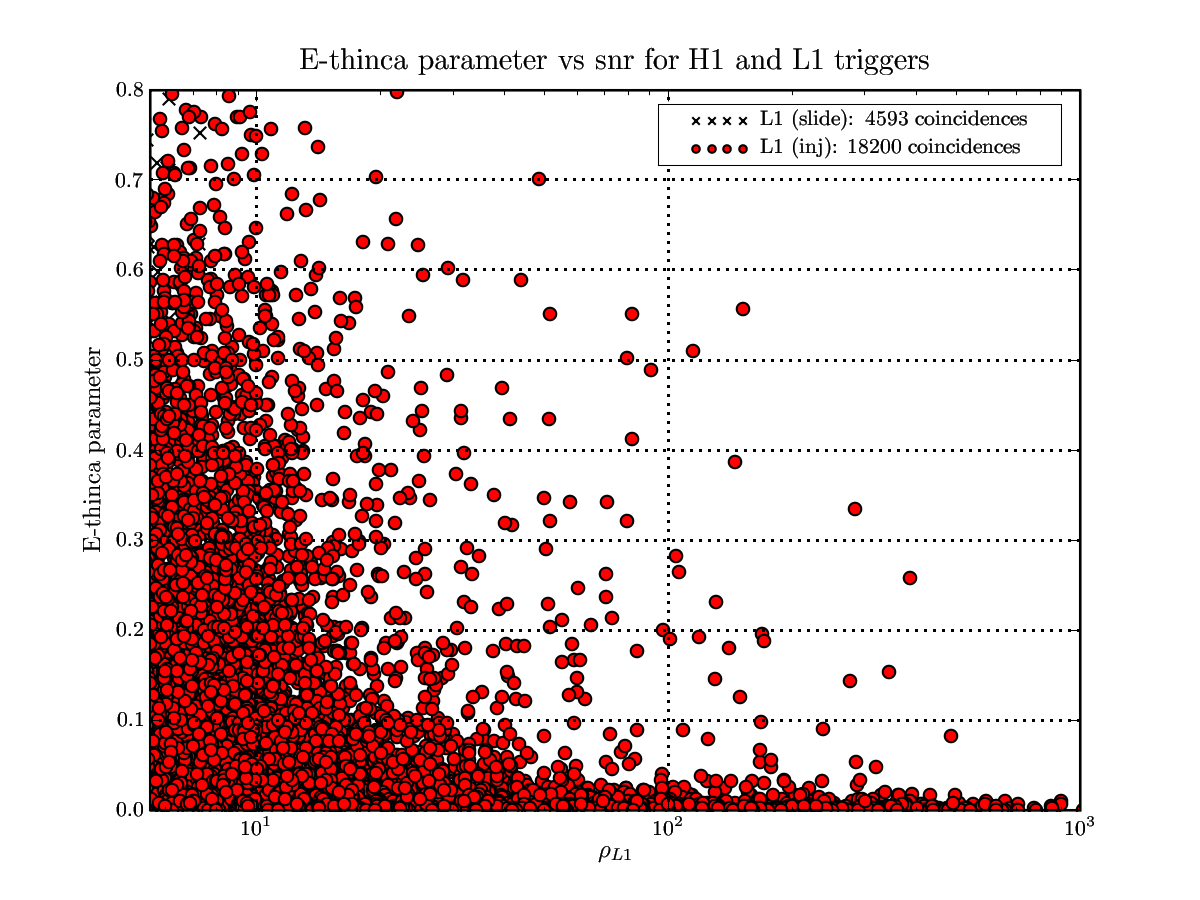
\includegraphics[scale=0.15]{Ethinca_L1.png}
\caption{Ethinca parameter versus SNR in L1 detector}
\label{fig:figure6}
\end{minipage}
\end{figure}

 The triggers that survive the coincidence test are stored and component masses, coalescence phases and effective distances are computed from the templates they were matched against. 

Consistency tests are then applied, such as the $\chi^2$ (\cite{grb,allen,cre}), in order to differentiate between triggers consistent with a possible signal and noise triggers. The $\chi^2$ has been qualitatively described in the Data Analysis section above. Figures ~\ref{fig:figure7} and ~\ref{fig:figure8} show the the distribution of $\chi^2$ versus SNR ($\rho$) for injections (red crosses) and for off-source triggers (blue stars). The colored continuous lines represent lines of constant effective SNR. We observe that the injections (simulated signals) follow a desired evolution in $\chi^2-\rho$ space maintaining a relatively low $\chi^2$ for SNRs of up to 100, whereas the triggers jump in $\chi^2$ values for low values of SNR.

\begin{figure}[ht]
\begin{minipage}[b]{0.5\linewidth}
\centering
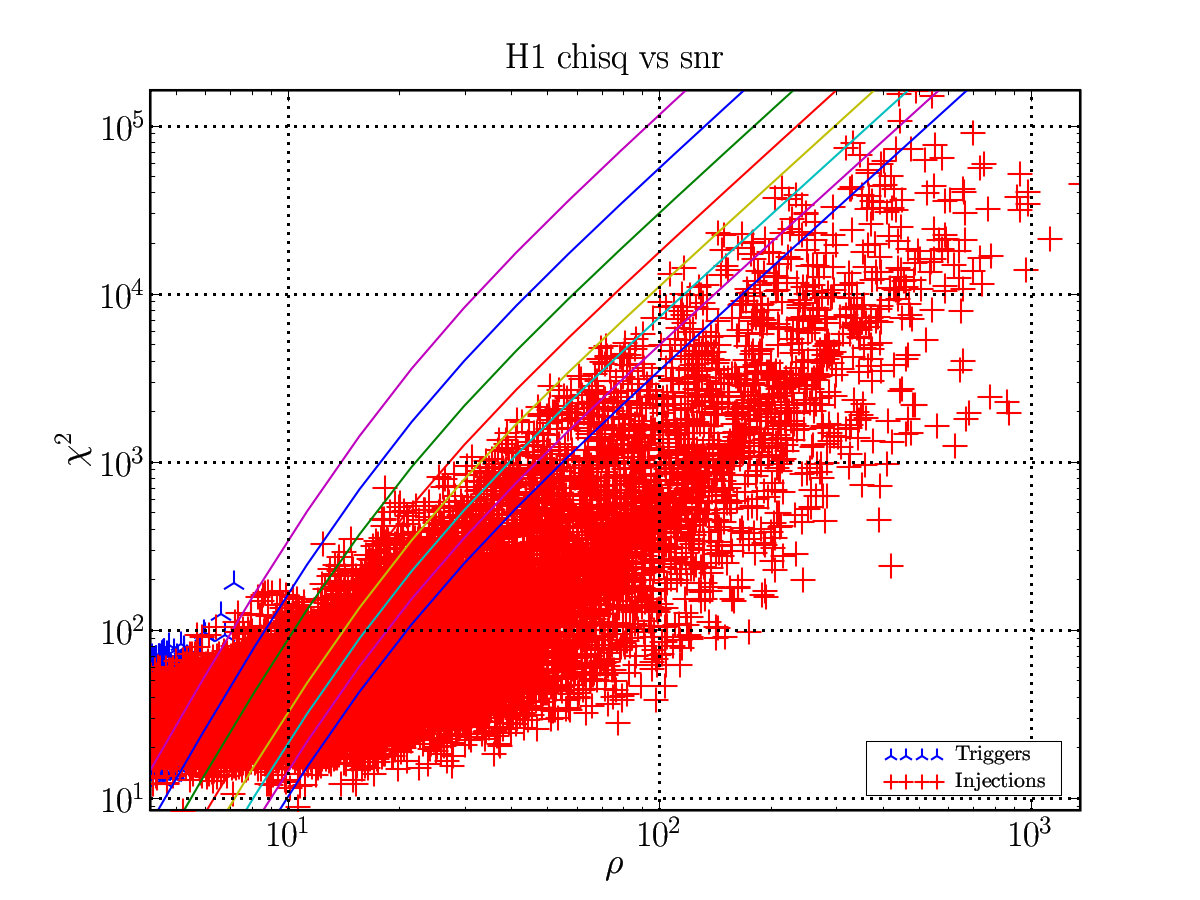
\includegraphics[scale=0.15]{Chisq_H1.png}
\caption{Chi square versus SNR for injections and triggers in H1}
\label{fig:figure7}
\end{minipage}
\hspace{0.5cm}
\begin{minipage}[b]{0.5\linewidth}
\centering
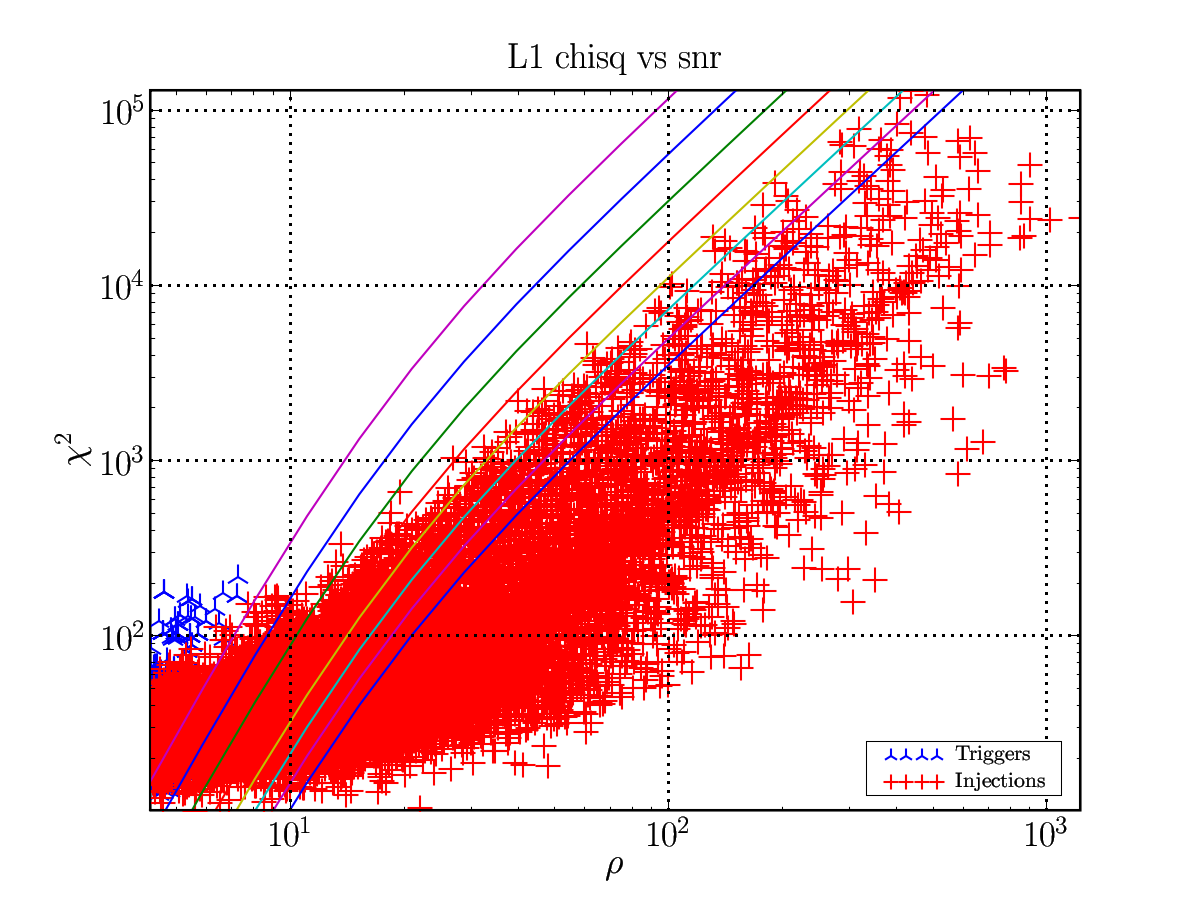
\includegraphics[scale=0.15]{Chisq_L1.png}
\caption{Chi square versus SNR for injections and triggers in L1}
\label{fig:figure8}
\end{minipage}
\end{figure} 

The SNRs and  $\chi^2$ test results from each detector are combined into an effective SNR and the effective SNRs from H1 and L1 are added in quadrature to obtain a cummulative effective SNR (\cite{abbott2006,abbott2007,grb}). The effective SNR has been used as detection statistic in the S3, S4 and S5 science runs (\cite{abbott2007,grb}). It is a combination of the signal to noise ratio and the chi-squared value. For a signal with relatively small SNR and an average value of the chi-squared veto the value of effective snr is equal to the SNR. However, for a signal with a large chi-squared value, the effective $\rho$ is reduced according to equation ~\ref{eqn:roeff}:

\begin{equation}
\rho^2_{{\rm eff}} = \frac{\rho^2}{\sqrt {( \frac {\chi^2}{2p-2})(1+ \frac {\rho^2}{250})}}
\label{eqn:roeff}
\end{equation}

In equation ~\ref{eqn:roeff} $p$ is the number of degrees of freedom in the $\chi^2$ measure, here 16. The denominator 250 is chosen to best separate the background (off-source) from signal (as seen in the Chi squared plots above, the signal, represented by the red injections, sparated from the blue stars, the off-source triggers).

 According to their cummulative effective SNRs, the surviving triggers are gathered in a candidate list which will be partitioned in three mass bins, according to the chirp mass (given by equation ~\ref{eqn:chirpmass} ) recovered for every candidate ($M_c \in [0.86,3.48)$, $[3.48,7.40)$, $[7.40,17.5)$).The cummulative number of candidates versus the effective SNR for the three chirp mass bins is plotted in Figures ~\ref{fig:9} , ~\ref{fig:10} and ~\ref{fig:11}. The subsequent candidates in their corresponding mass bins will be ranked based on a likelihood statistic and detection or upper limits are set according to this statistic.

\begin{figure}[ht]
\begin{minipage}[b]{0.5\linewidth}
\centering
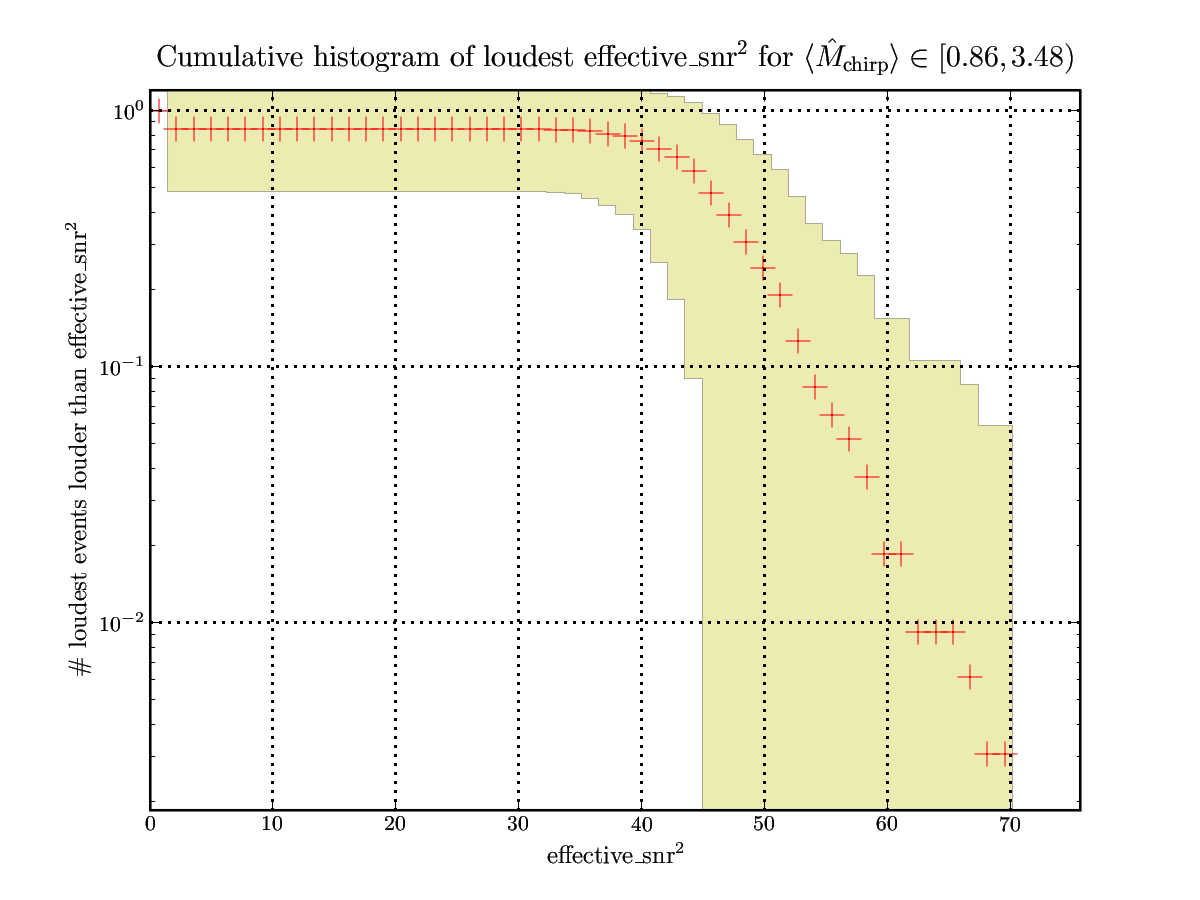
\includegraphics[scale=0.15]{Triggers_Mc1.png}
\caption{Cummulative no. of loudest coincident triggers in low chirp mass bin}
\label{fig:9}
\end{minipage}
\hspace{0.5cm}
\begin{minipage}[b]{0.5\linewidth}
\centering
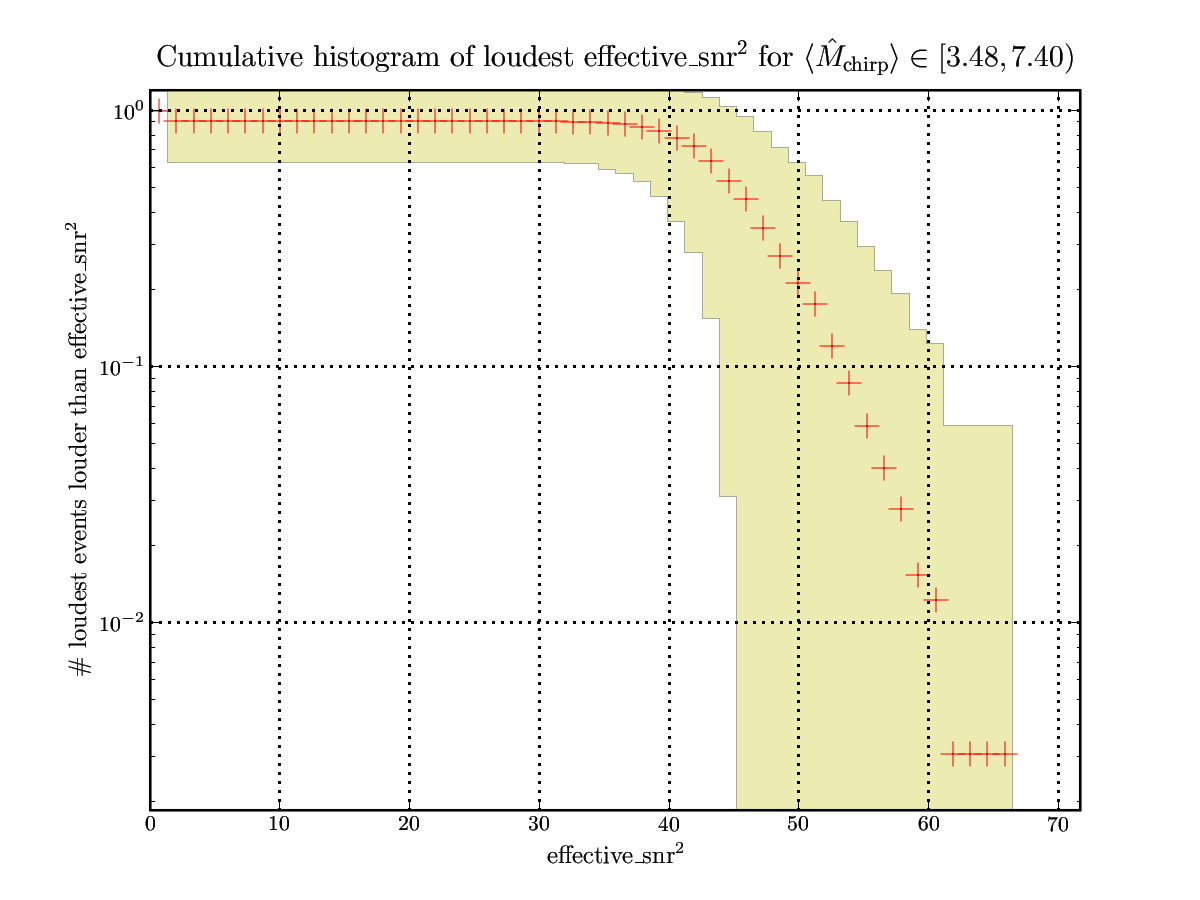
\includegraphics[scale=0.15]{Triggers_Mc2.png}
\caption{Cummulative no. of loudest coincident triggers in medium chirp mass bin}
\label{fig:10}
\end{minipage}
\end{figure}

\begin{figure}[ht]
\centering
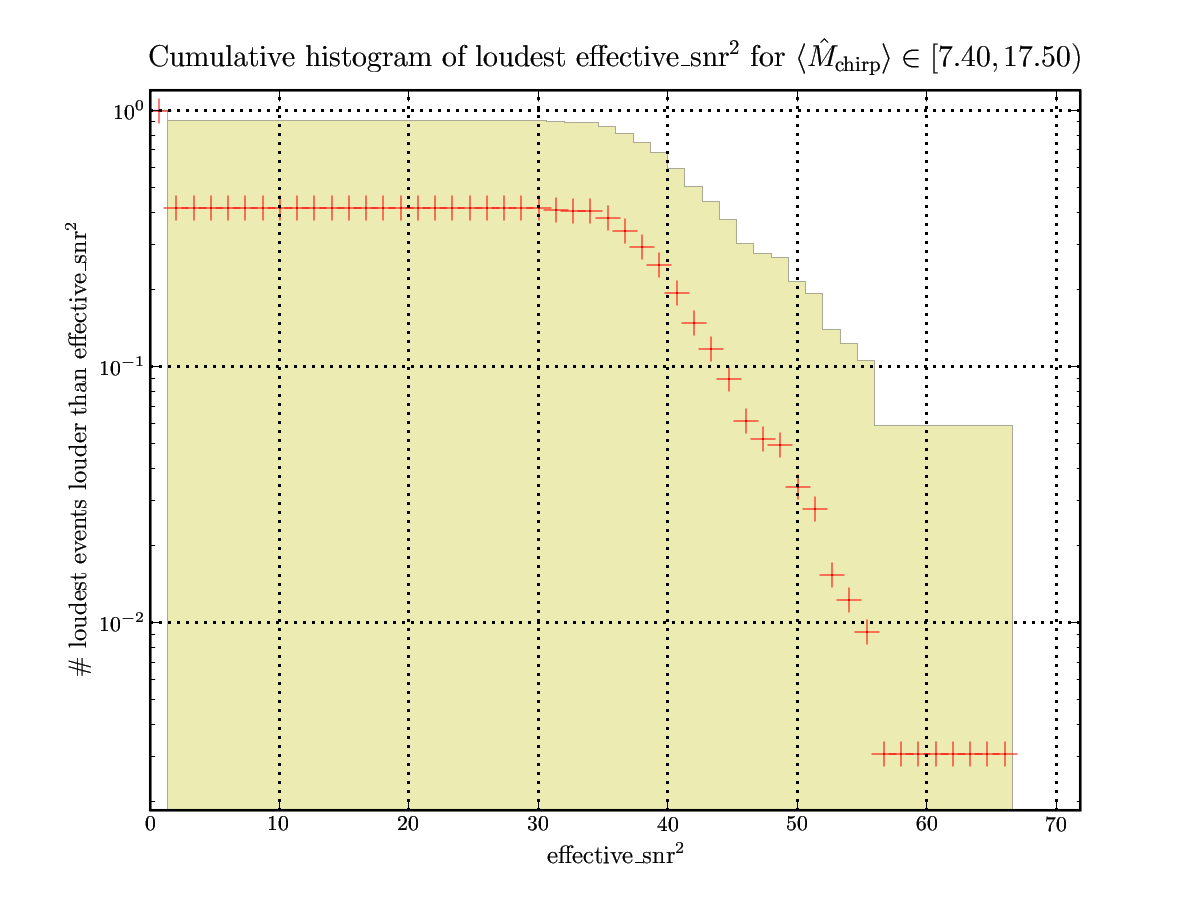
\includegraphics[scale=0.15]{Triggers_Mc3.png}
\caption{Cummulative no. of loudest coincident triggers in high chirp mass bin}
\label{fig:11}
\end{figure}

A very important part of the analysis and post processing of the data is injecting the simulated signals into the data, in the very initial stage of the analysis. Different kinds of waveforms are injected, and the majority of them are found (an injection is considered found if there is a trigger found within 100 ms of the time of the simulation; that trigger being the found injection). Reasons for not finding an injection range from the existence of a very loud detector glitch at the time of the injection, a very poor choice of parameters in the simulation (is is mostly referred to high-spin simulations) and a poor recovery of the parameters (very high $\chi_2$). The missed/found injections plots are shown in Figures ~\ref{fig:figure12} and ~\ref{fig:figure13}. There is a cluster of loud glitches in H1 at around t=0.014 s and again at around t=0.023. A glitchy peak in SNR can be seen in L1 at around t=0.026 s. If we look at the found/missed injections plot on a time-scale we observe that in H1 there are two clusters of missed injections at exactly t=0.014 s and around t=0,023. The same plot for L1 this time shows a cluster of missed injections within 5 ms of t=0.025 s. Hence the conclusion is that most of the missed injections are due to glitches and spin.

\begin{figure}[ht]
\begin{minipage}[b]{0.5\linewidth}
\centering
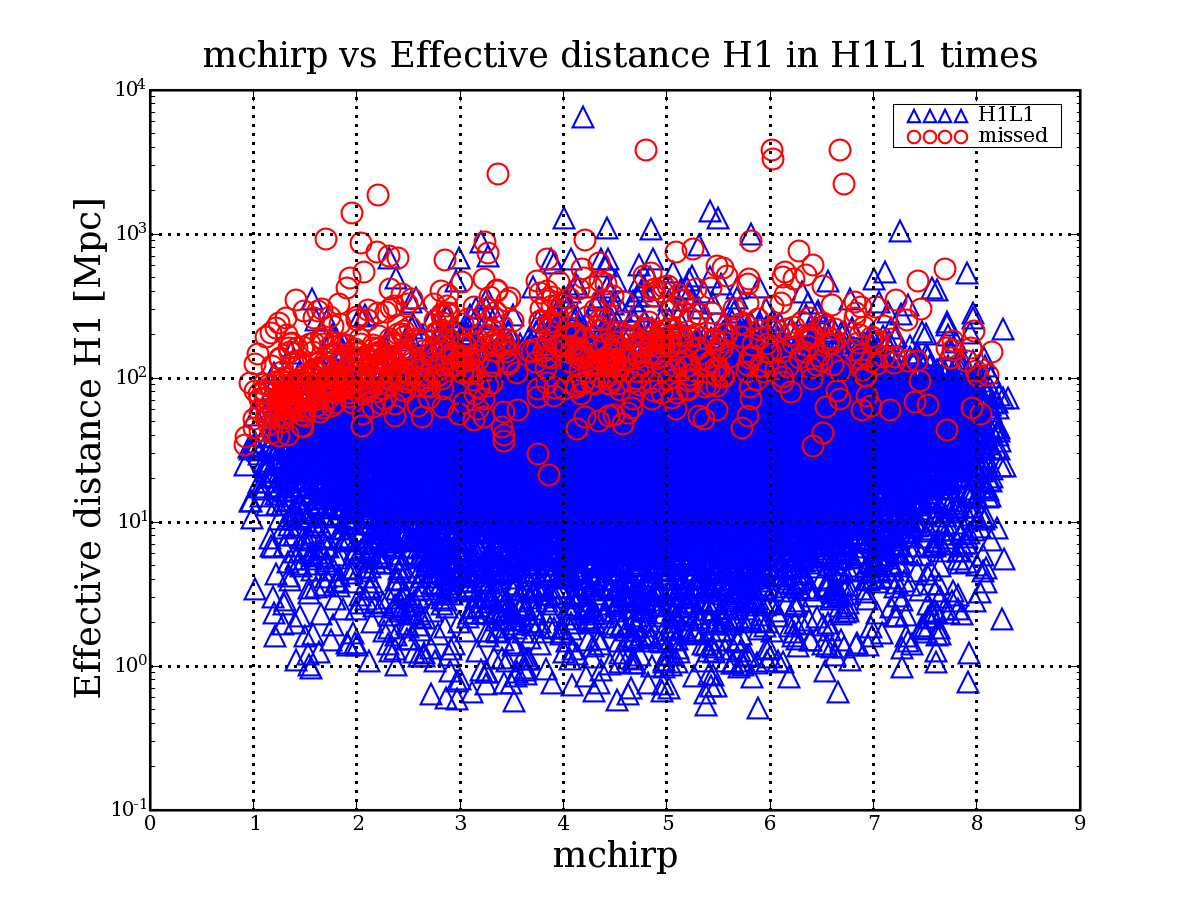
\includegraphics[scale=0.15]{Foundmissed_INJ_H1.png}
\caption{Found/missed injections in H1}
\label{fig:figure12}
\end{minipage}
\hspace{0.5cm}
\begin{minipage}[b]{0.5\linewidth}
\centering
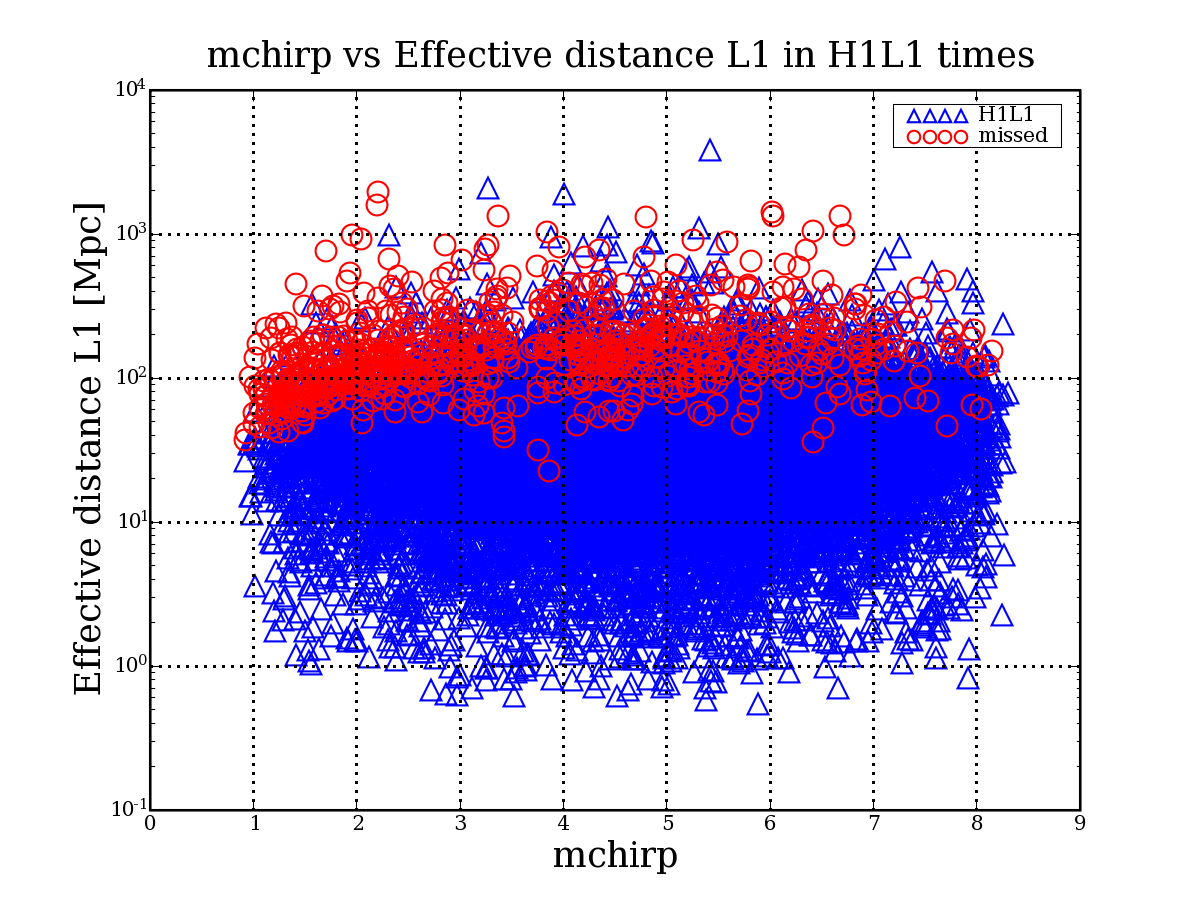
\includegraphics[scale=0.15]{Foundmissed_INJ_L1.png}
\caption{Found/missed injections in L1}
\label{fig:figure13}
\end{minipage}
\end{figure}
 

Consider now the space of chirp masses divided into the three bins, as explained above and in \cite{grb}. Also consider $P(c_i({\bf \theta}) \in \sum|0)$ the probability that a certain $i$ coincident off-source event $c_i=c_i({\bf \theta})$ being a function of a ${\bf \theta}$ parameter vector (combined effective SNR, masses, inclination, polarization etc as scalar components) lies in the semibounded region $\sum$ of the loudest event in each of the chirp mass bins for every of the 300 off-source trials. The region is bounded at the lower end by the loudest event (highest SNR in the chirp mass bin per trial) and at the higher end is open. $P(c_i({\bf \theta}) \in \sum|0)$ is called the false alarm probability, in other words, the probability of assigning GW signal status to a coincident event that is drawn from the set of noise triggers. This probability is a function of effective SNR and should be as low as possible in order to make a positive detection statement. The lowest value we can get in the case of the GRB search is 1/300 since there are 300 off-source trials.

Consider now  $P(c_i({\bf \theta}) \in \sum|h({\bf \alpha}, {\bf \beta}))$ the efficiency of the pipeline of finding GW signals, that is, the efficiency of finding the simulations (injections) from the off-source, in other words the ratio of found over number of injected simulations.  The efficiency will depend on the waveform  $h({\bf \alpha}, {\bf \beta})$ which will in turn depend on two sets of parameters - parameters ${\bf \alpha}$ which are not to be marginalized over and hence are intrinsic to the search (luminosity distance $D$ and companion mass $m_{{\rm comp}}$)  and parameters ${\bf \beta}$ that we will marginalize over with a prior distribution $p({\bf \beta})$ and hence are extrinsic to the detection statement (polarization, inclination, time of coalescence etc). 

Defining now the likelihood as a function of the $\alpha$ parameters as in the following:

\begin{equation}
L({\bf \alpha}, \rho_{{\rm eff}})= \frac {\int P(c_i({\bf \theta}) \in \sum|h({\bf \alpha}, {\bf \beta})) p({\bf \beta}) {\rm d} {\bf \beta}}{P(c_i({\bf \theta}) \in \sum|0)}
\end{equation}

Marginalization over the extrinsic parameters (also called nuisance parameters) has been done with uniform priors in the case of GRB070429B. The likelihood  $L({\bf \alpha}, \rho_{{\rm eff}})$ is hence, after marginalizing over the nuisance parameters, a function of the only two parameters that we haven´t marginalize over and effective SNR:

\begin{equation}
L({\bf \alpha}, \rho_{{\rm eff}}) = L(D, m_{{\rm comp}}, \rho_{{\rm eff}})
\end{equation}

With a prior constant in volume ($D^3=const.$) we can further marginalize the likelihood and obtain a two-variable function, $L=L(m_{{\rm comp}}, \rho_{{\rm eff}})$ and even more, integrate over the template companion mass space to obtain the likelihood as a function of SNR. In terms of a detection statement, one can plot a sum of 3 likelihoods from 3 observed background events versus the respective SNRs and place the loudest event from the foreground (on-source) on this plot, hence comparing where it lies with respect to noise. Such a plot, part of the open box collection of plots, is shown in Figure ~\ref{fig:background} with a slightly different labelling of the axes, basically having sum of marginalized likelihoods $\sum L_n(\rho_{eff})$ on the $y$ axis and effective SNR on the $x$ axis. The dotted line represents the loudest on-source event and as seen from the plot, is perfectly consistent with noise, unfortunately.

 As stated above, the detection statement is based on where the observation likelihoods from the on-source lie with respect to the trigger likelihoods from the background (off-source). The open box plots of GRB070429B show this in the three chosen chirp mass bins: Figure ~\ref{fig:far} plots the false alarm rate $P(c_i({\bf \theta}) \in \sum|0)$  in the $M_{{\rm chirp}}-\rho_{{\rm eff}}$ space and it is visible that the lowest FAR is obtained in the high chirp mass bin, with a value of 0.117, which is by no means a satisfactory value towards a positive detection statement (since the lowest possible FAR is 1/300) and with an effective SNR of about 6.5 which corresponds to a fairly loud off-source noise trigger.  


\begin{figure}[ht]
\begin{minipage}[b]{0.5\linewidth}
\centering
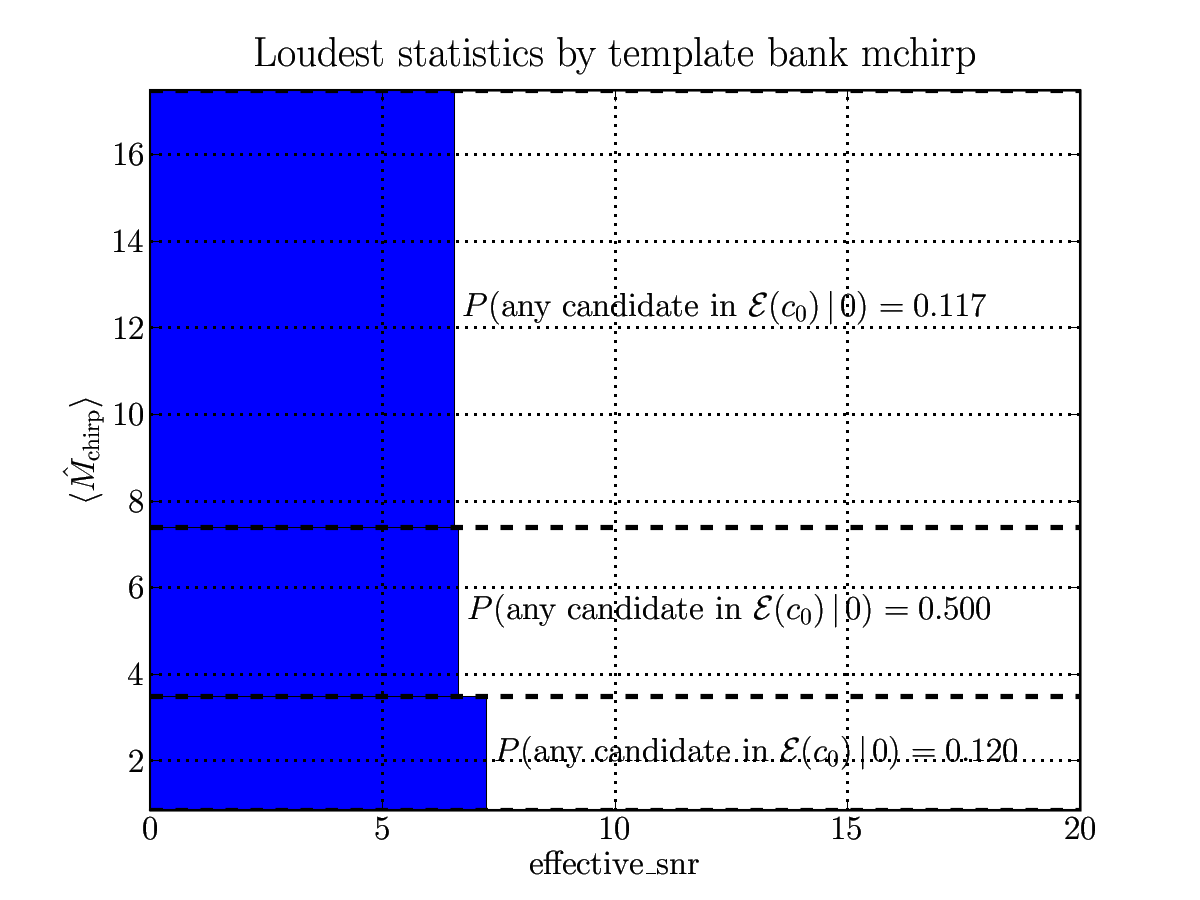
\includegraphics[scale=0.15]{FAR.png}
\caption{False alarm rate probability for the on-source segment of GRB070429B}
\label{fig:far}
\end{minipage}
\hspace{0.5cm}
\begin{minipage}[b]{0.5\linewidth}
\centering
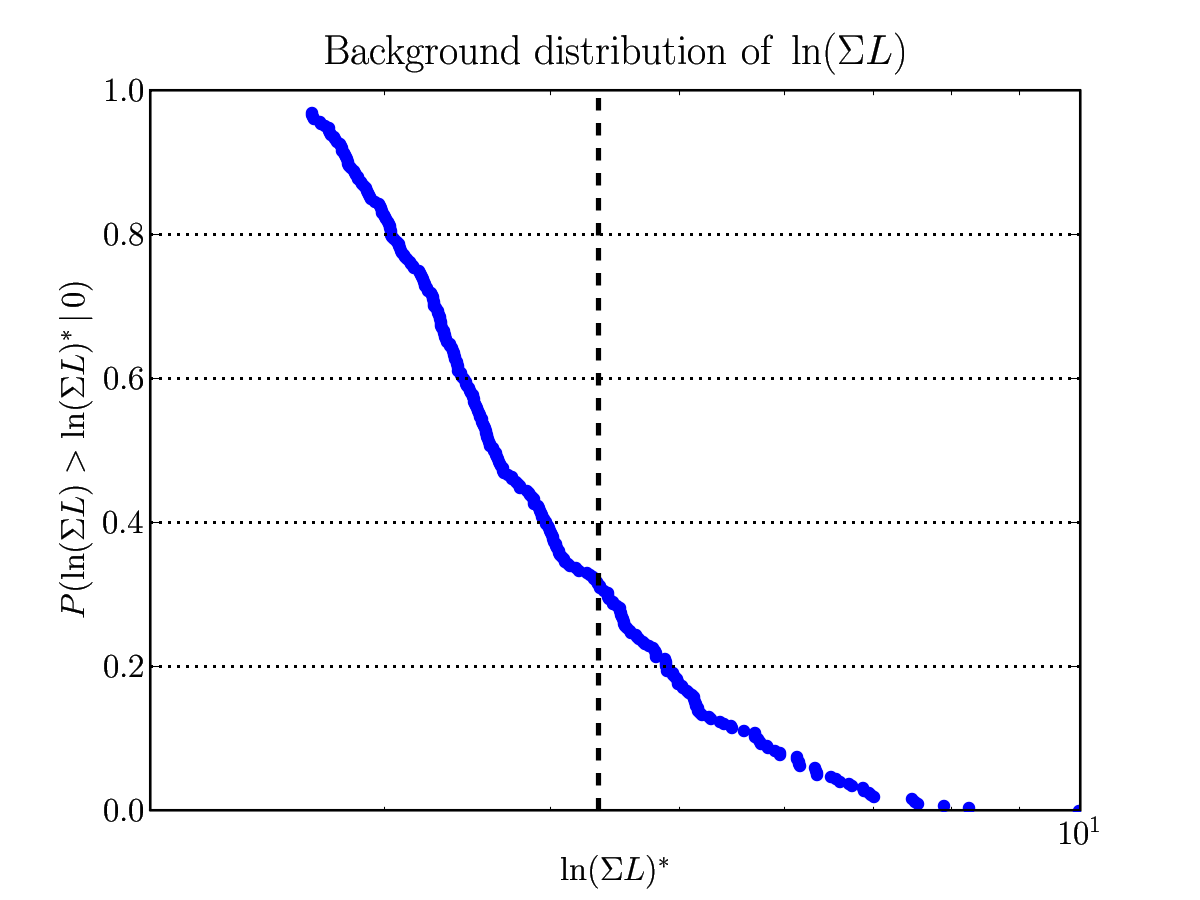
\includegraphics[scale=0.15]{background.png}
\caption{Background events distribution with dotted line the loudest on-source trigger}
\label{fig:background}
\end{minipage}
\end{figure}

As a conclusion to the analysis of GRB070429B, no gravitational waves have been discovered. This statement can be supported by the findings in the on-source segment: the loudest trigger with an SNR of $\sim$6.5 and false alarm rate of 0.117. This trigger´s characteristics are consistent with typical background triggers. The fact that the GRB is thought to be taken place at a luminosity distance of $\sim$4Gpc, far beyond the detectors´ distance range (\cite{abbott2006,abbott2007,grb}), supports the non-detection statement.

\subsection{Timeslides Calculations}

\subsubsection{Introduction}
There is a series of questions that still need to be answered when it comes to estimating the background during a coincident inspiral search for GW when using the timeslides method, in the specific case of searches associated with GRBs. Suppose one performs $S$ timeslides with a slide amount which is much larger than the largest possible coincidence window on a stretch of data of length $T$. One needs to answer these questions before concluding that by doing timeslides one will gain in sensitivity:
\begin{itemize}
\item
What is the desired sensitivity of the search, in other words, what is the range of false alarm rates (FAR) (or probability, FAP) a detection result should be quoted with? This should be answered by using an astrophysical model of the source distribution and not using statistical properties of the GW data.
\item
What is the maximum number of timeslide that one can perform so that one can still gain in senisitivity -- that is, up to what $S^{max}$ can one go so that the FAR (FAP) will still decrease and reach the minimum quoted by answering the above question?
\item
How independent will be the resulting coincidences from doing slides, knowing that the timeslides method does not produce new triggers but rather recycles the existing triggers present in the initial stretch of data and rearranges them to create new coincidences? That is, having a Poisson distributed collecton of single detector triggers, that will be creating coincidences, which triggers will be prone to repeat in coincidences more often than the others, if there is any preference towards such a behavior at all?
\item
How will a loud noise trigger and a glitch affect the statistics by propagating in coincidence and being the loudest event in coincidence?
\item
What is the nominal sensitivity of the search, in other words, what is the maximum false alarm rate (FAR) (or probability, FAP) and its error a detection result should be quoted with, with figures extracted from the statistical properties of the GW data? Is this sufficient, i.e. how does it compare to the one quoted by answering the first question?
\end{itemize}
%

\subsubsection{What is the astrophysically motivated desired sensitivity of the search?}

When are we going to claim we made a detection? The lower estimate of the FAR in order for one to claim a detection is obtained by appying an astrophysical model, i.e. prior, on the distribution of short GRBs in the Local Universe. 

One way of answering this question is by quoting an occurrence rate for short GRBs in the Local Universe (at redshift zero). From \cite{Nakar} we learn that the range for the volume rates for short hard GRBs considered compact binary mergers, at redshift null, can be written as:
%
\begin{equation}
10 ~\leq~ \mathrm{R}_{\mathrm{GRB}=\mathrm{merger}}(z=0) ~\leq~ 10^4 \mathrm{Gpc^{-3}yr^{-1}}
\end{equation}
%

Assuming a maximum range of 40 Mpc for the LIGO I detectors, the volume rate can be expressed as a detector detection rate or true alarm rate:
%
\begin{equation}
7 \times 10^{-4} ~\leq~  \mathrm{R}_{\mathrm{GW},\mathrm{GRB}} ~\leq~  7 \times 10^{-1} \mathrm{yr^{-1}}
\end{equation}
%
or
%
\begin{equation}
\label{rateYEAR}
2 \times 10^{-11} ~\leq~  \mathrm{R}_{\mathrm{GW},\mathrm{GRB}} ~\leq~  2 \times 10^{-8} \mathrm{Hz}
\end{equation}
%

According to (\ref{rateYEAR}), if we did a single search over a one year peried and found a loud candidate, the range of false alarm rates one should associate with it should be $2 \times 10^{-11}$ and $2 \times 10^{-8}$ Hz but if we did a search over a span of roughly 2000s one would want to quote a larger FAR:
%
\begin{equation}
\label{rate2000s}
3 \times 10^{-7} ~\leq~  \mathrm{FAR}_{\mathrm{GRB},2000s} ~\leq~  3 \times 10^{-4} \mathrm{Hz}
\end{equation} 
%
An alternative way of computing the desired FAR is to look at how the GRBs are distributed in volume.
Short hard GRBs are cosmological events but a volume distribution function has not been derived yet. The lack of statistical information concerning a putative volume distribution in the present scientific literature prompted a hands-down look at the available data. The table below contains the distances in Gpc and volumes in $\mathrm{Gpc}^3$ to the Swift short GRBs that have a confidentially associated host galaxy, hence known redshift $z$.

\begin{table}[ht!]
 \begin{tabular}{|l|l|l|l|l|l|l|l|l|l|l|l|l|}
 \hline
 D(Gpc) & 1.108 & 13.8 & 3.14 & 1.46 & 0.509 & 5.24 & 5.85 & 2.53 & 2.05 & 21.8 & 5.84 & 9.1 \\
 \hline
 V($\mathrm{Gpc}^3$) & 3.102 & 502.6 & 35.3 & 6.16 & 0.402 & 98.6 & 121.4 & 22 & 13.68 & 924 & 121.2 & 263.7 \\
 \hline
\end{tabular} 
 \caption{Swift short GRBs with associated host galaxies: distances and astrophysical volumes}
 \label{Table 0}
\end{table}
  
The volume listed in the table is the comoving volume, the volume measure in which number densities of non-evolving objects (transients) locked into Hubble flow are constant with redshift. The comoving volume is approximated by the physical volume for distances of up to 4 Gpc:

\begin{figure}[ht!]
\begin{minipage}[b]{1.0\linewidth}
\centering
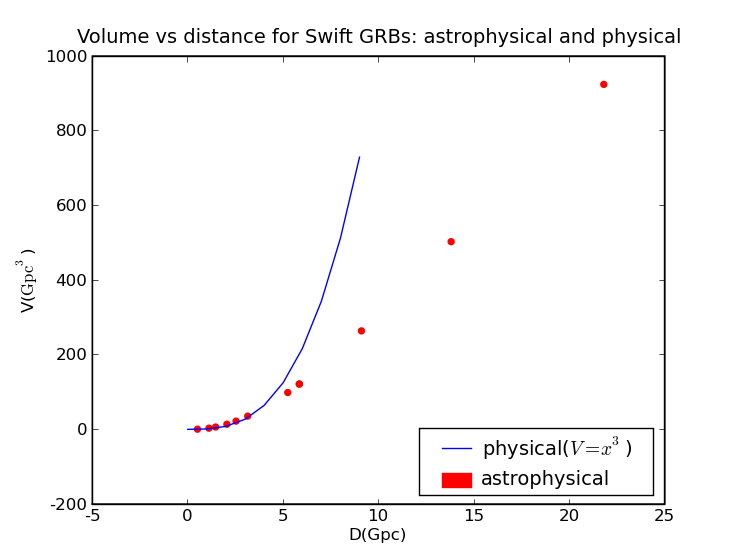
\includegraphics[scale=0.50]{GRBvolume.png}
\caption{Comoving volume (Hubble volume) compared to physical volume for the Swift GRBs with known hosts and redshifts. The red dots represent the GRBs.}
\label{fig:figure1}
\end{minipage}
\end{figure}

Assuming a constant number density for short GRBs within a physical spherical volume with a radius of 4 Gpc and assuming an optimistic average LIGO/Virgo detector range of 40 Mpc and maximum angualr sensitivity within this volume, one can estimate the maximum FAP we should claim for a possible detection statement for a GRB search:

\begin{equation}
\mathrm{FAP}_{max} = \frac{dN_\mathrm{observable}(\mathrm{V_{IFO}}=64 \times 10^{-6} \mathrm{Gpc}^3)}{dN(\mathrm{V_{uniform}}= 64 \mathrm{Gpc}^3)} \approx 10^{-6}
\end{equation}
 
%\section{Maximum number of slides, statistical independence of slides and maximum FAR/P}

\subsubsection{Time only coincidences}

One assumes that the single-detector triggers are Poisson distributed with a constant occurrence rate that varies from one detector to another and from time to time within the same detector (due to excessively noisy or glitchy times, detector maintenance, bad weather, etc). The Poisson approximation is applied for a GRB search that spans a time of around 2000s.By inspecting the first inspiral files one could get the total number of single detector triggers $N_{i}^1$ and $N_{i}^2$ and the trigger rates $R_{i}^1$ and $R_{i}^2$ knowing that the total analysis time is $T$ and that we use the three chirp mass bins. Suppose we analyze data from two detectors, 1 and 2:

\begin{equation}
\label{rats}
R_{i}^1 = \frac{N_{i}^1}{T}, R_{i}^2 = \frac{N_{i}^2}{T}
\end{equation}

where $i$ represents the index for each chirp mass bin (with 0.86,3.48,7.40,17.50 boundaries) and $L,V$ the detector indeces.

The probabilities of having at least one trigger in a coincidence window $\delta$t given the single detector trigger rates $(R_{i}^1,2$ will be:
%
\begin{equation}
\label{pei}
\mathrm{p_i} = \mathrm{p}(R_{i}^1) = 1- \mathrm{e}^{-R_{i}^1 \delta t}
\end{equation}
%
\begin{equation}
\label{qui}
\mathrm{q_i} = \mathrm{q}(R_{i}^2) = 1- \mathrm{e}^{-R_{i}^2 \delta t}
\end{equation}
%
this by choosing a fixed time coincidence window $\delta$t. According to \cite{Was1}, the average number of coincidences will be:

\begin{equation}
\label{farski}
\mathrm{FAR_i} = \frac{n\mathrm{p_iq_i}}{T} = \frac{1}{\delta t} (\mathrm{p_i} \times \mathrm{q_i})
\end{equation}
%
where $n$ is the total number of coincidence windows $n=T/ \delta t$. The variance will be, knowing that $S$ is the total number of timeslides:
%
\begin{equation}
\sigma_i = \sqrt{\mathrm{Var}_i} = \sqrt{\frac{n\mathrm{p_iq_i}}{T^2} \times \frac{1+\mathrm{p_iq_i}-(\mathrm{p_i+q_i})+S(\mathrm{p_i+q_i-2p_iq_i})}{S}}
\label{sigmatime}
\end{equation} 

\subsubsection{Time and mass coincidences in the offsource}

\paragraph{Time-mass coincidence window}
We have written the resulting FAR and its error for the case in which we apply a one dimensional time-only coincidence window. In the standard inspiral CBC analysis three dimensional coincidence elliptical windows are used to find coincidences. Let's consider a rectangular coincidence window for ease of calculation and use notations and numerical results from \cite{japan} and $\delta t$ from the above section:

\begin{eqnarray}
x(\eta, M, d/c, \rho_0) &=& \Delta_w t_c(d/c, \rho_0) \times \Delta_w \tau_0(\eta, M, \rho_0) \times \Delta_w \tau_3(\eta, M, \rho_0) \nonumber\\
                        &\approx& \frac{2a_{\tau_0}a_{\tau_3}}{\rho^2_0} \delta t \nonumber\\
                        &\approx& \frac{4}{\rho^2_0} \delta t ~\mathrm{(s)} 
\end{eqnarray}
%
where $t_c$ is the coalescence time, $\tau_0$ and $\tau_3$ are two functions of total mass $M$ and $\eta$, fraction of reduced mass and total mass, that maximize the signal-to-noise ratio recovered from filtering with a certain template, $d/c$ is the light travel time between the two considered detectrors, $a_{\tau_0}$ and $a_{\tau_3}$ are two constants estimated in \cite{japan} and $\rho_0$ is the signal-to-noise ratio threshold. 

Mass coincidences ($\tau_0$, $\tau_3$) introduce a dimensionless factor $\epsilon(\eta, M, \rho_0) \approx \epsilon(\rho_0) \approx 4/\rho_0^2$ of order 0.16 at threshold signal-to-noise ratio $\rho_0=5$. Grossly approximating the factor as constant across each chirp mass bin, a one dimensional time-only coincidence window $\delta t$ becomes a two-dimensional mass-time coincidence window denoted by $x_i = \epsilon \times \delta t$ in each chirp mass bin $i$ of order 
%
\begin{equation}
x_i = \epsilon \times \delta t \sim 0.1 \times 25 ~\mathrm{ms} \approx 2 \times 10^{-3} ~\mathrm{s}
\end{equation}

Any two events (triggers) from detectors 1 and 2 separated by 
%
\begin{equation}
|\Delta_{12} t_c| \leq |\Delta_w t_c|, |\Delta_{12} \tau_0| \leq |\Delta_w \tau_0|, |\Delta_{12} \tau_3| \leq |\Delta_w \tau_3|
\end{equation}
%
are considered coincident. 


\paragraph{False Alarm Rate and its error}
Replacing equations (\ref{pei}) and (\ref{qui}) in (\ref{farski}) and making the appropriate approximations in the exponential expressions, knowing that the exponents are $\ll 1$:

\begin{equation}
p_i = p(R_{i}^1) = 1- \mathrm{e}^{-R_{i}^1 x_i} \approx R_{i}^1 x_i
\end{equation}
\begin{equation}
q_i = q(R_{i}^2) = 1- \mathrm{e}^{-R_{i}^2 x_i} \approx R_{i}^2 x_i
\end{equation}

we can get an expression for the FAR:

\begin{eqnarray}
\label{faar}
\mathrm{FAR_i} &=& \frac{np_iq_i}{T} \nonumber\\
               &=& \frac{(1- \mathrm{e}^{-R_{i}^1 \epsilon \delta t})(1- \mathrm{e}^{-R_{i}^2 \epsilon \delta t})}{\epsilon \delta t} \nonumber\\
               &=& \frac{(1- \mathrm{e}^{-R_{i}^1 x_i})(1- \mathrm{e}^{-R_{i}^2 x_i})}{x_i} \nonumber\\
               &=& x_iR_{i}^1 R_{i}^2                
\end{eqnarray}

In the case of an inspiral GRB search one can estimate both the rates $R_{i}^{1,2}$ and the mass-time coincidence window $x_i$, hence get an estimate of the FAR, by making a series of assumptions: the coincidence window is constant across each of the three chirp mass bins and does depend only on the threshold SNR, $\rho_0$, (chosen to be constant for the whole search); the rates depend on the threshold SNR and may be approximated as constant across the search when using a constant threshold and apply proper data quality cuts. They can be regarded as simply the total number of single detector triggers divided by analysis time, as in equation (\ref{rats}). For GRB090809B we have the following numbers of first stage (of the pipeline) single detector triggers and rates, listed in Tables \ref{triggers} and \ref{rates}. Note that the detectors are 1=L and 2=V and the division in chirp masses is expressed by the indeces.

\begin{table}[ht]
 \begin{tabular}{|l|l|l|l|l|l|}
 \hline
 \hline
 $N_{1}^L$ & $N_{2}^L$ & $N_{3}^L$ & $N_{1}^V$ & $N_{2}^V$ & $N_{3}^V$ \\
 \hline
 86310 & 9435 & 1423 & 267503 & 19673 & 1494 \\
 \hline
 \hline
 \end{tabular} 
 \caption{GRB090809B: first inspiral trigger counts for L and V detectors for the three chirp mass bins}
 \label{triggers}
\end{table}

\begin{table}[ht]
 \begin{tabular}{|l|l|l|l|l|l|}
 \hline
 \hline
 $R_{1}^L$ & $R_{2}^L$ & $R_{3}^L$ & $R_{1}^V$ & $R_{2}^V$ & $R_{3}^V$ \\
 \hline
 39.41 & 4.31 & 0.68 & 122.15 & 8.98 & 0.68 \\
 \hline 
 \hline
 \end{tabular} 
 \caption{GRB090809B: trigger rates in units of Hz}
 \label{rates}
\end{table}


The variance can be easily derived from equation (\ref{sigmatime}) assuming that $p_i \ll 1$ and $q_i \ll 1$. 

\begin{eqnarray}
\sigma_i = \sqrt{\mathrm{Var_i}} &\approx& \sqrt{\frac{np_iq_i}{\mathrm{T}^2}(\frac{1}{S} + p_i + q_i)} \nonumber\\ 
                                 &=& \sqrt{\frac{x_iR_{i}^1 R_{i}^2}{\mathrm{T}}[ \frac{1}{S} + (R_{i}^1 + R_{i}^2) x_i ]}
\label{far_variance}
\end{eqnarray}

The number of timeslides at which the Poisson error terms $x_i(R_{i}^1 + R_{i}^2)$ equalize the error from doing timeslides, $1/S$, will be improperly called the maximum number of timeslides, $S^{\mathrm{max}}$. It is improperly called maximum since one may choose to do as many timeslides as one wants and there is no physical limit for $S$ simply imposed by the Poisson counting errors. It is just that by increasing the number of timeslides beyond $S^{\mathrm{max}}$ there is very limited gain in sensitivity. Hence, $S^{\mathrm{max}}$ is given by:

\begin{equation}
S^{\mathrm{max}}_i = \frac{1}{x_i(R_{i}^1 + R_{i}^2)}
\label{timeslidesmax}
\end{equation}

In the case of our example GRB, we will \emph{estimate} the magnitude of the coincidence window $x$ in each chirp mass bin by using the single detector rates from Table \ref{rates} and equation (\ref{faar}). The false alarm rates are the number of backgound coincidences divided by the analysis time $T$. This estimation is done for the zerolag and the timeslides (160 timeslides) methods of background analysis and are tabled in Table \ref{xes}, together with the corresponding FAR's.

\begin{table}[ht!]
 \begin{tabular}{|l|l|l|l|l|l|l|l|l|}
 \hline
 \hline
 $x_1$ & $x_2$ & $x_3$ & $\mathrm{FAR}_1$ & $\mathrm{FAR}_2$ & $\mathrm{FAR}_3$ & $\sigma_1$ & $\sigma_2$ & $\sigma_3$ \\
 \hline
 0.00009 & 0.0046 & 0.0346 & 0.435 & 0.179 & 0.016 & 0.0026 & 0.0026 & 0.0007 \\
 \hline
 0.00010 & 0.0041 & 0.0389 & 0.468 & 0.158 & 0.018 & 0.0025 & 0.0022 & 0.0007 \\
 \hline
 \hline
 \end{tabular} 
 \caption{GRB090809B: coincidence windows $x_i$ (s), FAR's and their errors (Hz) obtained using data from the zerolag (S=0, first line) and timeslides (S=160, second line)}
 \label{xes}
\end{table}
 
$S^{\mathrm{max}}$ is decisevely larger for the low chirp mass bin, at about $\sim$70 slides, whreas for the other two chirp mass bins it's not more than $\sim$20 slides.

\paragraph{Equal trigger rates} 
Let's suppose both detectors have the same trigger rate $R^1_i=R^2_i=R$ within the same chirp mass bin $i$ and we consider working in only one of the chirp mass bins, say the low mass one. One can express the false alarm rate in the considered chirp mass bin as $\langle \mathrm{FAR} \rangle= \mathrm{FAR}(1 \pm f)=xR^2(1 \pm f)$ for a fixed (by the analysis) coincidence window $x$ and with $f$ given by the following:

\begin{equation}
f(R, S) = \frac{1}{\sqrt{T}} \sqrt{\frac{2}{R} + \frac{1}{xR^2S}}
\label{fequal}
\end{equation}

By \emph{fixing} the number of timeslides at maximum $S=S^{\mathrm{max}}=1/2xR$ we have:

\begin{equation}
f(R, S=S^{\mathrm{max}}) = \frac{2}{\sqrt{RT}}
\end{equation}

Considering that $f(R)$ should be no more than 0.05 for a 95$\%$ exact result of the false alarm rate, one can extract a desired rate of triggers function of the total time of analysis:

\begin{equation}
\label{1600rate}
R \approx \frac{1600}{T} \mathrm{Hz}
\end{equation}

\begin{equation}
\mathrm{FAR} \approx \frac{2.6 \times 10^4 \times x}{T^2} \mathrm{Hz}
\end{equation}

In other words this would yield a 5$\%$ error of the FAR at maximum number of timeslides if one has roughly 1600 single detector triggers counted in the analysis time $T$.

Since we would ideally want a FAR of about $10^{-5}$ and knowing that for a 5$\%$ FAR error the single detector trigger rate at threshold SNR is given by (\ref{1600rate}), one gets the desired width of the coincidence window for such a FAR:

\begin{equation}
x \approx 4T^2 \times 10^{-11} \mathrm{s}
\end{equation}

For a standard GRB search of about 2000s the coincidence window should be of $\approx 2 \times 10^{-4}$ s and the maximum number of timeslides $S^{\mathrm{max}} \approx 10^6/3$. In conclusion one can get close to a FAR of $10^{-5}$ and a $\sigma$ of $5 \times 10^{-7}$ if the single detector trigger rates approach 1 Hz and 300,000 timeslides are performed with an analysis time of 2000s per slide.

Conversely, by considering a variable number of slides $S$, an equal single detector trigger rate of R=0.32 Hz would yield a FAR=$\mathrm{10}^{-5}$ and and a $\sigma \approx \mathrm{10}^{-6}$ for 5000 timeslides, as seen in Figure~\ref{figure2}.

\begin{figure}[ht!]
\label{figure2}
\centering
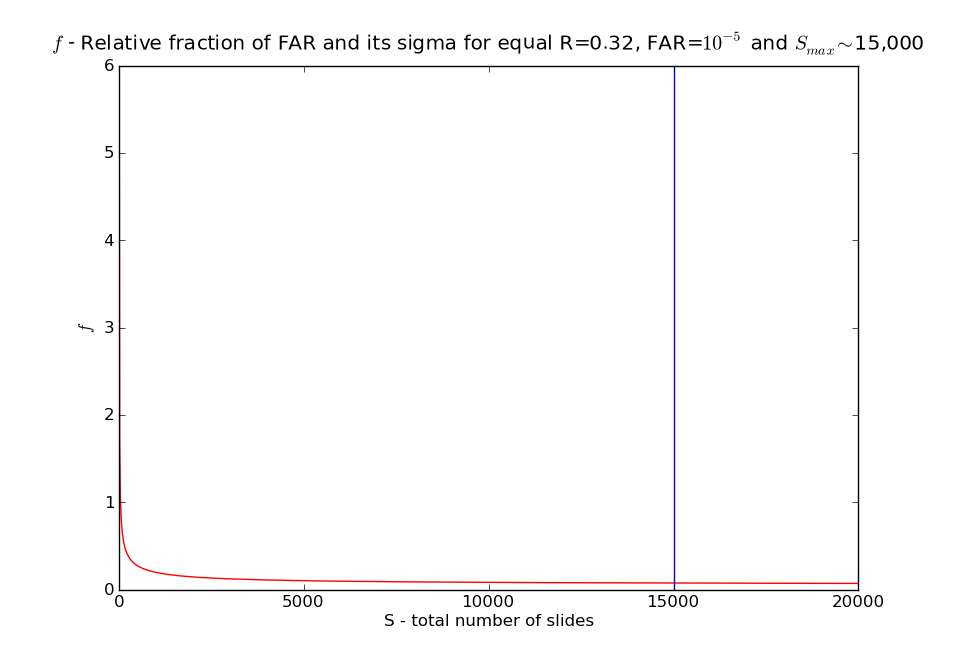
\includegraphics[scale=0.45]{R=032equal_rates.png}
\caption{Fraction $f$ versus number of slides $S$ with $f$(5,000 slides)=0.1, $f$(10,000 slides)=0.08 and $f$(15,000 slides)$\approx f$(20,000 slides)=0.07}
\end{figure}

An analysis time of T=2000s and a trigger rate R=0.32Hz would mean accepting on average about N=650 triggers per detector. This can be easily achieved by applying a higher SNR threshold

\paragraph{Unequal trigger rates}
Consider now that the single detector trigger rates are very different: suppose we take e.g. $R^1 \ll R^2$ hence one can write $f$ as:

\begin{equation}
f(R^1 \ll R^2, S) = \sqrt{\frac{1}{T R^1}} \sqrt{1 + \frac{1}{xSR^2}}
\end{equation}

\begin{equation}
\label{unequalrates}
f(R^1 \ll R^2, S=S^{\mathrm{max}}) \approx \sqrt{\frac{2}{TR^1}}
\end{equation}

Employing the same kind of reasoning as in the above paragraph, we would want to \emph{fix} the number of timeslides at $S=S^{\mathrm{max}}$ and work with a $\mathrm{FAR}=10^{-5}$ with a fractional error of $f=0.05$. From equation (\ref{unequalrates}) one can write down the rate and the false alarm rate:

\begin{equation}
R^1 \approx \frac{800}{T} ~\mathrm{Hz}
\end{equation}
%
\begin{equation}
\mathrm{FAR} \approx \frac{800R^2x}{T} \sim 10^{-5}
\end{equation} 

For an analysis time of 2000s and a trigger rate $R^2$ of order 100 Hz one may be able to reaqch a FAR of $10^{-5}$ if and only if the coincidence window is of order $10^{-4}$ s or smaller.

For a practical example, seen in Figure \ref{figure3} $R^1=0.32$ Hz and $R^2=100$ Hz. In such a case the FAR$\approx 10^{-2}$ Hz and $S^{\mathrm{max}} \approx 100$ as seen from Figure \ref{figure3}. 

\begin{figure}[ht!]
\centering
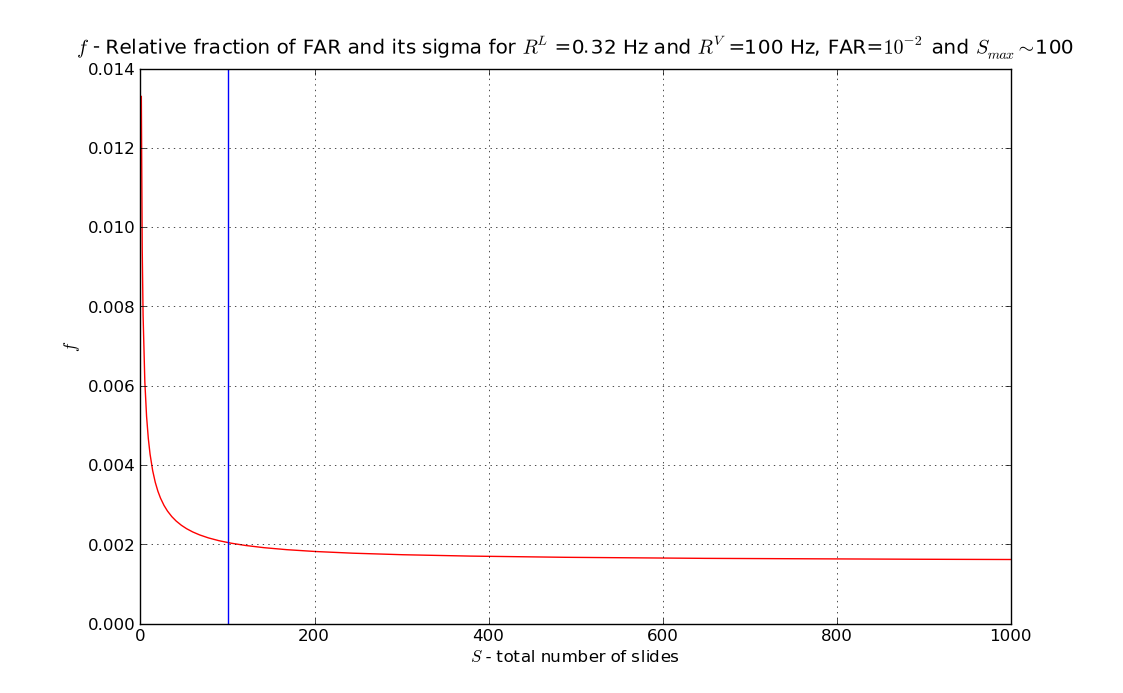
\includegraphics[scale=0.45]{R=032R=100.png}
\caption{Fraction $f$ versus number of slides $S$ with f(100 slides) $\approx$ 0.002 and f(1000 slides) $\approx$ 0.0016}
\label{figure3}
\end{figure}

\paragraph{Repeating triggers and trigger occurrence rates} The same single detector triggers may participate in numerous coincidences when doing timeslides, since the timeslides method of "extending" the background doesn't produce new triggers but rather reuses the same triggers within the analysis time $T$ to create new coincidences at every slide step. Whichever triggers are more prone to repeat in coincidences is not yet known and remains to be further investigated into, but we can create plots that help us understand if the number of times a trigger repeats is a function of any parameter such as chirp mass or SNR, etc. Figure \ref{occurrencefigures} shows such a plot for the example GRB, GRB090809B: number of repeating triggers versus chirp mass.  

\begin{figure}[ht!]
\begin{minipage}[b]{0.7\linewidth}
\centering
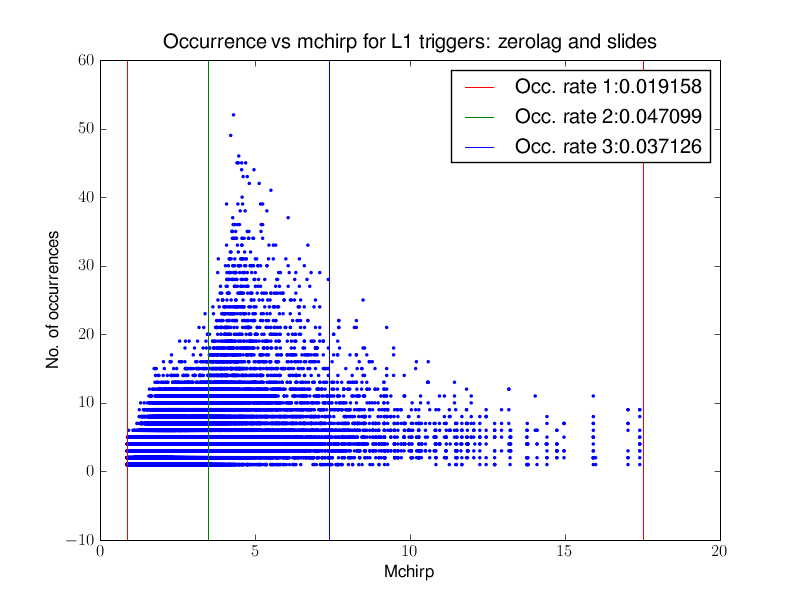
\includegraphics[scale=0.55]{L1_unclustered.png}
%\caption{GRB090809B: number of trigger occurrences of L triggers before trial clustering}
%\label{fig:figure2}
\end{minipage}
%\begin{minipage}[b]{0.4\linewidth}
%\centering
%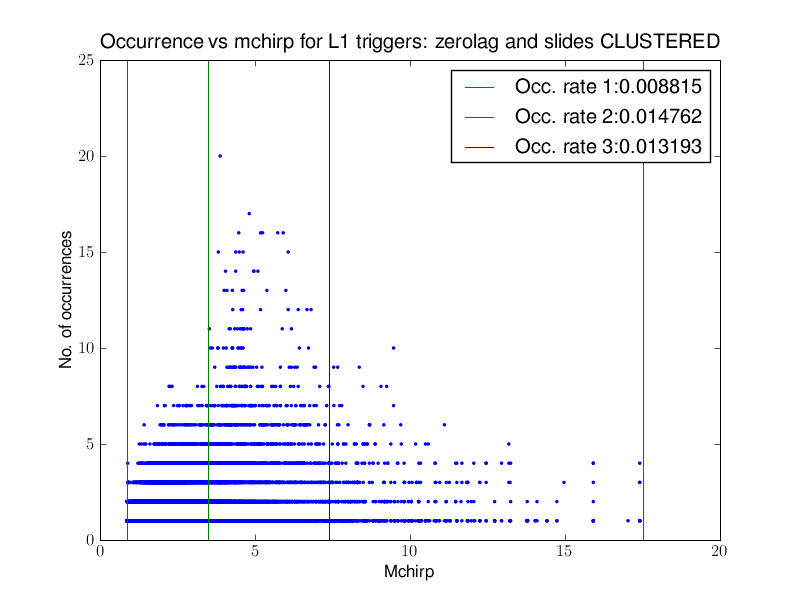
\includegraphics[scale=0.45]{L1_clustered.png}
%\caption{GRB090809B: number of occurrences of L triggers after trial clustering}
%\label{fig:figure3}
%\end{minipage}
%\end{figure}
%\begin{figure}[ht!]
\begin{minipage}[b]{0.7\linewidth}
\centering
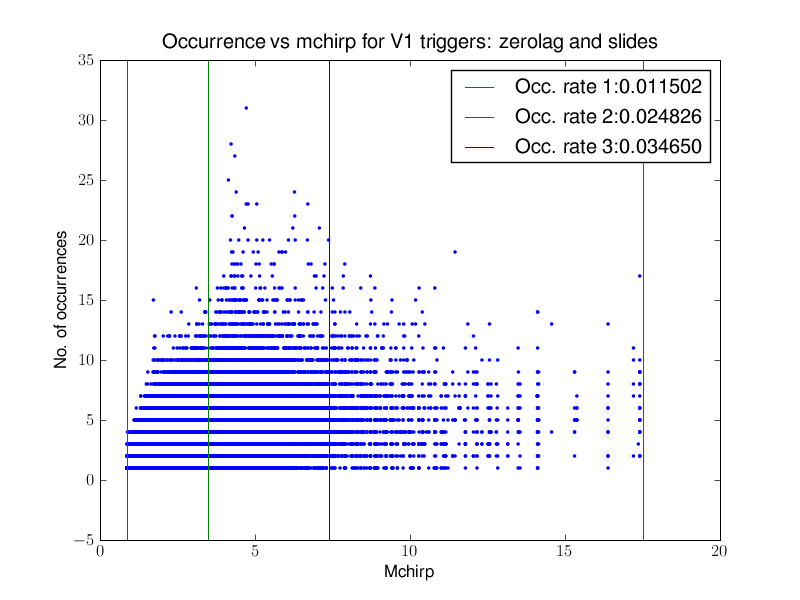
\includegraphics[scale=0.55]{V1_unclustered.png}
%\caption{GRB090809B: number of occurrences of V triggers before trial clustering}
%\label{fig:figure3}
\end{minipage}
%\begin{minipage}[b]{0.4\linewidth}
%\centering
%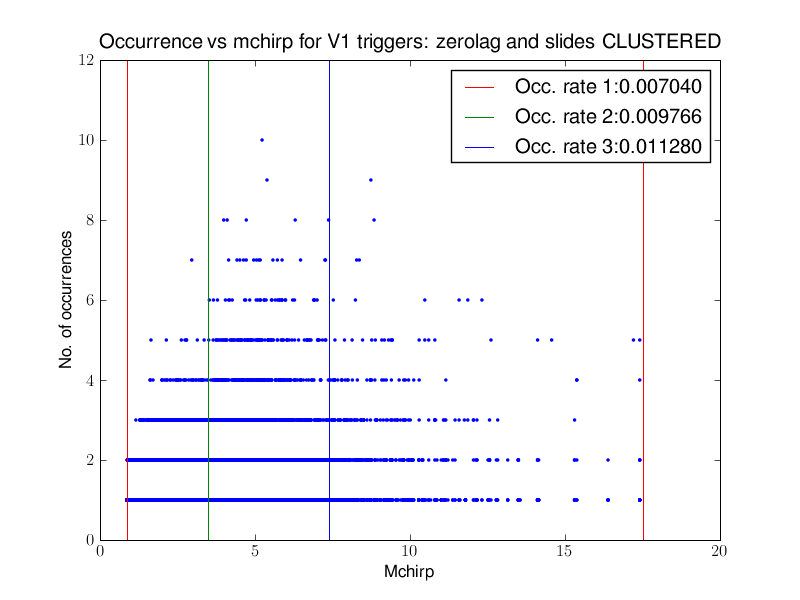
\includegraphics[scale=0.45]{V1_clustered.png}
%\caption{GRB090809B: number of occurrences of V triggers after trial clustering}
%\label{fig:figure4}
%\end{minipage}
\caption{GRB090809B: number of occurrences of L and V triggers (N, counts) versus chirp mass}
\label{occurrencefigures}
\end{figure}

The occurrence rate $z$ of a trigger in coincidences can be defined as the number of times a same trigger shows up in different coincidences with triggers from the opposite detector. The avergae occurrence rate per detector per chirp mass bin $i$ can be written as:

\begin{equation}
\label{occrate1}
z^1_i = x_i R^2_i
\end{equation}
\begin{equation}
\label{occrate2}
z^2_i = x_i R^1_i
\end{equation}

It is useful to look at the trigger occurrence rates $z$ collected from GRB090809B analysis to have an idea of the magnitude order and moreover to look at a comparison between occurrences in timeslides background and in zerolag background. This data is listed in Table ~\ref{occurrences}. The trigger occurrence rates listed in Table ~\ref{occurrences} have been obtained by employing a computer program that simply counts the triggers and their occurrences and does not use the equations (\ref{occrate1}) - (\ref{occrate2}). 

\begin{table}[ht!]
 \begin{tabular}{|l|l|l|l|l|l|}
 \hline
 \hline
 $z_{1}^L$ & $z_{2}^L$ & $z_{3}^L$ & $z_{1}^V$ & $z_{2}^V$ & $z_{3}^V$  \\
 \hline
 0.019 & 0.047 & 0.037 & 0.012 & 0.025 & 0.035 \\
 \hline
 0.012 & 0.037 & 0.026 & 0.004 & 0.018 & 0.026 \\
 \hline
 \hline
 \end{tabular} 
 \caption{GRB090809B: trigger occurrence rates in coincidences for individual L and V triggers for zerolag and timeslides data, in units of Hz}
 \label{occurrences}
\end{table}

The Table ~\ref{occurrences} has two implications:
\begin{itemize}
\item
The first implication is that individual trigger occurrence rates are much higher in the medium and high chirp mass bins. So if a glitch or any unwanted loud trigger has a medium or high chirp mass it will be part of more coincidences than a similar one that has a low chirp mass.
\item
The second implication is that by looking at both the zerolag and the timeslides numbers we see almost to no change , hence equations (\ref{occrate1}) - (\ref{occrate2}) stand fine since they are independent of the number of trials.
\end{itemize}

An alternative way of \emph{estimating} the coincidence window $x$ in the case of GRB090809B is to use equations (\ref{occrate1}) - (\ref{occrate2}) and Tables \ref{rates} and \ref{occurrences}: by averaging over the two occurrence rates per chirp mass bin we get similar results to  the ones in Table \ref{xes} - low chirp mass bin coincidence window $x_1 \approx 2 \times 10^{-4}$, medium chirp mass bin coincidence window $x_2 \approx 5 \times 10^{-3}$ and high chirp mass bin coincidence window $x_3 \approx 5 \times 10^{-2}$.

The probability that a trigger will form $k$ coincidences when doing an analysis comprising $S$ timeslides may be approximated with a Poisson process probability:

\begin{equation}
\label{poissontriggers}
p^{1,2}_i(k, S) = \frac{\sum_l N^{1,2}_l(k, S)}{N_0} \approx \frac{{(z^{1,2}_iS)}^k}{k!} \mathrm{e}^{-z^{1,2}_iS} = \frac{{(x_iR^{2,1}_iS)}^k}{k!} \mathrm{e}^{-x_iR^{2,1}_iS}
\end{equation} 
%
where $\sum_l N^{1,2}_l(k, S)$ represents the summing numbers of different triggers that each shows up in exactly $k$ coincidences, and $N_0$ is the total number of coincidences.

Figures \ref{poissonL} - \ref{poissonV} are histograms of the number of trigger occurrences fitted with Poisson distributions given by (\ref{poissontriggers}) for GRB090809B. The fit is not perfect but is close enough. 

\begin{figure}[ht!]
\begin{minipage}[b]{0.5\linewidth}
\centering
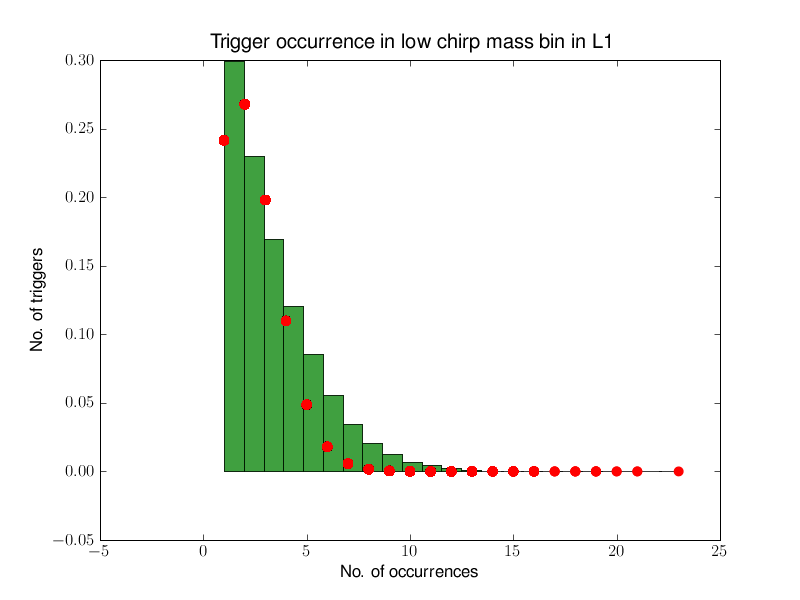
\includegraphics[scale=0.45]{l1_low_distribution.png}
%\caption{Histogram of number of trigger occurrences in coincidences for GRB090809B: detector 1, low chirp mass bin (L1low)}
%\label{figure4}
\end{minipage}
\begin{minipage}[b]{0.5\linewidth}
\centering
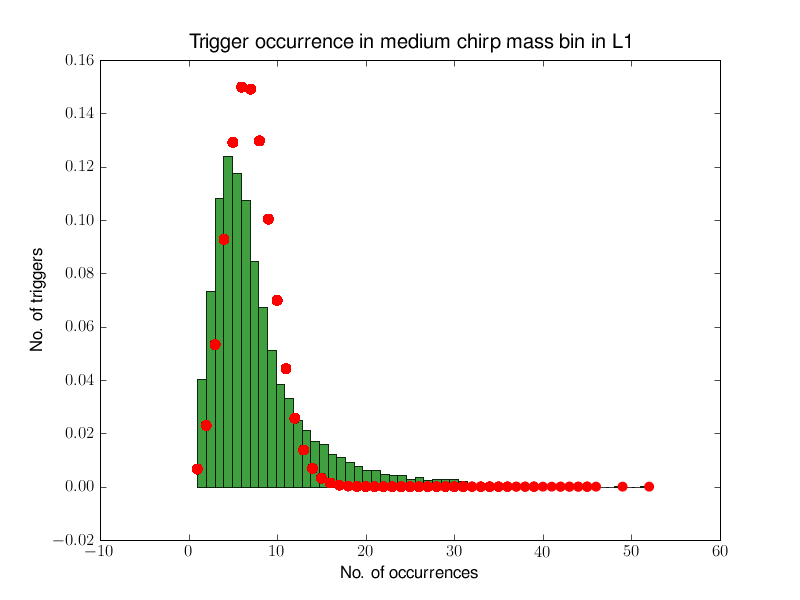
\includegraphics[scale=0.45]{l1_medium_distribution.png}
%\caption{Histogram of number of trigger occurrences in coincidences for GRB090809B: detector 1, medium chirp mass bin (L1medium)}
%\label{figure5}
\end{minipage}
\begin{minipage}[b]{0.5\linewidth}
\centering
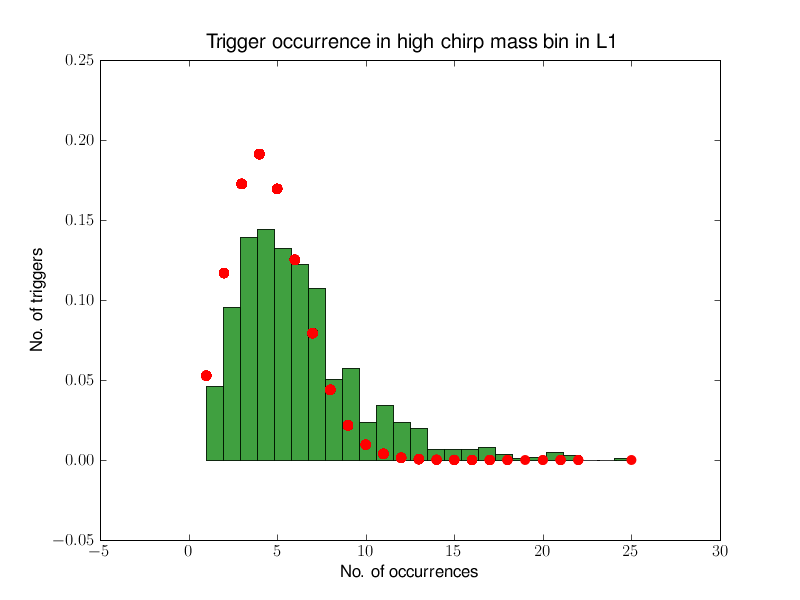
\includegraphics[scale=0.45]{l1_high_distribution.png}
%\caption{Histogram of number of trigger occurrences in coincidences for GRB090809B: detector 1, high chirp mass bin (L1high)}
%\label{figure6}
\end{minipage}
\caption{Histogram of number of trigger occurrences in coincidences for GRB090809B, detector 1 (L): low, medium and high chirp mass bins}
\label{poissonL}
\end{figure}

\begin{figure}[ht!]
\begin{minipage}[b]{0.5\linewidth}
\centering
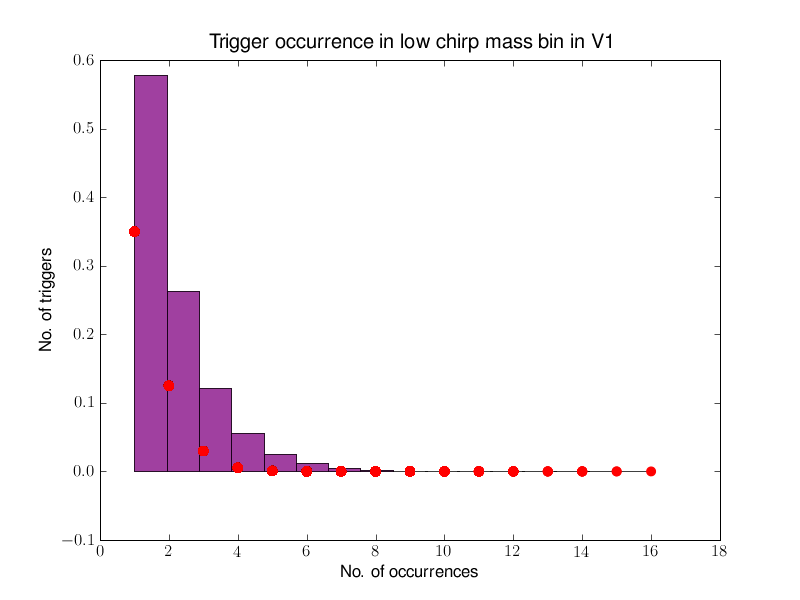
\includegraphics[scale=0.45]{v1_low_distribution.png}
%\caption{Histogram of number of trigger occurrences in coincidences for GRB090809B: detector 1, low chirp mass bin (L1low)}
%\label{figure4}
\end{minipage}
\begin{minipage}[b]{0.5\linewidth}
\centering
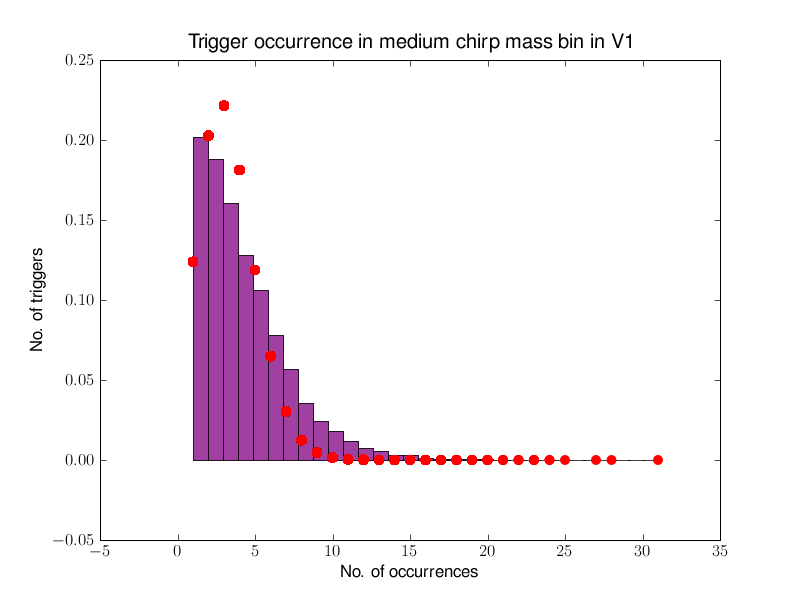
\includegraphics[scale=0.45]{v1_medium_distribution.png}
%\caption{Histogram of number of trigger occurrences in coincidences for GRB090809B: detector 1, medium chirp mass bin (L1medium)}
%\label{figure5}
\end{minipage}
\begin{minipage}[b]{0.5\linewidth}
\centering
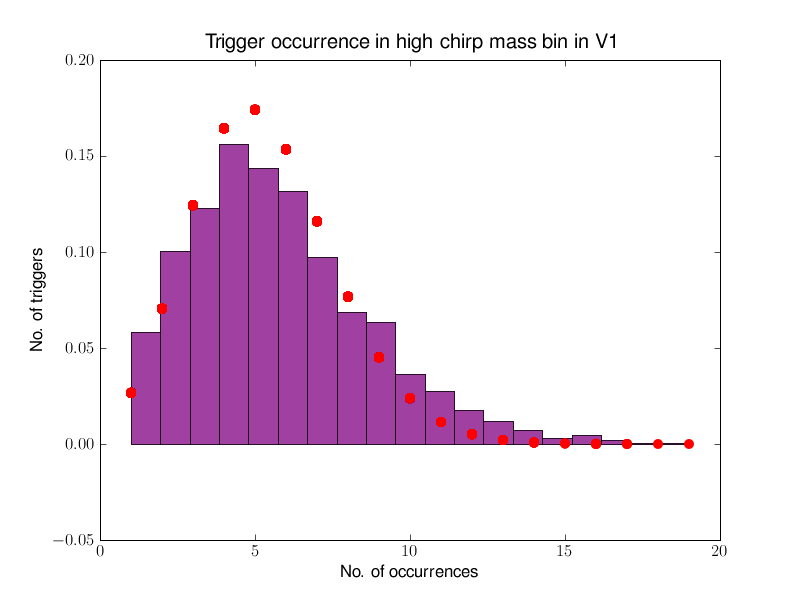
\includegraphics[scale=0.45]{v1_high_distribution.png}
%\caption{Histogram of number of trigger occurrences in coincidences for GRB090809B: detector 1, high chirp mass bin (L1high)}
%\label{figure6}
\end{minipage}
\caption{Histogram of number of trigger occurrences in coincidences for GRB090809B, detector 2 (V): low, medium and high chirp mass bins}
\label{poissonV}
\end{figure}

\paragraph{Finding a conservative upper limit for $S^{\mathrm{max}}$} Equation (\ref{poissontriggers}) approximates the probability of finding a trigger $k$ times in $k$ different coincidences when doing $S$ timeslides. Let's consider the case of the low chirp mass bin for which we take the coincidence window constant across the bin and fixed at $x_1=x=10^{-4}~\mathrm{s}$ and plot the probabilities (\ref{poissontriggers}) for different $k$'s for either detector 1 or 2 as function of rate of either detector 2 or 1 multiplied by the number of timeslides:

\begin{equation}
p^{1,2}_k = p^{1,2}_k(R^{2,1} \times S), ~~~k=\bar{1,N}
\end{equation}

 An example of such plot is shown in Figure \ref{poissonks} for $k$=1,2,3,5 and 10.

\begin{figure}[ht!]
%\begin{minipage}[b]{1.0\linewidth}
\centering
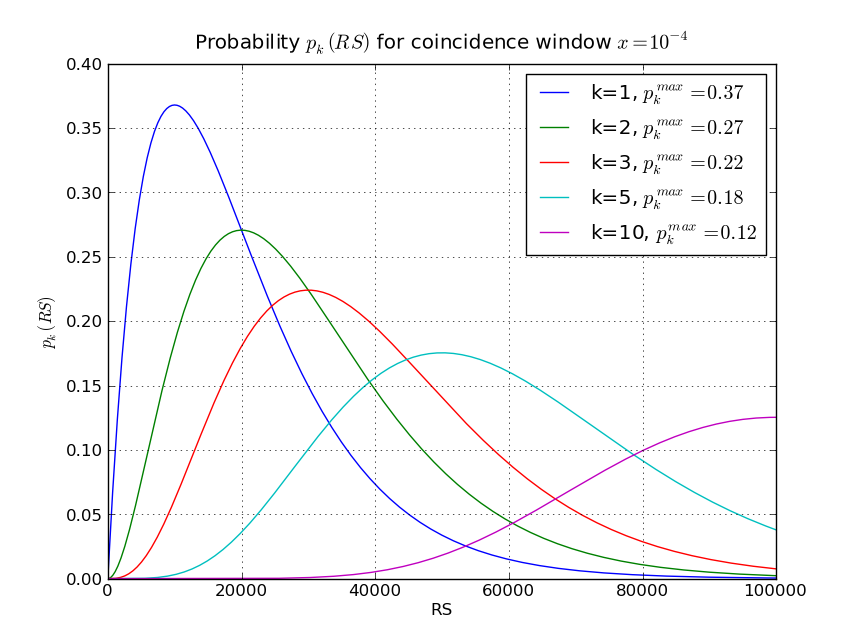
\includegraphics[scale=0.50]{pk_of_RS.png}
\caption{Probability of finding a trigger in $k$ different coincidences function of the $RS$ (Hz) product for different $k$'s}
\label{poissonks}
%\end{minipage}
\end{figure}

In an ideal case the number of times $k$ a trigger forms coincidences should be as low as possible, prefrerably one, \emph{i.e.} every trigger forms one single coincidence and does not get recycled in more coincidences with the incease of number of timeslides. By looking at Figure \ref{poissonks} we can set a conservative limit for $R \times S$ by imposing:

\begin{equation}
p^{1,2}_{k=1}(R^{2,1} \times S) = p^{1,2}_{k=2}(R^{2,1} \times S)
\end{equation}
\begin{equation}
\mathrm{min}(\frac {2}{xR^1}, \frac {2}{xR^2}) ~\leq~ S^{\mathrm{max}}_{\mathrm{lim}} ~\leq~ \mathrm{max}(\frac {2}{xR^1}, \frac {2}{xR^2})
\end{equation}

Ideally, we would want to choose an $S$ to have $p^{1,2}_{k=1}(R^{2,1} \times S) = \mathrm{max}$ hence $dp^{1,2}_{k=1}(R^{2,1} \times S)/d(R^{2,1} \times S)=0$ and that yields a reccommended number of timeslides $S^{\mathrm{max}}_{\mathrm{recc}}$ given the two single detector trigger rates $R^{1,2}$, the coincidence window $x$ and the fact that we want to keep $k=1$:

\begin{equation}
\mathrm{min}(\frac {1}{xR^1}, \frac {1}{xR^2})~ \leq ~S^{\mathrm{max}}_{\mathrm{recc}}~ \leq ~\mathrm{max}(\frac {1}{xR^1}, \frac {1}{xR^2})
\label{timeslidesinterval}
\end{equation}

\paragraph{Threshold SNR} The single detector rates depend intrinsically on the signal-to-noise ratio threshold $\rho_0$, fixed during a certain search. According to \cite{} one can write the functional variation of the rate with threshold SNR:

\begin{equation}
R(\rho_0) = C\mathrm{e}^{-\frac{\rho_0^2}{2}}
\end{equation}

where $C$ is a constant that folds in characteristics of the template bank used during the search.

\subsubsection{Conclusions}

Reiterating the items listed in the introductory section, we find answers to the questions posed to what is the best way to estimate background by doing timeslides in the CBC coincident GRB search:
\begin{itemize}
\item
What is the desired sensitivity of the search, in other words, what is the maximum false alarm rate (FAR) (or probability, FAP) a detection result should be quoted with?

\emph{ANSWER}: By looking at the local rates for short hard GRBs, one would want a FAR that is at most of the same order as the rate so would accept a detection at a FAR of say at most $10^{-4}$.

\item
What is the maximum number of timeslide that one can perform so that one can still gain in senisitivity -- that is, up to what $S^{max}$ can one go so that the FAR (FAP) will still decrease and reach the minimum quoted by answering the above question?

\emph{ANSWER}: The maximum number of timeslides depends on two issues: first, if we do too many timeslides we don't gain anymore in sensitivity (\cite{was}) and second, if we do too many timeslides we risk an oversaturation of triggers in coincidences , that is, the probability that a trigger will form multiple coincidences with a multiplicity $k>1$ will be larger than the same probability for $k=1$. Whereas equation (\ref{timeslidesmax}) may shed light on the number of timeslides up to which the search can still gain in sensitivity, in practice it is found thet usually that $S^{\mathrm{max}}$ is too small to be used. A few times  $S^{\mathrm{max}}$ will be used in practice and an interval for $S$ is given by equation (\ref{timeslidesinterval}). That shows us that the lower the single detector trigger rates the more timeslides one can do. In the standard S6 GRB case we have about 100 to 200 slides in the low chirp mass bin given by equation (\ref{timeslidesinterval}).

\item
How independent will be the resulting coincidences from doing slides, knowing that the timeslides method does not produce new triggers but rather recycles the existing triggers present in the initial stretch of data and rearranges them to create new coincidences? That is, having a Poisson distributed collecton of single detector triggers, that will be creating coincidences, which triggers will be prone to repeat in coincidences more often than the others, if there is any preference towards such a behavior?

\emph{ANSWER}: Single detector triggers follow an almost Poisson distribution in the timeslides coincidences; there has been no priviliged occurrence observed, as function of SNR. Medium  and high chirp mass bin triggers show up more often relative to low mass triggers due to a more loose mass-time coincidence window constraint.

\item
How will a loud trigger/glitch affect the statistics by propagating in coincidence and being the loudest event in coincidence?

\emph{ANSWER}: A loud single detector trigger deemed as background trigger will follow the same statistics as the other triggers. Glitches are a different story.

\item
What is the nominal sensitivity of the search, in other words, what is the maximum false alarm rate (FAR) (or probability, FAP) and its error a detection result should be quoted with, with figures extracted from the statistical properties of the GW data? Is this sufficient, \emph{i.e.} how does it compare to the one quoted by answering the first question?

\emph{ANSWER}: The answer to this question is not exactly an easy one. Say we would tighten the coincidence window to $x=10^{-5}$, decrease the single detector trigger rates to $R \approx 10~\mathrm{Hz}$ and increase the analysis time to $T=4000~\mathrm{s}$. We may use equation (\ref{timeslidesinterval}) to have an idea on how many timeslides to do, that would yield about 10,000 slides - and in this case we are sure that we minimize the repetitivity of triggers in coincidences (the probability in equation (\ref{poissontriggers}) $p_k(R,S)$ is maximum for $k=1$). All of this would give us a $\mathrm{FAR} \approx 10^{-3}~\mathrm{Hz}$ and a $\sigma \approx 10^{-5}~\mathrm{Hz}$ (from equations (\ref{faar})-(\ref{far_variance})-(\ref{fequal})), which is a good starting point.

\end{itemize}


\subsubsection{APPENDIX: Study on four S6A GRBs}

By repeating the calculation steps described above, one can look at other GRBs and in this case the tables below show how the parameters change when looking at four different S6A GRBs.

\begin{table}[ht]
 \begin{tabular}{|l|l|l|l|l|l|l|l|}
 \hline
 \hline
 GRB & IFOs & $R_{1}^L$ & $R_{2}^L$ & $R_{3}^L$ & $R_{1}^V$ & $R_{2}^V$ & $R_{3}^V$ \\
 \hline
 090709B & L1V1 & 57.59 & 9.06 & 1.16 & 125.11 & 8.86 & 0.65 \\
 \hline
 090727 & L1V1 & 51.38 & 7.26 & 1.03 & 112.75 & 9.43 & 0.82 \\
 \hline
 090809B & L1V1 & 39.41 & 4.31 & 0.68 & 122.15 & 8.98 & 0.68 \\
 \hline
 090814B & L1V1 & 60.35 & 9.31 & 1.1 & 127.91 & 10.77 & 0.86 \\
 \hline
 \hline
 GRB & IFOs & $x_1$ & $x_2$ & $x_3$ & $S^{max}_1$ & $S^{max}_2$ & $S^{max}_3$  \\
 \hline
 090709B & L1V1 & 0.00019 & 0.0091 & 0.1061 & 30 & 7 & 5 \\
 \hline
 090727 & L1V1 & 0.00013 & 0.0047 & 0.0474 & 50 & 13 & 12 \\
 \hline
 090809B & L1V1 & 0.00009 & 0.0046 & 0.0346 & 70 & 17 & 21 \\
 \hline
 090814B & L1V1 & 0.00014 & 0.0058 & 0.063 & 40 & 9 & 8 \\
 \hline
 \hline
 \end{tabular} 
 \caption{Four S6A GRBs and their numbers}
 \label{Table 3}
\end{table}

\begin{table}[ht]
 \begin{tabular}{|l|l|l|l|l|l|l|l|}
 \hline
 \hline
 GRB & IFOs & $z_{1}^L$ & $z_{2}^L$ & $z_{3}^L$ & $z_{1}^V$ & $z_{2}^V$ & $z_{3}^V$  \\
 \hline
 090709B & L1V1 & 0.024 & 0.081 & 0.069 & 0.011 & 0.082 & 0.123 \\
 \hline
 090727 & L1V1 & 0.015 & 0.044 & 0.039 & 0.007 & 0.034 & 0.049 \\
 \hline
 090809B & L1V1 & 0.011 & 0.041 & 0.024 & 0.004 & 0.020 & 0.024 \\
 \hline
 090814B & L1V1 & 0.018 & 0.062 & 0.054 & 0.008 & 0.054 & 0.069 \\
 \hline
 \hline
 \end{tabular} 
 \caption{Expected occurrence rates in coincidences of individual L and V triggers for the four S6A GRBs (Hz)}
 \label{Table 3}
\end{table}

By averaging the values in the tables (even though the statistical sample of four GRB is not yet enough, but it is a good indicator still) one can get a table with the take-home values for the parameters we would be interested in:

\begin{equation}
<x_1> = 0.00014 s, <x_2> = 0.0061 s, <x_3> = 0.063 s
\label{xs}
\end{equation}
\begin{equation}
<S^{max}_1> \sim 50, <S^{max}_2> \sim 12, <S^{max}_3> \sim 12
\end{equation}
\begin{equation}
<R^L_1> \sim 52 Hz, <R^L_2> \sim 7.5 Hz, <R^L_2> \sim 1 Hz
\end{equation}
\begin{equation}
<R^V_1> \sim 122 Hz, <R^V_2> \sim 9.5 Hz, <R^V_2> \sim 0.75 Hz
\end{equation}


\subsection{Future work}
 Data analysis from the S6/VSR2 GRBs will be performed in a semi-automated mode. I have already volunteered to be part of the GRB effort for S6/VSR2 science run and this will transcribe in a better understanding of the GRB inspiral code and continiously improving both the analysis and post=processing stages. Also, whenever the automated analysis fails, I will try and analyze the data (as described above) manually. I have already been assigned with improving the manner in which the timeslides are performed and this will continue in the future with other pipeline improvements. 


 
\section{Perspectives on joint detection of GW and radio transients}

\subsection{Introduction}

Many
potential sources of transient gravitational wave (\gw) signals may emit
electromagnetic counterparts detectable by existing and planned astronomical instruments.
The coincident detection of an electromagnetic signal may provide
some of the most compelling evidence for the unambiguous direct detection of
gravitational waves, as well as provide important information on the
nature of the progenitor system.  Short, hard $\gamma$-ray bursts (GRB) provide a typical
example of such a scenario.  These are believed to be the electromagnetic signatures of
the coalescence of a compact binary system, consisting of two neutron stars (NS) or
a neutron star and a black hole (NS-BH).  Gamma ray bursts have been used quite extensively
to trigger \gw searches for some time~\cite{Abbott:2007rh,Collaboration:2009kk,0264-9381-25-22-225001}
and, indeed, a recent search for \gws from a GRB initially associated with the Andromeda galaxy
was able to confidently exclude a compact binary coalescence at the distance of M31 due to the absence
of significant \gw emission~\cite{Abbott:2007rh}, but did not exclude a binary coalescence event at larger distances.

Searches for \gws which are {\emph triggered} by electromagnetic observations possess
several advantages over un-triggered all-sky searches.  Typically, an all-sky
search is performed over an entire science run, lasting weeks to months and
must search all sky locations for putative gravitational wave signals. An
electromagnetically triggered search, by contrast, is usually performed
over a much shorter time window lasting a few to several hundred seconds,
depending on the nature of the trigger, and the sky--location of the source is
usually also known to high precision.  The smaller time window increases the search
sensitivity since there will be a smaller number of instrumental and terrestrial
artefacts in the data, allowing one to tolerate signal detections with lower
significance than would be the case for a longer duration search.  Knowledge of 
the expected time of the gravitational wave signal allows one to make a distinction
between {\emph on} and {\emph off--source} data.  The off-source data, typically
taken soon before and soon after the trigger is used to estimate the background
rate of potential gravitational wave triggers and the statistical significance
of detection candidates in the on--source data.   Since the noise from
gravitational wave detectors is generally non-stationary, it is important that
the data used for background estimation is taken near to the trigger to accurately
reflect the noise properties of the on--source data.  This, however, is
generally not problematic due to the fairly short on--source windows used in
externally triggered analyses.  As well as the gain in sensitivity from the short
on--source window, the sky--location used in electromagnetically triggered
searches provides more robust signal--consistency tests in multi-detector searches
and significantly reduces the parameter space of the signal.

Observations in radio astronomy have already had a significant impact on
the search for gravitational waves.  Most significantly, the accurate
timing of pulsars in radio has enabled searches for gravitational wave
emission from known pulsars \cite{known_pulsars}.  These radio
observations permit a significant reduction of the gravitational wave
parameter space, resulting in a more sensitive search.
Recently, the gravitational wave emission from the Crab pulsar has been
bounded to be significantly below the spin-down limit \cite{crab}.  In
addition, observations of pulsar glitches \cite{Flanagan:2006,Buchner:2008} have prompted
searches for gravitational waves emitted at the time of the glitch~\cite{Clark:2007}.

In this paper, we advocate the extension of the joint radio and
gravitational wave search effort to include transient signals in the
radio band.  Until now, there have been no completely systematic searches for transient radio
signals but there are tantalising hints of a significant population of transients
\cite{Lazio:2009xe} which a new generation of radio telescopes and
arrays are ideally positioned to observe.  Given the nascent state of
the field, there is great uncertainty regarding the nature of the progenitor of 
many radio transients. Several of the proposed sources of radio transients are
also expected to be strong and, in some cases, well-modelled sources of 
gravitational waves.  The potential for serendipitous discovery
of new gravitational wave and radio sources, as well as the existence of 
theoretically modelled mechanisms for radio emission associated with known classes of
astrophysical objects, provide strong motivation for proposing a joint
gravitational wave and radio observation effort. On top of this, the astrophysical 
information encoded in the radio and gravitational waveforms will likely be complementary.
Thus, as with many multi-wavelength or multi-messenger observations,
combining the data from these two different observing channels will
enhance the astrophysical understanding of the source.

\subsection{Search tools: radio telescopes and gravitational wave interferometers}
\label{sec:telescopes}

\subsubsection{Radio telescopes and recent radio transients survey activity}
\label{ssec:radio_tele}

Radio telescopes fall into two categories --- dishes and aperture
synthesis arrays. We begin by enumerating in Table \ref{tab:radioinst}
some of the key specifications of radio telescopes proposed for use in
relation to coincident searches and follow-up in more detail on
a number of previewed telescopes to be used in the very first stages of
the search.

\begin{table}[h!]
\begin{center}
\begin{tabular}{|l|l|l|l|l|}\hline
Instrument & Band & Max. sensitivity & Field of View & Slew Time\\ \hline \hline
LOFAR & 40-240\,MHz & 2.2 mJy & 186 $\mathrm{deg^2}$ & Software \\ \hline
ETA & 29-47\,MHz & 10 Jy &  $\sim$ 400 $\mathrm{deg^2}$& Software \\ \hline
NRAO Green Bank & 1.15-1.73 GHz & $\sim$ 1 mJy &
0.027 $\mathrm{deg^2}$ &  $18^\circ$/minute\\ \hline
Arecibo & 312\,MHz - 10.2\,GHz & $\sim$ 0.5 mJy &
0.063 $\mathrm{deg^2}$ & $<16$\,min\\
%(ALFA) & 1.225 - 1.525 GHz &  &
%10\,arcmin (7 beams)
%& \\

\hline
\end{tabular}
\end{center}
\label{tab:radioinst}
\caption{Observational capabilities of some of the radio telescopes proposed for a joint GW-radio search effort.} \footnotemark
\end{table}
\footnotetext{The aperture synthesis arrays like LOFAR and ETA have wide fields of view operating in relatively narrow frequency bands whereas the single dish telescopes like NRAO Green Bank and ARECIBO have significantly decreased fields of view but can operate within much broader frequency bands. Radio flux sensitivity is given in Jansky (1 Jy=$10^{-19}\,\mathrm {erg}\,\mathrm{m^{-2}\,\mathrm {s^{-1}}\,\mathrm{Hz}}$). The slew time is how fast the telescope can turn around its symmetry axis to track a sky location.}

\paragraph{Low Frequency Array (LOFAR)} 
LOFAR is a UHF antenna array recently commissioned by a Dutch consortium
lead by the Netherlands Institute for Radio Astronomy (ASTRON) and the
University of Groningen. The instrument has made its first observational
trials at the end of August 2009 and according to the latest news from
\cite{Garrett:2009gp} the first international observational effort has
just been completed. The instrument and the capabilities afforded by the
design are discussed elsewhere \cite{lofar_case}. Briefly, the design
calls for the deployment of 41 ground stations centered in the
Netherlands and further stations extending throughout western Europe.
Each ground station comprises of an array of sensors, including between
48 and 96 each of ``low-band'' and ``high-band'' antennae\footnote{International stations further from the core group in
the Netherlands will add more antennae.} having usable bandwidths of
30-80\,MHz and 120-240\,MHz respectively and a maximum sensitivity of
10\,mJy.  One of the key science projects of LOFAR is to search for
radio transients.  Potential sources include X-ray binaries, GRBs, SNe
and AGN. 

\paragraph{Eight-meter Transient Array (ETA)} 
The Eight-meter-wavelength Transient Array \cite{Patterson:2008ie} has been
constructed and operated by researchers at Virginia Tech.  This
instrument is designed specifically to detect low-frequency radio
transients, covering the band 29--47 MHz with full-bandwidth sampling.  Its
flexible signal processing system supports a number of modes by phasing
its individual dipole antennas, but it will typically be operated with
two 30-degree-wide synthesized beams to do a broad continuous search.

\paragraph{Green Bank NRAO} 
The Green Bank Telescope (GBT) is the world's largest fully steerable
radio telescope \cite{Mason:2009dq}. GBT is located at the National Radio Astronomy
Observatory's site in West Virginia, USA. GBT is a 100-meter telescope
on a wheel-and-track design that allows the telescope to view the entire
sky above 5 degrees elevation.  

\paragraph{Arecibo}
The Arecibo radio telescope in Puerto Rico, USA, is the world's largest
and most sensitive radio telescope (312\,MHz - 10.2\,GHz and 0.5\,mJy
sensitivity \cite{Lommen:2000yt}).  It is part of the National Astronomy and Ionosphere
Center (NAIC) operated by Cornell University.  The telescope itself
consists of a 305 meter diameter fixed primary reflector, with a
suspended platform containing secondary and tertiary reflectors along
with various receivers.  The telescope can be pointed within $20^\circ$
of zenith by moving the suspended platform, with a slew rate of
$24^\circ$/minute in azimuth and $2.4^\circ$/minute in zenith angle.
The secondary and tertiary reflectors correct for spherical aberration.


\paragraph{}
Systematic surveys of the transient radio skies are expected to be performed in the near future at a greater rate than in the past \cite{Lazio:2009xe}. The unexpected results from such past surveys include discoveries of completely new radio sources (e.g. Rotating Radio Transients,~\cite{BurkeSpolaor:2009rm}). 
As an example, in the summer of 2007 Green Bank Telescope took a survey of the
northern sky at 350\,MHz which covered 12,000 sq degrees. This survey~\cite{Hessels:2007ct} was
called the drift-scan survey because it was done while the azimuth track
was being refurbished. Data from this survey has thus far uncovered 25
new pulsars including 5 new millisecond pulsars.  This data is still
being searched for new pulsars and radio transients. This shows the
shear diversity and abundance in new radio sources that can be uncovered
by doing a rather short but systematic survey and reveals the potential
of a multi-messenger search. 


\subsubsection{Gravitational wave interferometers}
\label{ssec:gw_det}

A global network of gravitational wave
interferometers has now been constructed and is taking data.  The instruments
constituting this network
include the Laser Interferometry Gravitational Observatory (LIGO), which operates two
observatories in the USA~\cite{Abbott:2007kv}; the French-Italian Virgo detector~\cite{Virgo_status}, based in Italy; the
British-German GEO600 detector in Germany~\cite{GEO_status} and the TAMA300 detector in Japan~\cite{TAMA_status}.  Data
from these detectors has been acquired and analyzed over the past
decade.  These detectors have achieved or come close to their design
sensitivities, and an extended science run of the
LIGO, GEO and Virgo detectors was completed over 2005 to 2007 (known as S5 in
LIGO/GEO and VSR1 in Virgo).  The detectors achieved a strain
sensitivity of better than $10^{-22}/\sqrt{\mathrm{Hz}}$ at their most
sensitive frequencies (around $100$ Hz).  This can be translated into
sensitivities to various sources, for example the LIGO detectors in S5
were sensitive to optimally oriented and located (i.e. overhead the
detector) binary neutron star signals to a distance of $35$ Mpc, and hundreds of Mpc for
more massive compact binary coalescences.  For short-duration, narrow-band transients,
such as the \gw signal one may expect from core-collapse supernovae,
this sensitivity corresponds to a gravitational wave energy as low as
$10^{-8} M_{\odot}c^2 \sim 2 \times 10^{46}$~erg for galactic events and $0.1 M_{\odot}c^2 \sim 2 \times 10^{53}$~erg for events in
the Virgo cluster at 16 Mpc.

Following the S5/VSR1 run, the LIGO and Virgo detectors have been
technically upgraded to enhanced configurations, and the latest science run
(S6/VSR2) began in the summer of 2009, aiming at collecting data at better sensitivities than S5/VSR1.  Following this data taking
period, both LIGO and Virgo detectors will be upgraded to advanced
configurations with approximately ten times the strain sensitivity of
the initial detectors.  For sources distributed uniformly in volume,
this corresponds to a sensitivity to a thousand times as many sources.
In terms of energy, the sensitivity will be $\sim 10^{-10} M_{\odot}c^2 \sim 2 \times 10^{44}$~erg
for galactic events.  The advanced detectors are expected to begin
acquiring scientific data by 2015. 

\subsection{Radio and Gravitational Wave Sources} 
\label{sec:sources}

Joint observation of gravitational waves and their radio afterglow
requires a mechanism for the prompt generation of a radio counterpart to
the gravitational wave signal. Furthermore, to avoid self-absorption by
the source, models yielding coherent radio emission are favoured.  The
prospects for detecting gravitational waves from a given progenitor
depend on the details of the underlying engine, which in many cases are
still uncertain.  To pursue a joint radio and GW analysis, one requires
a reliable estimate of the delay between the gravitational and radio
waves, given by the dispersion measure of the media in which the wave
travels.  There are several possible progenitors for emission in both
gravitational and radio waves, two of which are discussed below:
coalescing neutron star binaries and short hard GRB afterglows.  We
conclude this section with a brief discussion of the effects of
dispersion on the radio signal. 

\subsubsection{Neutron Star Binaries}

Binary neutron stars are one of the most promising candidate for
gravitational wave sources.  Indeed, the observations of several binary
pulsars provide strong evidence for the emission of gravitational waves
from these systems \cite{weisberg:2004}, as well as an estimate of the
rate of such coalescences in the nearby universe \cite{Kalogera:2004tn, Kalogera:2004nt}.  The
waveform emitted by a coalescing neutron star binary system has been
calculated to great precision in the post-Newtonian formalism
\cite{Blanchet:2002av}.  Initial and enhanced detectors are sensitive
to the signal to tens of Mpc while the advanced detectors will be sensitive
to hundreds of Mpc.  Several gravitational wave searches for coalescing
neutron star binaries have already been performed \cite{Collaboration:2009tt,
Abbott:2009qj}. At the time of writing, there has been no confirmed direct
detection of \gws using purpose-built detectors.  However, the 
upper limits obtained on the rate of binary coalescences are now approaching 
those predicted by astrophysical arguments.  The expected rate of such coalescences
observed in the advanced LIGO and Virgo network is expected to be tens
per year.

There are a number of models for the emission of radio
waves during the late stages of a compact binary inspiral phase or during their coalescence,
making these an ideal source for joint radio-GW searches.  We
discuss two classes of radio emission models below, based on the predicted emission mechanism.

\paragraph{Radio emission due to strong magnetic fields}

The first class of models
require one of the neutron stars to possess a large magnetic field
($10^{12} - 10^{15}$ ~G). This type of neutron stars, called magnetars, represent a fraction of 10 $\%$ of the known population of neutron stars \cite{Bogomazov:2009wj} and 18 have been discovered of which eight are Soft Gamma Repeaters (SGRs) and ten are Anomalous X-ray Pulsars (AXPs) ~\cite{magnetar_catalog}, all of them isolated objects. According to \cite{Popov:2005wh} binary systems with a magnetar and a compact companion may account for 1 $\%$ of the total number of neutron stars in the universe. 


The model described in \cite{Lipunov:1996wf} assumes the binary
neutron star system is composed of stars with (approximately) equal
masses and radii in the final stages of inspiral.  One of the two NS
is required to be a magnetar, with magnetic field
$B\sim10^{12}-10^{15} \mathrm{G}$, with the second star's magnetic
field significantly weaker.  Their spins are neglected.  By
modelling the stars as perfect conducting spheres, it can be shown
that as the companion orbits in the magnetic field of the magnetar,
a magnetic dipole is induced in the companion and
dipolar radiation is emitted.  The expected in source luminosity is given by ~\cite{lipunovflux}

\begin{equation}
\label{lipunovflux}
L_(t) = \frac{8\mu^2 \sin^2\alpha \omega_{orb}^8}{3c^3\omega_{cr}^4}
   \sim 5\cdot 10^{32}\sin^2\alpha\mu_{30}^2 t^{-3}\mbox{ erg s}^{-1}
\end{equation}

where $\omega_{cr} = \sqrt{GM/R^3}$ and $R$ is the star's radius.
 The maximum luminosity is of the order
of $L_{max}\sim 10^{41}\,\mathrm{erg/s}$. It is thought that, in
analogy with the pulsar model, a fraction of this energy will be
radiated in radio band with an observable flux equal to the flux from the Crab pulsar (PSR B0531+21) at a distance of 2 Mpc. The Crab pulsar is located at a distance of 2kpc ~\cite{ATNF} and its radio flux at the 400 MHz pulsar reference frequency is 650 mJy ~\cite{Nice:1998dn}. For a source placed at 100 Mpc, this model would predict a radio flux of $\mathrm{F_{\nu}}\sim 0.3\, \mathrm{mJy}$ at a frequency of 400 MHz, too low for a detection, but for sources at 10 Mpc or less the flux would be within the detection range of existing radio telescopes.  



In a second model \cite{Hansen:2000am}, the magnetar's companion is
assumed to be a rapidly spinning recycled pulsar \footnote{A recycled pulsar is a pulsar with a very short spin period $\mathrm{P}
\sim 1-100$ ~ms, low magnetic field and low spin-down rate, often found in a binary system; recycled pulsars are pulsars which have lost energy and spun down, and then been spun up again by forming a binary system with a companion.}. The magnetar is a
non-recycled slow-spinning pulsar ($\mathrm{P} \sim 10-1000$ ~s). As before,
the orbital and rotational motion of the companion result in an
induced dipolar electric field on its surface.  The majority of the
energy lost by the neutron star is converted into plasma, and later
radiated.  Given the lack of a complete theory for the emission, the
authors assume that $\epsilon \sim 0.1$ of the initial beam energy
is radiated in radio band at a reference frequency of 400 MHz (this
frequency and efficiency are chosen in analogy with radio pulsar
observations).  The maximum luminosity would be $\mathrm{L_{max}}\sim 10^{35}\,\mathrm{erg/s}$, a maximum observable flux of the order
$\mathrm{F_{\nu} \sim 2\,mJy}$ for a source placed at 100 Mpc. The radiation is thought to be emitted isotropically with a spherical symmetry around the low-field companion, so no collimation is assumed.


\paragraph{Plasma excitation through relativistic magnetohydrodynamics}

It is well known (see
e.g.~\cite{Duez:2005sg,Duez:2005sf,Moortgat:2005fs,Moortgat:2004xz})
that, within relativistic magnetohydrodynamics (MHD), gravitational
waves will generically cause excitations of waves in the fluid.
Specifically, it will excite three wave modes in the fluid: Alfven
waves, fast and slow magnetosonic waves.  Thus, in
astrophysical situations with strong gravitational waves travelling
through strongly magnetized plasmas ~\cite{Moortgat:2004xz}, energy
can be transferred from the gravitational field to the plasma.
However, the MHD modes are initially excited at the same frequency
as the emitted gravitational waves.  The challenge then is to
determine whether there will be sufficient up-conversion to higher
frequencies that the energy might escape as electromagnetic
radiation.

In \cite{Moortgat:2005fs,Moortgat:2004xz} the authors argue that
this process could lead to an observable radio signal associated to
binary neutron star coalescences.  The inverse Compton scattering of
the MHD wave by a relativistic ouflow of secondary particles will
lead to the emission of radiation.  When the binary is close to face
 on to the observer, this radiation will be observed at radio
 frequencies, within the sensitive band of the future radio array detectors.
 The nature of the signal predicted in~\cite{Moortgat:2005fs} is an
 incoherent burst of radio waves at 30 MHz with a bandwidth
 of 30 MHz, an in-source power of $\mathrm{P} \sim 10^{47}\,\mathrm{erg/s}$,
 and a duration of roughly 3 minutes. For a source located
 in the Virgo cluster ($\sim 16\,\mathrm{Mpc}$) the predicted fluxes lie in the
 $\mathrm{F_{\nu}} \sim 10^6 \,\mathrm{Jy}$ region.
 Due to the very efficient damping mechanisms predicted in parallel to this
 model, the detected flux will most probably be much smaller, but
 still within the sensitivity of LOFAR. Also, the authors of the model
 consider the electromagnetic radiation to be collimated with a normal
 vector parallel to the normal at the plane of the binary. A lack of
 collimation would render the radio emission invisible to LOFAR.

It is worth mentioning that these two phenomenological model categories do not exclude each other: radio emission due to the presence of a highly magnetized neutron star and its subsequently induced magnetic and electric fields is predicted to occur before the binary merger, wheres interactions of gravitational waves with the surrounding post-merger plasma and consequent MHD phenomena will trigger a radio signal after the merger. 


\subsubsection{Gamma ray bursts}

The coalescence of a binary neutron star or neutron star-black hole system
is still the main candidate progenitor of short hard gamma ray bursts (SHB).  Also, such mergers produce much stronger gravitational wave
emission than other predicted sources, making them some of the most promising candidates for gravitational-wave
detections with the first or second generation of ground-based detectors. The afterglows of SHB have been observed in different wavelengths.   
Short hard GRBs are known for their weak afterglows, making it difficult to secure confirmation of the
progenitor. Results have been published on radio afterglows for short hard bursts but
the data shows only weak signals hours or days after the burst ~\cite{Ofek:2006pr,Soderberg:2006bn}.  

Several authors \cite{Moortgat:2003jh,Usov:2000yr,nakar07} have argued
in favour of a radio component of afterglows from short GRBs, namely a radio burst several minutes after the
observed GRB.  This radio burst is predicted to be a result of synchrotron emission of the electrons in the post-merger plasma and is thought to have a flux on the order of mJy, which is within the sensitivity of current radio telescopes.  In
fact, a proposed discriminant \cite{nakar07} of baryon-dominated (as
opposed to magnetic-field-dominated) outflows is the presence of a radio
flare, stronger than the early optical afterglow, within the first half
hour after the burst. The collimation of the radio burst may be an important factor in observing gamma-orphan bursts (in the case that the orientation of the gamma ray burst is not favorable for a $\gamma$-detection). The authors of \cite{Hansen:2000am} suggest a spherical emission surface whereas \cite{Moortgat:2003jh,Usov:2000yr} consider that the radiation process is highly directional along the gamma-ray emission axis.


Core collapse within massive stars is one of the most widely predicted sources of
transient gravitational and electromagnetic radiation.  This is the underlying
mechanism of supernovae, which occur a few times per century in galaxies
like our own.  At higher masses this collapse can produce long gamma-ray
bursts, which are observed at a rate of $10^{-7}\,\mathrm{yr}^{-1}$ per
galaxy, though the intrinsic rate is likely one or two orders of
magnitude higher due to beaming~\cite{Sadowski:2007dz}. However, the strength of
gravitational-wave emissions from supernovae is quite uncertain.
Optimistically it could be as high as $10^{-4}M_\odot c^2 \sim 2 \times 10^{50}\,\mathrm{erg}$ of energy
released as gravitational waves between 500 and 1,000 Hz
\cite{ott:201102}. Gamma-ray bursts may produce highly-beamed radio bursts within minutes of the gamma-ray burst~\cite{Usov:2000yr}, and supernovae in
general may produce electromagnetic afterglows starting hours after the
initial energy release.


\subsection{Unidentified radio transients}

There is a series of unexplained or poorly understood radio
transients, all documented in the literature.  A few of them have
been located near the galactic center and now bear the name Galactic
Center Radio Transients or GCRT. They are relatively energetic and
bursts have been detected within the 300 MHz frequency region.
Amongst them, GCRT J1745-3009 is a periodic radio transient that
emits $\sim$ 1 Jy pulses with a duration of about 10 minutes every
77 minutes \cite{hyman}.  There are a number of proposed
explanations of this burst, including \cite{turolla} the possibility
that the bursting radio source GCRT J1745-3009 is a binary neutron
star system, with at least one pulsar.  Alternatively, it has been
suggested that this source is a freely precessing pulsar
\cite{zhu}.   

A truly mysterious single transient was observed by Lorimer et al.\
\cite{lorimer} in 2001. At a frequency of 1.5
GHz and less than 5 ms long (believed to be intrinsically shorter,
duration increases due to dispersion), this extremely bright
transient was located at less than 1\,Gpc distance and no host galaxy,
GRB or supernova was associated with its sky location.  It was
detected by the Parkes telescope and based on the telescope's sky
coverage the rate of such events could be as high as 200/day. This
rate gives an unprecedented density of events for a joint
observation effort.

\subsection{Dispersion in the intergalactic and interstellar media and Compton scattering}
Radio waves are strongly coupled to charged
particles and, therefore, are potentially subject to the effects of 
self-absorption in ionized material surrounding the source and to dispersion 
in the interstellar and intergalactic media (ISM and IGM, respectively). 
Self-absorption effects are more pronounced when the radio emission 
is incoherent, as with some of the above emission scenarios associated with
binary neutron star systems.

Following~\cite{pulsar_book}, a radio pulse traveling
in the ionised ISM is delayed over its propagation time through 
free space by a time $\Delta t_{\rm delay}$,
\begin{equation}
\Delta t_{\rm delay} = 4.1\,{\rm ms}\,{\rm DM}~\nu^{-2}_{\rm GHz},
\end{equation}
where $\nu$ is the observation frequency and DM is known as the dispersion measure.
This is the integral along the 
line-of-sight of the electron density between the the observer and the source:
\begin{equation}
{\rm DM} \equiv \int {\rm d}r~n_e(r),
\end{equation}
where $r$ is the distance to the source and $n_e(r)$ is the electron number
density at $r$.

Now, the IGM has a much lower electron number density than the ISM, but the
radio signal must travel a far greater distance through the IGM ($\sim 100$\,Mpc
for advanced detectors) than through the ISM where the emission must propagate across
only $\sim 10$\,kpc for galaxies similar to the Milky Way. In the plane of
the Milky Way, the number density of electrons is, on average, about
$\mathrm{n_e=0.03\,cm^{-3}}$~\cite{thompson}.  So the dispersion
measure for 10\,kpc of ISM equivalent to the disc of
the milky way is $\mathrm{\sim 300\,pc\,cm^{-3}}$.  The expected dispersion
measure contribution for intergalactic distances is $\mathrm{DM} \approx 
100$\,pc\,cm$^{-3}$~\cite{skadoc,palmer} and so the dispersion due to the intergalactic and
interstellar media along the signal path are comparable.  The time
delay due to dispersion for a 1\,GHz radio signal is estimated to be
less than 4\,s for sources within range of advanced detectors \cite{laz}.
Taking this number and adding a component for dispersion in the
interstellar medium, we can estimate that dispersion delays of order
a few seconds for sources embedded in Milky Way-like galaxies at
distances of order a few 100\,Mpc may be expected.
Since the time delay is inversely proportional to the second power of frequency,
lower-frequency signals may be delayed by many minutes; however, the
time of emission may still be inferred from a broadband signal by
extrapolating the delay-vs.-frequency function to infinite frequency.
We therefore retain the benefits of a triggered search.

In the case of short hard GRB radio afterglows, apart from dispersion, the radio waves emited by such bright sources may suffer from induced Compton scattering within the source, phenomenon that will cause a significant dampening of the signal. Detailed in~\cite{Macquart:2007kv}, the induced Compton scattering is the main limiting factor when the region around the progenitor is not dense but when one still considers the scattering effect of a tenuous circumburst interstellar medium. The presence or absence of a radio emission provides an excellent constraint on the Lorentz factor of the GRB outflow during the very early stages of its outburst, hence providing information on the energetics of the progenitor and its nature. 


\subsection{Joint radio-GW searches}
\label{sec:search}

There are two ways in which the coincident detection of a radio--GW
event can be made: either by following up radio transients in existing
gravitational wave data, starting with existing radio transients
detected during the past and present science runs, or by using the
prompt detection and localization of gravitational waves as initial
trigger and {\it alerting} the radio telescopes to point in the
direction where the gravitational wave was observed.  We will discuss
each of these in turn.


\subsubsection{Follow-up of radio transients in archived gravitational wave data}

As we have argued earlier, performing an electromagnetically triggered
search of gravitational wave data has several advantages over the all
sky, all time searches.  The external trigger allows for a significant
reduction in the data to be searched, both by restricting the time
duration and also the sky position.  This reduction in parameter space leads
to a corresponding increase in the sensitivity of the search.  Given the
theoretical models presented in the previous section, there is a clear
motivation for performing a follow-up observation in gravitational wave
data of radio triggers.  Gravitational wave data is routinely archived and also, 
there is no inherent time restriction in performing the search. Indeed, if there
are radio transients identified at times that overlap previous
gravitational wave detector science runs, it is possible and much desired to
search the gravitational wave data around these times.

An outstanding challenge is to obtain a better understanding of the
relative timing of the radio and GW signals.  Once the GW time window is
greater than a few hours, much of the benefit of performing a follow-up style
search is lost.  Thus, it is imperative that we improve our
understanding of the various models presented above to obtain good
estimates of timing differentials between GW and radio signals.  An
interesting aspect of the follow-up of radio triggers is that for each event
we will have an estimate of the dispersion measure.  By measuring the
dispersion, it should be possible to correct for any time delay of the
radio signal.  Furthermore, this should provide an independent
measure of the distance, which could be compared with any GW
observations.

The follow-up searches begin with a list of radio transients; for each
one a GPS time, the duration, the energy of the burst, the dispersion
measure and sky location are recorded. For each event, we advocate the use all available
LIGO/Virgo data at the time of the event to follow-up these events.
Given the source models discussed in section \ref{sec:sources} we
propose the following gravitational wave searches:

\begin{itemize}

\item Search for compact binary coalescence.  There is an argument to
focus this search on binary neutron star signals.  It should be straightforward to apply
a very similar search method to that used for searching for
gravitational waves associated to short GRBs \cite{Abbott:2007rh}.  Although
there are fewer models predicting radio emission from neutron star-black
hole and black hole-black hole binaries, it is straightforward to extend
the search to include these systems as well.  Interestingly, in the absence of a
detection, it should be possible to set a lower limit on the distance to
the source assuming that it is a binary merger. It should then be
possible to compare this limit to the distance inferred from the
dispersion measure; we may be able to say with some confidence that a given
radio burst was {\em not} caused by a binary merger.

\item Search for unmodeled bursts of gravitational waves.  When the radio
burst is well localized in the sky, it should be straightforward to make
use of the same methodology as has been previously applied in the search
for gravitational waves associated with GRBs \cite{Collaboration:2009kk}.  Some
radio antennae, for example the ETA radio array, will mainly operate in
a wide-area burst-search mode and therefore will not provide a good sky
localization.  In this case, the simplest search would be a coarse time
and sky location coincidence between radio and gravitational wave
triggers from a standard excess-power style, all sky burst search.

\end{itemize}

\subsubsection{Gravitational wave events followed-up by radio observations}

Gravitational wave antennae have broad-lobed antenna patterns covering
tens of degrees on the sky per instrument and it is not possible to estimate
a source's sky-location with a single instrument.  Rather, it is necessary
to use a network of at least three gravitational wave detectors to reconstruct
a single region on the sky.  This region may then be imaged by electromagnetic
instruments in the hope that the gravitational wave signal can be associated
with some distinctive electromagnetic signature, such as a $\gamma$--ray
burst.  However, it is important to remember that the intrinsic pointing
accuracy of the LIGO/Virgo gravitational wave network is still on the order of
tens of square degrees~\cite{Fairhurst:2009tc}, even using a network of
detectors.  

%This localisation accuracy is similar for signals close to
%the detection threshold in both the initial and advanced detector networks, but
%could be significantly improved for the loudest signals in advanced detectors.  

For following up gravitational wave events then, aperture synthesis arrays such
as LOFAR and ETA offer some key advantages.  Signals from multiple antennae are
correlated to synthesize a beam far narrower than the antenna pattern of a
single antenna, which may be as simple as a dipole.  The parameters of the
correlation may be tuned to allow beams as wide as 30 degrees with resolving
power as good as 0.5 arc seconds. Reaction time of the instrument is dependent
on the software driving the correlator. A key difference between aperture
synthesis arrays of radio telescopes and a gravitational wave detector network
is that the sampling rate in the radio precludes archiving data for more than a
few seconds, so that there is no look-back capability.  Thus, the key challenge
for this search is the rapid analysis of the gravitational wave data, to allow
for timely pointing of radio arrays.



\section{Nested Sampling - A New Coherent Approach}

\subsection{Introducing the Nested Sampling data analysis algorithm}
 
 Nested sampling is a Bayesian model selection analysis method and has the task to tell apart two basic models of the data $d$, knowing some prior information $I$: the noise model $H_N$ in which data comprises of only Gaussian and stationery noise with a known PSD $S_h(f)$  and the signal model $H_S$ in which the data is made up of noise and a GW signal $h=h(\theta_k)$. Here $\theta_k$ corresponds to the $k=9$ parameters that the waveform depends on: two masses, inclination, polarization, right ascension, declination, coalescing phase, time of coalescence and distance to the binary. Writimg down the Bayes equation in probability functions \cite{skilling,veitch}:

\begin{equation}
{\rm Posterior} \times {\rm const.} = {\rm Likelihood} \times {\rm Prior}
\end{equation}

\begin{equation}
P(H|d,I)P(d|I)=P(d|H,I)P(H|I)
\end{equation}

\begin{equation}
P(H|d,I) = \frac {P(d|H,I)P(H|I)}{P(d|I)}
\end{equation}

and inserting the two data model cases, we read:

\begin{equation}
\frac {P(H_S|d,I)}{P(H_N|d,I)} =   \frac {P(d|H_S,I)P(H_S|I)} {P(d|H_N,I)P(H_N|I)} = \frac {P(H_S|I)}{P(H_N|I)} \times B_{SN}
\end{equation}

 This explained - the product of the prior odds ratio $P (H_S |I )/P (H_N |I )$ and the Bayes factor $B_{SN}= \frac {P(d|H_S,I)}{P(d|H_N,I)}$ is
the ratio of the marginalized likelihoods of each hypothesis. The product of the prior odds ratio $P (H_S |I )/P (H_N |I )$ represents how much confidence we start off with that a certain event is a GW signal and can be henceforth interpreted as a False Alarm Rate (FAR).For a detection to be validated or not this FAR needs to have an upper bound, beyond which detection can no longer be claimed. I will refrain from discussing this due to lack of knowledge (as of yet).

 The nested sampling code, as written and developed by Veitch and Vecchio \cite{veitch} from Birmingham University and described in \cite{skilling,veitch}, will hopefully be used in the LSC as a fully-coherent Bayesian pipeline with the same tasks as the inspiral or burst pipelines. The code developed by John may be used to either reveal a detection or to set upper limits in the case of a non-detection. Also, it is a powerful parameter estimation toolbox and can be used on its own or in conjunction with the inspiral pipeline for a better confidence in parameter evaluation. I have not yet the expertise to either comment on or describe the code itself but I will try to briefly summarize the main approach to the nested sampling data analysis routine and the preliminary results obtained after running the code on actual GW data from my previously analyzed GRB070429B.

The noise PSD of the data is chosen by computing the mean power
spectral density $S_h$ using 2048 s of data from the H1 interferometer with a sampling frequency
of 1024 Hz. This power spectral density is then used to generate random complex data points
$n(f_i) = n_i$ , each of which had variance $\sigma_i^2 = (1/2) T S_h (f_i )$, where $T$ is the length of the segment of observation.

In the $H_N$ model data will be only noise $d_i=n_i$ and in the $H_S$ model data will be noise and GW signal $d_i=h(\theta_k)_i+n_i$. For a Gaussian draw of the data, the Bayes factor $B_{SN}$ will have the expression:

\begin{equation}
B_{SN} = \frac {\Pi {[2 \pi {\rm Re} \sigma_i {\rm Im} \sigma_i]}^{-1} {\rm exp}(-\frac{|d|^2}{2{\sigma_i}^2})}{\int p(\theta_k|H_S,I) \Pi {[2 \pi {\rm Re} \sigma_i {\rm Im} \sigma_i]}^{-1} {\rm exp}(-\frac {|d-h(\theta_k)|^2}{2{\sigma_i}^2}){\rm d} \theta_k}
\end{equation}

where $p(\theta_k|H_S,I)$ is the prior probability distribution function of the parameter space $\theta_k$. 

 Integration over the parameter space proves out to be very computationally costly \cite{veitch} due to the wide range of parameter values involved and here is where the nested sampling algorithm comes in handy to reduce the computational strength needed. This allows the calculation of the integral in reduced time by means of a probabilistic approach, whereby the prior distribution on the parameter space
is stochastically sampled within a region bounded by constant likelihood. The likelihood
bound is iteratively increased as the integration progresses until eventually the entire posterior
distribution is covered. A good theoretical introduction to this technique can be found in \cite{skilling}.

\subsection{Nested sampling algorithm on data from GRB070429B - preliminaries}

 The main quantitative output of the code is the Bayes factor (${\rm log}_{10}B_{SN}$). Chirp mass, distance to the source, sky position and a series of other statistical parameters are also retrieved from the analysis. The magnitude of ${\rm log}_{10}B_{SN}$ may tell us to a certain degree of trust if we have a detection or not. There is no proper certitude or incertitude with respect to this but a large enough  $B_{SN}$, typical for a loud injection for instance, can suffice for a positive detection statement. Converseley, a small $B_{SN}$, typical for detector noise triggers, can deny a detection claim.

 My main task as of yet, concerning the use of the nested sampling code, is to calibrate it, hence to map the main output of the code (the Bayes factor) and check the recovered parameters (chirp mass, distance and sky location) against the inspiral pipeline dominant statistic (effective SNR) and recovered parameters.By doing this, coincident IFO triggers, single IFO glitches, loud and quiet injections and even a full 6-s on-source of my GRB have been run and the results are compared to the ones gathered when the GRB was analyzed by the inspiral pipeline (please see previous sections). The ultimate calibration result would be a Receiver Operating Characteristic (ROC) plot of Bayes factor-effective SNR. This would show the better statistic to be considered. 

\paragraph{Loud Coincident Triggers}
 The first set of $lalapps\_inspnest$ runs have been done on a set of off-source coincident triggers (in H1 and L1) with cumulative effective SNRs of 6-7 (corresponding to the loudest off-source coincident triggers). 

The first observation I can make is that the ${\rm log}_{10}B_{SN}$ factor is consistent in relative magnitude with the loudness of the triggers measured in effective SNR and it doesn´t show steep changes. Also the recovered distances place the events far away, further than the detector´s detection range, implying that we are dealing with noise. The results are shown in Table ~\ref{tab:Table2}.

\begin{table}
 \begin{tabular}{|l|l|l|l|l|l|l|l|l|l|l|l|l|}
 \hline
 \hline
 Event No. & SNR H1 & SNR L1 & eff SNR & ChiSq H1 & ChiSq L1 & $log_{10}B_{SN}$ \\
 \hline
 \hline
 1 & 4.604 & 4.648 & 6.75 & 31.834 & 19.378 & 1.3414 \\
 2 & 5.030 & 5.211 & 7.40 & 34.963 & 18.953 & 1.8627 \\
 3 & 5.155 & 4.336 & 6.89 & 30.616 & 19.564 & 5.4001 \\
 4 & 5.055 & 4.408 & 7.16 & 28.148 & 16.032 & 2.5248 \\
 \hline
 \hline
 \end{tabular} 
 \caption{SNR and Bayes factor for four loud coincident off-source triggers}
 \label{tab:Table2}
\end{table}

\paragraph{Single IFO Glitches}
 The next step undertaken was to test the code on very loud single IFO glitches. The loudness of single glitches can tell us a lot about the search method sensitivity. Glitches with effective SNR greater than 30 were found only in the H1 detector. 
 
 Unfortunately the nested sampling analysis found the H1 glitches (listed below) and assigned very high Bayes factors to them even though data was analyzed from L1 as well where there was no loud event in coincidence with H1. With a more careful approach, data was analyzed again at the very same time of the glitch, but separately in H1 and L1 and we can clearly see that there was nothing found in L1 and the event in H1 looks even louder this time. As a conclusion, the search performed well in finding the glitch itself but is unbalanced in that it assigns high confidence levels to single IFO glitches. A cut test is obviously necessary in this case. Work is undergoing on this matter from John´s side and the first idea of a test cut would be to actually test the coherence of the trigger, knowing that glitches are not coherent signals. The results from running the nested sampling code on the two H1 glitches are presented in Table 3.

\begin{table}
 \begin{tabular}{|l|l|l|l|l|l|l|l|l|}
 \hline
 \hline
  Run No & IFO & SNR & GPS & IFO data & GPS nested & log Bayes Factor \\
 \hline
 \hline 
  1 & H1 & 33.291 & 861850727.478 & H1L1 & 861850727.481 & 190.1569 \\
 \hline
    & H1 & 33.291 & 861850727.478 & H1 & 861850727.480 & 239.3139 \\
    & L1 &  n/a      & 861850727.478 & L1 & 861850727.527 & 0.4288 \\
 \hline
  2 & H1 & 33.803 & 861851513.685 & H1L1 & 861851513.678 & 244.3449 \\
 \hline
    & H1 & 33.803 & 861851513.685 & H1 & 861851513.678 & 271.3055 \\
    & L1 &   n/a     & 861851513.685 & L1 & 861851513.693 & -0.8759 \\
 \hline
 \hline
 \end{tabular} 
 \caption{Results from running the nested sampling algorithm on two H1 loud glitches}
 \label{Table 3}
\end{table}

\paragraph{Loud Injection}

A loud injection was tested next; since a comparison to the inspiral pipeline is needed as a final result of the calibration process for the nested sampling algorithm, an existing loud and found injection from GRB070429B $injections32$ (trial 1905) was chosen and because the nested sampling code works best with GeneratePPN waveforms, the spin injection 1905 was remodelled as a GenPPN waveform. The injected parameters are kept the same and only the waveform is changed. The results obtained from running the nested code are present in Table 4 with a comparison with the inspiral pipeline recovered parameters in Table 5. 

\begin{table}[ht]
 \begin{tabular}{|l|l|l|l|}
 \hline
 \hline
 GPS time (GC) & Log Bayes factor & Distance (Mpc) & Chirp mass \\
 \hline
 \hline
 861851338.025 & 382.3053 & 13.6314 & 4.5808 \\
 \hline
 \hline
 \end{tabular} 
 \caption{Results from running $lalapps\_inspnest$ on $injections32\_Trial1905$ loud injection}
 \label{Table 4}
\end{table}

\begin{table}[ht]
 \begin{tabular}{|l|l|l|l|}
 \hline
 \hline
 Injected parameters & Nested recovered & $sngl\_inspiral$ H1 & $sngl\_inspiral$ L1 \\
 \hline
 \hline
 $M_c$=4.31557417 & $M_c$=4.58076998513 & $M_c$=4.622 & $M_c$=4.574 \\
 $M_1$=1.04274201 & $M_1$=1.197 - 1.200 & $M_1$=1.285 & $M_1$=1.253 \\
 $M_2$=36.8460503 & $M_2$=34.80 - 34.85 & $M_2$=32.131 & $M_2$=32.482 \\
 $d$=9.24997616 Mpc & $d$=13.6314519597 Mpc & eff $d$=24.262 Mpc & eff $d$=25.189 Mpc \\
 \hline
                   &  log Bayes=382.3 & $SNR$=23.989 & $SNR$=22.527 \\
 \hline
                   &                  & chisq=246.939 & chisq=184.058 \\
 \hline
 \hline
 \end{tabular} 
 \caption{Comparison between injected, nested sampling and inspiral (for H1 and L1) pipeline recovered parameters}
 \label{Table 5}
\end{table}   

\begin{figure}[ht]
\begin{minipage}[b]{0.5\linewidth}
\centering
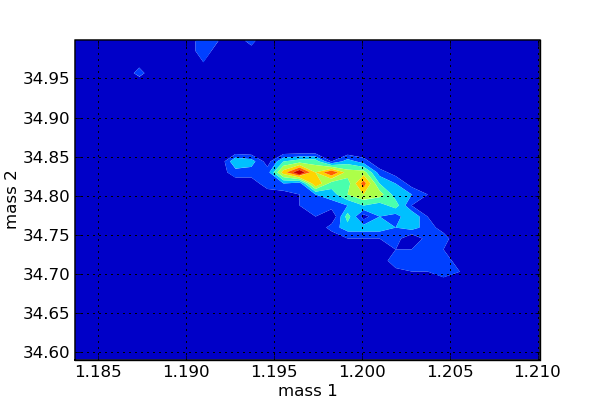
\includegraphics[scale=0.40]{m1m2_1905.png}
\caption{Parameter estimation for the recovered component masses $m_1$ and $m_2$ from the loud injection 1905}
\label{fig:figure24}
\end{minipage}
\hspace{0.5cm}
\begin{minipage}[b]{0.5\linewidth}
\centering
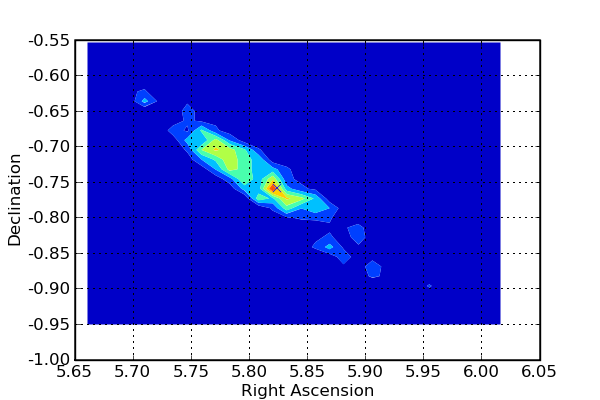
\includegraphics[scale=0.40]{RAdec_1905.png}
\caption{Parameter estimation for Right Ascension and declination from the loud injection 1905}
\label{fig:figure25}
\end{minipage}
\end{figure}

As seen from Figures ~\ref{fig:figure24} and ~\ref{fig:figure25} there are a series of improvements to the code that will be undertaken in the future: first a color scale for the probability in both $m_1m_2$ and $RAdec$ plots will be introduced so that the reader gets a better feeling of the results´ confidence; second sky localization in the simulation run can now be specified in GRB mode so that the code will look for a signal in a rather narrow sky window, not as in Figure ~\ref{fig:figure25} where the window is very large. As seen both in the tables above and in the plots the injection is found with a rather large Bayes factor and the parameter recovery looks to be more exact in the case of nested sampling analysis.
 
\paragraph{Quiet Injection}

The milestone for the Bayesian nested sampling code is the capability of finding and assigning signal status to a quiet simulation, that has an SNR comparable to the SNRs of loudest background triggers. After injecting several waveforms with different parameters, all having a recovered effective SNR of around 6-7, corresponding to background coincidences, the retrieved Bayes factors obtained vary in the region of Bayes factors from loud off-source events. This is, of course, unsatisfactory, hence a better investigation and/or a change in the code is necessary. It is obvious that by increasing the number of live points that the search is using, the sensitivity is increased, altogether with an increase in noise contribution. This, corroborated with running in --$GRB$ mode that limits the search on a narrow patch of sky around the specified GRB location may improve the capacity of finding such quiet signals.

I have tested the code on a quiet injection in --$GRB$ mode with an increase in the number of sampling points from 500 (the standard number used for the tests above) to 2000 and again, in the post-processing stage the number of live points was varied from 500 to 10000 in steps of multiplicity 2. For every increment of the number of sampling points there is an increment of the Bayes factor and a decrease in the precision with which the injected parameters are recovered. This is explained by the fact that the more data points are taken the more noise is analyzed as well. The table and plots below summarize the test results: Table 6 contains the injected parameters, Table 7 contains the recovered Bayes factors, chirp masses and inclinations and Figures 24 to 29 contain the $m_1-m_2$ and $RA-dec$ parameters for different numbers of live points in the post-processing mode.

\begin{table}[ht]
 \begin{tabular}{|l|l|l|l|l|l|l|l|l|l|}
 \hline
 \hline
 SNR & Waveform & Distance (Mpc) & $M_1$ & $M_2$ & $M_c$ & RA & dec & $\iota$ & Pol \\
 \hline
 \hline
 7.05 & GenPPN2PN & 19.75 & 1.43 & 2.52 & 1.64 & 5.71 & -0.68 & 1.60 & 0.95  \\
 \hline
 \hline
 \end{tabular} 
 \caption{Injected parameters for a quiet injection}
 \label{Table 6}
\end{table} 

\begin{table}[ht]
 \begin{tabular}{|l|l|l|l|l|}
 \hline
 \hline
 $N$ live & $logB_{SN}$ & $M_c$ & $D$ (Mpc) & $\iota$ \\
 \hline
 \hline
 500 & -12.94 & 2.63 & 74.04 & 1.57 \\
 \hline
 1000 & -6.13 & 2.61 & 75.85 & 1.57 \\
 \hline
 5000 & 7.21 & 3.32 & 84.15 & 1.62 \\
 \hline
 \hline
 \end{tabular} 
 \caption{Recovered $logB_{SN}$, $M_c$, distance $D$ and inclinations $\iota$ for $N=500$, $N=1000$ and $N=5000$ live points}
 \label{Table 7}
\end{table}   

\begin{figure}[ht]
\begin{minipage}[b]{0.5\linewidth}
\centering
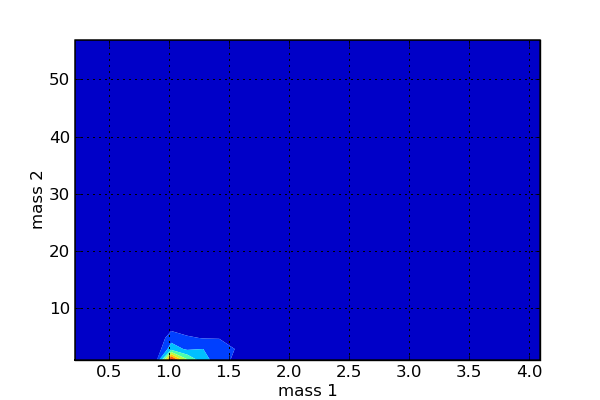
\includegraphics[scale=0.40]{m1m2_500.png}
\caption{Parameter estimation for the recovered component masses $m_1$ and $m_2$ for $N=500$ live points}
\label{fig:figure61}
\end{minipage}
\hspace{0.5cm}
\begin{minipage}[b]{0.5\linewidth}
\centering
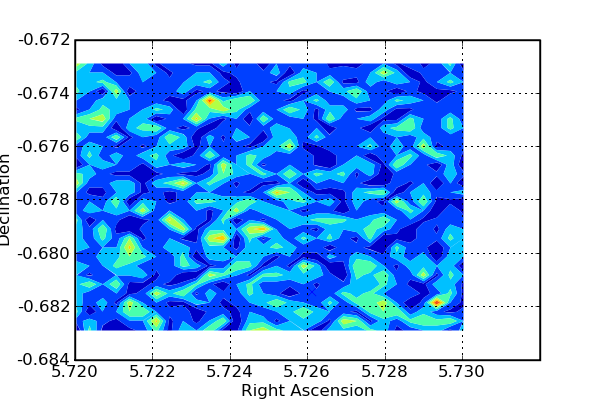
\includegraphics[scale=0.40]{RAdec_500.png}
\caption{Parameter estimation for Right Ascension and declination for $N=500$ live points}
\label{fig:figure62}
\end{minipage}
\end{figure}

\begin{figure}[h!]
\begin{minipage}[b]{0.5\linewidth}
\centering
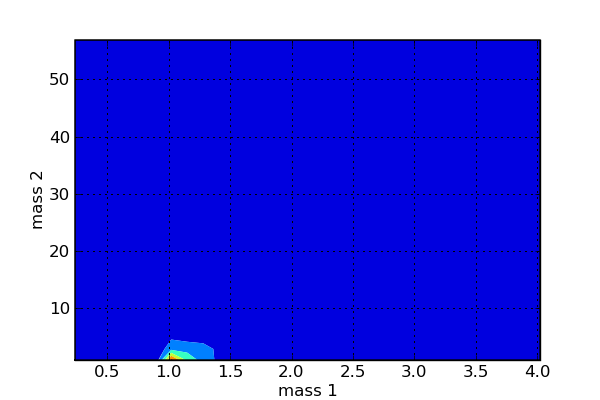
\includegraphics[scale=0.40]{m1m2_1000.png}
\caption{Parameter estimation for the recovered component masses $m_1$ and $m_2$ for $N=1000$ live points}
\label{fig:figure63}
\end{minipage}
\hspace{0.5cm}
\begin{minipage}[b]{0.5\linewidth}
\centering
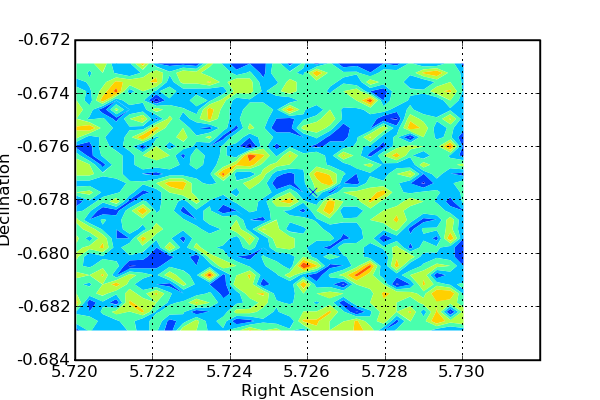
\includegraphics[scale=0.40]{RAdec_1000.png}
\caption{Parameter estimation for Right Ascension and declination for $N=1000$ live points}
\label{fig:figure64}
\end{minipage}
\end{figure}

\begin{figure}[h!]
\begin{minipage}[b]{0.5\linewidth}
\centering
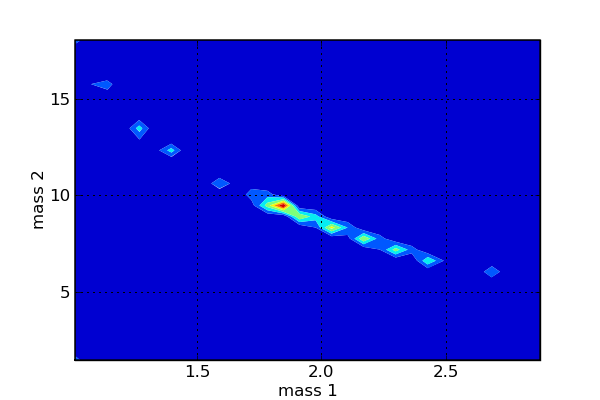
\includegraphics[scale=0.40]{m1m2_5000.png}
\caption{Parameter estimation for the recovered component masses $m_1$ and $m_2$ for $N=5000$ live points}
\label{fig:figure65}
\end{minipage}
\hspace{0.5cm}
\begin{minipage}[b]{0.5\linewidth}
\centering
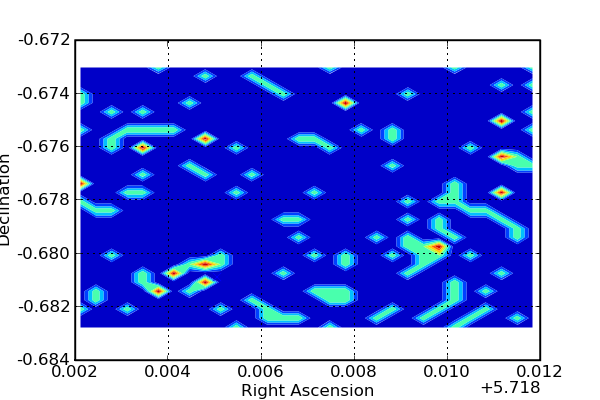
\includegraphics[scale=0.40]{RAdec_5000.png}
\caption{Parameter estimation for Right Ascension and declination for $N=5000$ live points}
\label{fig:figure67}
\end{minipage}
\end{figure}

The overall results obtained from analyzing this particular quiet injection are not satisfactory: the nested sampling code failed to find it as a potentioal GW signal, even though the recovered parameters fairly correspond to the ones injected. This might be caused by a possible undersampling of the low mass end and solutions are being proposed at the moment. As a next test, the initial mass limits on which the code works will be decreased, hence narrwoing the mass search window and hopefully decreasing the low mass undersampling.

\subsection{Future work}
Future work from my side will comprise of thoroughlly understanding the C code in which the nested sampling algorithm is written in, continuing the calibration tests for another quiet injection narrowing the masses search intervals this time and work on overall minimizing the computational costs of the algorithm. One idea raised by Dr. Stephen Fairhurst to decrease the analysis times would be to use the code as a follow-up in both GRB and radio transients searches and Taylor expand the prior distribution assuming that the inclination of the binary is a small angle. This would significantly simplify the integral in denominator in equation (39) and will hopefully make the analysis shorter.       


\begin{thebibliography}{99}

%inspiral
\bibitem{abbott2006} 
B. Abbott et al. (LIGO Scientific Collaboration): Phys. Rev. D {\bf 73}, 062001 (2006)

\bibitem{abbott2007}
B. Abbott {\it et al.} (LIGO Scientific Collaboration): \verb|//www.ligo.caltech.edu/docs/M/M060056-08/M060056-08.pdf|

%hulsetaylor
\bibitem{hulsetaylor} 
J. M. Weisberg, J. H. Taylor: in {\it Radio Pulsars}, ed by M. Bailes, D. J. Nice, S.  Thorsett (ASP. Conf.  Series, 2003)

%GRtheory
\bibitem{schutz} 
B. F. Schutz:{\it A First Course in General Relativity} (Cambridge University Press, 1985)

\bibitem{maggiore} 
M. Maggiore: {\it Gravitational Waves - Volume I - Theory and Experiments} (Oxford University Press, 2008)
\bibitem{leo}
L. P. Grishchuck {\it et. al}: Gravitational Wave Astronomy: in Anticipation of First Sources to be Detected, {\em astro-ph/0008481v3} (2001)

\bibitem{chaky}
I. Chakrabarty: Gravitational Waves: An Introduction, arXiv:physics/9908041v1 [physics.ed-ph] (1999)

\bibitem{cre}
W. Anderson and J. Creighton: Searches for Gravitational Waves from Binary Neutron Stars: A Review, arXiv:0712.2523v1 (2007)

%LIGOandGRB
\bibitem{ligoweb}
LIGO web page \verb| http://www.ligo.caltech.edu/|

\bibitem{LHOweb} 
LHO web page \verb| http://www.ligo-wa.caltech.edu/|

\bibitem{LLOweb} 
LLO web page \verb| http://www.ligo-la.caltech.edu/|

\bibitem{LIGOIFO} 
B. Abbott et al. (LIGO Scientific Collaboration): Nucl. Instrum.  Methods {\bf A517}, 154 (2004)

\bibitem{grb}
B. Abbott et al. (LIGO Scientific Collaboration): Search for Gravitational Waves associated with short GRBs in LIGO S5 data, paper draft

%chisquared
\bibitem{allen} B. Allen: {\em Phys. Rev. D} {\bf 71}, 062001 (2005).

%radioshit
\bibitem{lipunov}
Vladimir~M. Lipunov and Ivan~E. Panchenko, Pulsars revived by gravitational waves, {\em Astron. Astrophys.}, 312:937, 1996

\bibitem{hansen}
Brad M.~S. Hansen and Maxim Lyutikov, Radio and X-ray Signatures of Merging Neutron Stars, {\em Mon. Not. Roy. Astron. Soc.}, 322:695, 2001


\bibitem{moortgat1}
J.~Moortgat and J.~Kuijpers, Gravitational waves in magnetized relativistic plasmas, {\em Phys. Rev. D}, 70(2):023001, Jul 2004

\bibitem{moortgat2}
J.~{Moortgat} and J.~{Kuijpers}, Gravitational and magnetosonic waves in gamma-ray bursts, {\em Astronomy and Astrophysics}, 402:905--911, May 2003

\bibitem{usov}
Vladimir~V. Usov and Jonathan~I. Katz, Low Frequency Radio Pulses from Gamma-Ray Bursts?, 2000

\bibitem{nakar}
Ehud Nakar, Short-hard gamma-ray bursts, {\em Phys. Rep.}, 442:166--236, 2007

\bibitem{lorimer}
D.~R. Lorimer, M.~Bailes, M.~A. McLaughlin, D.~J. Narkevic, and F.~Crawford, A Bright Millisecond Radio Burst of Extragalactic Origin, {\em Science}, 318(5851):777--780, 2007

\bibitem{lofar1}
LOFAR webpage \verb|http://www.lofar.org/p/systems.htm|

\bibitem{lofar2}
A. G. de Bruyn {\it et al.} - LOFAR Science Case at \verb|http://www.lofar.org/PDF/NL-CASE-1.0.pdf|, (2002)

\bibitem{hyman}
Scott~D. Hyman {\it et al.} A powerful bursting radio source towards the Galactic Centre, {\em Nature.}, 434:50--52, 2005

\bibitem{zhu}
W. W. Zhu and Rex-Xin Xu GCRT J1745-3009: A freely precessing pulsar?, {\em Mon. Not. Roy. Astron. Soc. Lett.}, 365:L16, 2006

\bibitem{turolla}
R. Turolla, A. Possenti and A. Treves Is the bursting radio source gcrt j1745-3009 a double neutron star binary? {\em The Astrophysical Journal Letters}, 628(1):L49--L52, 2005

%nestedsampling
\bibitem{veitch}
J. Veitch and A. Vecchio: Assigning confidence to inspiral gravitational wave
candidates with Bayesian model selection, {\em Class. Quantum Grav.} {\bf 25} (2008) 184010 

\bibitem{skilling}
D. S. Sivia and J. Skilling: {\it Data Analysis, a Bayesian tutorial} (Oxford University Press, 2008)

\bibitem{ian}
J. W. Harry, First year report, Cardiff University, 2008

\bibitem{valeriu}
V. Predoi, BSc. Thesis, International University Bremen, 2006

\bibitem{wikiPSR}
Wikipedia on Hulse-Taylor pulsar: \verb| http://www.wikipedia.org|

\bibitem{craig}
C.A.K. Robinson, B.S. Sathyaprakash, Anand S. Sengupta: A geometric algorithm for efficient coincident detection of gravitational waves, 	arXiv:0804.4816v1 [gr-qc] (2008)

\bibitem{radioprop}
J. Clark {\it et al.} Proposal to the LSC and Virgo: Joint observations with radio telescopes, submitted to the LSC-Virgo, September 2009 

\end{thebibliography}




\end{document}
